\documentclass[
%draft,           %use this for fast draft compilation with additional overfull boxes hint bars (also affects graphicx)
a4paper,          %A4 paper size
11pt,             %well readable for A4 printing
cleardoubleempty, %nice left plain pages before chapters
%chapterprefix,    %chapter X prefix before chapters
%appendixprefix,   %appendix X prefix before appendices
headsepline,      %lines in header
headtopline,      %lines in header
footbotline,      %lines in footer
footsepline,      %lines in footer
plainfootbotline, %lines in footer for scrplain page style
plainfootsepline, %lines in footer for srcplain page style
ilines,
DIV18,            %adjust this value for more/less text on pages
BCOR5mm]{scrbook}
\usepackage[]{scrpage2} %%% koma script for nice layout
\usepackage[english, ngerman]{babel}   %%% an english thesis usually has a german synopsis

% \usepackage{scrltx}
%\usepackage{layout}  %%% may be needed if i steal some more code from other thesises
\usepackage{exscale} %%% for proportional sum and integral signs

\usepackage[
    backend=bibtex, 
    natbib=true, 
    sorting=none,
    %bibstyle=verbose, 
    %citestyle=verbose,    % bibstyle extensively modifed below
    doi=true, url=true,                     % excluded from citations below
    citecounter=true, citetracker=true,
    block=space, 
    backref=true, backrefstyle=none,
    abbreviate=false,
    isbn=true
]{biblatex}
\addbibresource{Misc/bibliography.bib}

%\usepackage{struktex} %%% create structograms
\usepackage{booktabs} %%% scientific publication style tables
\usepackage{empheq}   %%% for boxed equations and alike
\usepackage{xcolor,colortbl}  %%% for colored text, formulae and tables
\usepackage{amsmath}  %%% math symbols needed
\usepackage{amsfonts} %%% math fonts needed
\usepackage{amssymb}  %%% maths symbols needed 
\usepackage{amsthm}   %%% theorem environments
\usepackage{dsfont}   %%% for blackboard numbers and characters 
%\usepackage{mathdots/mathdots}

\usepackage{fancybox} %%% more types of boxes 

\usepackage{graphicx}       %%% CUSTOMIZATION: include all pictures
%\usepackage[draft]{graphicx} %%% choose draft option for faster compiling without pictures
\graphicspath{{Figures/}}      %%% all pictures will reside there and in subdirs

%\usepackage[rlft]{floatflt} %%% allows text wraping of floating figures 
\usepackage{float}      %%% define custom float environments
\usepackage[plainpages=false]{hyperref} %%% CUSTOMIZATION use this package for the final compilation run for online publication, includes hyperlinks for sections/eqs/etc.
%\usepackage[]{hyperref} %%% CUSTOMIZATION use this package for the final compilation run for online publication, includes hyperlinks for sections/eqs/etc.
%\usepackage{subfigure}  %%% nice captioning and referencing of subfigures
\usepackage{subcaption}
\usepackage{caption}    %%% (load after subfigure package) nicer layout for figure captions
%\usepackage[notref,notcite]{showkeys} %%% show labels for equations and pictures on the margin(intended for development state) 


%%%%%%%%%%%%%%%%%%%%%%%%%%%%%%%%%%%%%%%%%%%%%%%%%%
%%% Selection of the fonts!!
\usepackage[T1]{fontenc}
\usepackage{helvet}
%%%%%%%%%%%%%%%%%%%%%%%%%%%%%%%%%%%%%%%%%%%%%%%%%%

%ANNES PACKAGES
\usepackage{siunitx}
\usepackage[above]{placeins}
\usepackage{stfloats}
\usepackage[utf8]{inputenc}
\usepackage[T1]{fontenc}
\usepackage[italic]{hepnames}
\usepackage[final]{pdfpages} %set to "final" in the end to show the pdf page
\usepackage{multirow}
\usepackage{multicol}
\usepackage{verbatim}
\usepackage{rotating}
\usepackage{array} 
\usepackage{pifont}
\usepackage{setspace}
\usepackage{textcomp}
\usepackage{siunitx}
\usepackage{bm}
\usepackage{upgreek}
%\usepackage[]{units}
\usepackage{tabularx}
\usepackage[super]{nth} %e.g. for 20th century -> \nth{20} century
\setcounter{tocdepth}{3}
\setcounter{secnumdepth}{3}

\usepackage{wrapfig}%for wrapping text around figures

\usepackage{todonotes} %Added by Phill so that todo lists can be added
\setlength{\marginparwidth}{2cm} %This stops the todo notes from overflowing the page

\setlength{\parskip}{\baselineskip}%
\setlength{\parindent}{0pt}%

\newcommand{\myparagraph}[1]{\thesubsubsection\ \alph{paragraph}{#1}\mbox{}\newline}
\newcommand{\redcomment}[1]{\ding{110}\ding{43}\textcolor{red}{#1}}

\newcommand{\slic}{\textsc{SLIC}\xspace}
\newcommand{\gdml}{\textsc{GDML}\xspace}
\newcommand{\xml}{\textsc{XML}\xspace}
\newcommand{\lcdd}{\textsc{LCDD}\xspace}
\newcommand{\lcio}{\textsc{LCIO}\xspace}
\newcommand{\ilcsoft}{\textsc{ILCSoft}\xspace}
\newcommand{\marlin}{\textsc{Marlin}\xspace}
\newcommand{\Root}{\textsc{ROOT}\xspace}
\newcommand{\Cplusplus}{\texttt{C++}\xspace}
\newcommand{\geant}{\textsc{Geant4}\xspace}
\newcommand{\bdsim}{\textsc{BDSIM}\xspace}
\newcommand{\mucarlo}{\textsc{MUCARLO}\xspace}
\newcommand{\turtle}{\textsc{TURTLE}\xspace}
\newcommand{\fluka}{\textsc{FLUKA}\xspace}
\newcommand{\flair}{\textit{flair}\xspace}
\newcommand{\degree}{\ensuremath{^\circ}}
\newcommand{\electron}{e$^-$\xspace}
\newcommand{\positron}{e$^+$\xspace}
\newcommand{\lumi}{$\mathcal{L}$\xspace}

\DeclareSIUnit\gauss{G}

%------Definition for column color in table
\definecolor{Gray}{gray}{0.9}
\newcolumntype{g}{>{\columncolor{Gray}}r}
%-----------------------------------------

%SIMONS COMMANDS FOR TITLEPAGE
\usepackage{tikz}
\def\changemargin#1#2{\list{}{\rightmargin#2\leftmargin#1}\item[]}
\let\endchangemargin=\endlist 
\usepackage[absolute]{textpos}
\newcommand{\changefont}[3]{
\fontfamily{#1}\fontseries{#2}\fontshape{#3}\selectfont}

\newcommand{\myname}{Anne Schütz}
\newcommand{\mytitle}{Optimizing the design of the Final-Focus Region\\for the International Linear Collider}
\newcommand{\myinstitute}{Institute of Experimental Nuclear Physics (IEKP)}
\newcommand{\mydepartment}{Department of Physics}
\newcommand{\myuniversity}{Karlsruhe Institute of Technology}

\newcommand{\reviewerone}{Prof. Dr. Günter Quast (IEKP)}
\newcommand{\reviewertwo}{Prof. Dr. Eckhard Elsen (DESY)}
\newcommand{\advisor}{Dr. Marcel Stanitzki (DESY)}


\newcommand{\timestart}{April 01, 2015}
\newcommand{\timeend}{March 31, 2018}
%\newcommand{\submissiontime}{DD. MM. 20XX}

%%%%%%%%%%%%%%%%%%%%%%%%%%%%%%%%%%%%%%%%%%%%%%%%%%
%%% user defined abbreviations/commands/macros/layout commands

\input{Macros/layout.tex}

%%%%%%%%%%%%%%%%%%%%%%%%%%%%%%%%%%%%%%%%%%%%%%%%%%




%%%%%%%%%%%%%%%%%%%%%%%%%%%%%%%%%%%%%%%%%%%%%%%%%%
%%% the document starts here
\begin{document}
\frontmatter       %%% use different numbering format for pages
\pagestyle{empty}  %%% for special pages, chose a simple layout

\selectlanguage{english}
%\include{Misc/KIT_titlepage} %%% force a right side page with \include
%\cleardoublepage

\pagestyle{scrheadings}    %%% for normal text, display section names in header line
\selectlanguage{ngerman}
%\chapter*{Zusammenfassung}
\addcontentsline{toc}{chapter}{Zusammenfassung} 
Der ``International Linear Collider'' (ILC) ist ein geplanter Linearbeschleuniger f\"ur die Kollisionen von Elektronen und Positronen bei einer anf\"anglichen Schwerpunktsenergie von \SI{250}{\GeV}.
Mit seinen Forschungszielen steht er in einem erg\"anzenden Zusammenhang mit dem ``Large Hadron Collider'' (LHC).
Denn nach der Entdeckung des Higgs-Bosons am LHC in 2012 ist eines der Ziele des ILC, die Eigenschaften und Wechselwirkungen des Higgs-Bosons und des Top-Quarks mit nie dagewesener Präzision zu messen.
Auch die Suche nach Teilchen aus Modellen jenseits des Standardmodells, welche ebenfalls auf dem Programm der verschiedenen ILC-Phasen steht, wird durch diese Präzision erleichtert.

Sowohl das Layout des Beschleunigers als auch das der Detektoren muss optimiert werden, um Untergrundraten unterhalb einer gewissen Grenze zu halten und damit die angestrebte Pr\"azision zu erreichen.
Hierzu wurden einige Studien durchgeführt, um unterschiedliche Untergrundquellen zu untersuchen und die Raten im \sid Detektor, einer der beiden f\"ur den ILC vorgeschlagenen Detektorexperimente, zu analysieren.
Diese Studien basieren auf Monte Carlo Generatoren, welche Untergrundereignisse aus verschiedenen Quellen simulieren.
Nach einer vollen Detektorsimulation wurden diese Ereignisse dann in Hinsicht auf die \sid Detektorokkupanz beurteilt.
Liegt diese Okkupanz nahe oder sogar oberhalb der von der \sid-Gruppe festgelegten Akzeptanzgrenze, so wurden Vorschläge zur Beschleuniger- und Detektoroptimierung unterbreitet und getestet, mit denen die Okkupanz reduziert werden kann.

Zu den hier untersuchten Untergründen gehören sowohl der \positron\electron-Paaruntergrund, der durch die Wechselwirkung der elektromagnetischen Felder der kollidierenden Strahlb\"undel entsteht, als auch der Myonen-Maschinenunter-grund aus der Wechselwirkung des Strahls mit den Beschleunigerinstrumenten, sowie der Neutronenuntergrund, der von den Strahl-Dumps aus in Richtung der Detektoren gerichtet ist.
Die Abhängigkeit des \positron\electron-Paaruntergrundes von den ILC-Strahlparametern wurde f\"ur die in 2017 beantragte Änderung der Parameter f\"ur die erste ILC-Phase evaluiert.
Die Ergebnisse der in der vorliegenden Arbeit präsentierten Studie haben dabei zur Entscheidungsfindung maßgeblich beigetragen.
\\Zusätzliche Studien umfassen die Untersuchung des Designs der Strahl-Dumps im Hinblick auf die Bestrahlungsdosis in der Dump-Halle.
Neben den Simulationsstudien wurden auch Messungen in der japanischen Beschleunigeranlage ``Accelerator Test Facility 2'' durchgeführt, um die Maschinenuntergrundrate in Abhängigkeit von verschiedenen Beschleunigerzust\"anden zu messen.
Das Ziel war hierbei die Funktionalität eines Strahlkollimators zu testen.

Bei allen präsentierten Studien werden Vorschläge zur Beschleuniger- und Detektoroptimierung genannt, um die Untergrundraten in \sid zu reduzieren und somit die geplanten Pr\"azisionsmessungen ermöglichen.
\selectlanguage{english}
%\chapter*{Abstract}
\addcontentsline{toc}{chapter}{Abstract} 
The International Linear Collider (ILC) is a proposed linear electron positron collider with a center-of-mass energy of \SI{250}{\GeV} in its first stage.
After the discovery of the Higgs boson at the Large Hadron Collider (LHC) at CERN in 2012, the physics goals of the ILC include the measurements of the Higgs boson properties and its interactions, but also measurements of the top quark and searches beyond the Standard Model are part of the ILC program in the different ILC stages.
The ILC, however, is in competition with the LHC, but is a complementary collider experiment, since it is aimed at unprecedented precisions rather than at high collision energies.
\\In order to achieve such precisions, both the accelerator design and the detector designs have to be optimized with respect to limiting the detector background below an acceptable limit.
For the evaluation of various background sources, different Monte Carlo event generators have been used to generate background events that were then analyzed in a full detector simulation of the \sid detector.
\sid is one of the proposed detector concepts for the ILC, for which a specific critical acceptance limit for background rates has been set.
Throughout the chapters of this thesis, the acceptance limit has been used to assess the arising background occupancy in \sid.
If the occupancy has been found to be close to or to exceed the limit, possibilities to reduce the background level have been tested and recommendations for design optimizations have been made.
\\The presented background simulation studies contain three major background sources: the \positron\electron pair background from beam-beam interactions, the machine background created by interactions of the beam with the accelerator components, and the neutron background produced in the ILC main beam dumps.
The pair background was studied with respect to its dependency on different ILC running schemes, such as the proposed changes in the beam parameter sets for the ILC stage at \SI{250}{\GeV}.
The results of these studies have been used in 2017 to inform the ILC design decision regarding these beam parameters.
\\In addition to the background study for the main beam dumps, the beam dump designs that are based on water dumps have also been analyzed with respect to the arising irradiation of the surroundings.
Besides the mentioned simulation studies, measurements of the machine background in dependency of certain accelerator conditions have been performed at the Accelerator Test Facility 2 at KEK in Japan.
The goal of these measurements was to validate the functionality of a recently installed vertical beam halo collimator that is planned to be used at the ILC as well.
\\For all the presented topics, recommendations for accelerator and detector design optimizations are given, with which the background level in the \sid detector can be reduced in order to facilitate the aimed-for precision at the ILC.

%%% use english language from this point
\selectlanguage{english}
\tableofcontents         %%% create a TOC
\listoffigures
\listoftodos

\mainmatter              %%% now the thesis really starts
\chapter{Introduction}
\label{Introduction}
Since the 1920's, accelerator physics research has been rapidly advancing, and with it, so is high-energy particle physics.
Starting with the first accelerating structures, which could accelerate particles to no more than a few hundred \si{\keV}, the reach to higher and higher center-of-mass energies requires new inventions in the field of particle accelerators.
Along with this goes the development of particle detectors, which need to adapt to the increasingly demanding environments of particle collisions that are created by the high-performing colliders.
Also other areas benefit from the fast pace in the research efforts and scientific breakthroughs, such as the development of sensor technologies for mobile phones, materials for the aerospace industry, or medical applications like cancer therapy.
High-energy and accelerator physics are therefore pioneering in many different scopes.

In the field of particle physics, discoveries of new particles and measurements of their characteristics have given explanations and insights to some of the key questions about the composition of matter, the fundamental forces that describe all physical interactions, and about the beginning of the universe.
The first experimental evidence of the Higgs boson in 2012~\cite{Higgs,Higgs2} was the discovery of one of the missing pieces in the current understanding of the fundamental building blocks of the universe.
This was accomplished at the Large Hadron Collider (LHC) at CERN~\cite{LHC_CERN}.
With the LHC being the particle collider with the world's highest nominal collision energy of \SI{14}{\TeV}, the pursuit for the highest energies has reached its peak for the moment.
This does however not mean that the end of this pursuit is near, future colliders at the energy frontier are proposed for the coming decades.

After a synopsis of the current knowledge of fundamental particle physics and accelerator physics in Chapters~\ref{Lepton_Physics} and~\ref{LinearColliderPhysics}, it will be derived that colliders at the energy frontier need a complementary collaborator in order to provide a complete understanding of open issues of particle physics, such as the properties of the Higgs boson.
The International Linear Collider (ILC) is such a collaborator.
It is a proposed linear electron positron collider designed for high-energy physics experiments, not at the energy frontier but at the precision frontier.
Its collision energy will hence be in the range of \SI{250}{\GeV} to \SI{1}{\TeV}, aiming to measure particle physics processes with unprecedented precision.
Chapter~\ref{ILC} will give an overview of the ILC accelerator design and its detector experiments, and will motivate its physics goals.
An important goal is the measurements of the Higgs boson couplings to elementary particles.
Due to the high precision, the ILC will be able to measure these couplings to $\sim$\,\SI{1}{\percent} accuracy, which is needed to distinguish different physics models.
Herein lies the discovery potential of the ILC.

In order to achieve these goals, precision detector experiments are needed with high tracking resolutions and granular calorimeter designs.
To this end, the detector requirements are strict, and emphasize a low material budget for improving the tracking performance.
The ILC aims for nanometer-sized beams to gain high luminosities and to allow the experiments' vertex detector to have a minimal radius.
This leads to high vertex reconstruction efficiencies, but also to the fact that the detector environment has to rely on minimal background levels.
If the occupancy in the innermost subdetectors is too high, the vertex detector performance declines and the ILC goal of unprecedented precision cannot be achieved.

A complete understanding of the detector background and its impact on the detector performance is therefore crucial, especially because of the ILC beam timing structure and the readout architecture of the detectors.
Chapters~\ref{PairBkg} -~\ref{BeamDumps} present detailed studies of various background sources, and show that the background can be constrained by optimizing the accelerator and the \sid detector layout.
\sid is one of the two proposed detector experiments for the ILC, and the focus of the presented detector occupancy studies.
The chapters are sorted by beam induced backgrounds, machine backgrounds, and backgrounds from the ILC main beam dumps.
All of these backgrounds originate inside the detectors (in the case of the beam induced backgrounds), or in parts of the ILC accelerator close to the detectors.
The results of the studies have been used to inform design decisions of the ILC accelerator on different topics.

First, the simulation studies concerning the substantial \positron\electron pair background arising from beam-beam interactions will be discussed in Chapter~\ref{PairBkg}.
Since this background is directly dependent on ILC running schemes, various studies of its dependencies have been conducted.
A study of the timing of the background hits in the individual \sid subdetectors gave hints on how to reduce the background occupancy further.
\\Chapters~\ref{BDS_Muons} and~\ref{machine_bkg} then investigate the backgrounds from the interaction of the beam with machine components, and the possibilities to reduce these backgrounds.
Chapter~\ref{BDS_Muons} presents a simulation study of the muon background from the ILC Beam Delivery System, whereas for Chapter~\ref{machine_bkg} both direct measurements and simulation studies of machine background levels at the Accelerator Test Facility 2 were done.
\\Finally, as discussed in Chapter~\ref{BeamDumps}, the ILC main beam dumps present another source of detector background, and have been studied in a detailed simulation.
Due to their current design, several issues have to be addressed, not only because of the arising background but also because of the irradiation of the beam dump surroundings.

The results of all studies done for this thesis are then summarized in Chapter~\ref{Results}.
It shows that analyzing the sources of background in detail provides crucial input for the optimization of the ILC accelerator itself.
Recommendations are given for optimizing the accelerator with respect to the beam parameters and possible shielding options for the Final-Focus region, which contains the parts of the ILC close to the detectors.
Afterwards, the detector collaborations have to consider the impact of the background in the design of the detector geometry and its readout architecture, and refine them accordingly.
Also here, recommendations for the \sid detector have been made.
This will bring the ILC closer to its goal of measurements at unprecedented precision.          %%% include all chapters in order
\chapter{Physics at lepton colliders}
\label{Lepton_Physics}
\begin{chapterabstract}
The physics at particle colliders, where two particle beams are brought into collision, is the physics of atoms and quanta, of nuclei and partons, of particles that build up everything we know, but also of new particles, physics beyond our current knowledge.
After a brief introduction of the Standard Model (a theory describing the elementary particles and the fundamental forces) in Section~\ref{StandardModel}, the physics processes including their production modes (Section~\ref{Production_modes}) and background processes (Section~\ref{Backgrounds}) at a lepton collider will be explained in more detail.
\end{chapterabstract}
\vspace*{0.5cm}\newline 
\noindent
Particle physics extends back to the ancient Greek times, when the idea was developed that matter is made of ``indivisible'' (\'atomos, Greek) parts.
Atoms are, in fact, not indivisible at all.
When the electron was experimentally discovered in 1897 by J.J. Thomson, it was proposed that these particles must be a component of every atom~\cite[p. 13ff]{Griffiths}.
This sparked the interest of many physicists in the early \nth{20} century to perform experiments probing atoms.
One of them was Ernest Rutherford, who fired alpha particles\footnote{Alpha particles are the nuclei of Helium atoms. Ernest Rutherford obtained them from decays of uranium and other radioactive elements.} through a thin gold foil, and thereby found that atoms are mostly empty with a positively charged nucleus that is only a fraction of the size of the atom itself~\cite{GoldFoil}.
This discovery was a crucial step towards the modern atomic model.

Closer to our current understanding of the atomic model is the Bohr model, developed by Niels Bohr in 1914~\cite[p. 15]{Griffiths}.
It asserts that electrons orbit the positively charged nucleus on stable shells with distinct radii.
The shells correspond to discrete energies, such that an electron switching from one shell to a shell with a larger or smaller radius would have to absorb energy, or emit energy respectively.
This energy quantum is absorbed or emitted in the form of light, or more precisely, in the form of a photon.
Nowadays, it is known that the electrons do not orbit the nucleus on discrete shells but rather in orbital zones, where the electron has a higher probability to be observed.

In order for an atom to have a neutral charge, the number of electrons in the atomic shells has to be balanced by an equal amount of positive charge in the nucleus.
It was already proven by Rutherford that nuclei of different atoms are built from the hydrogen nucleus.
He thereby discovered the proton, and explained that the positive charge of the nucleus is the summed up charges of the protons inside the nucleus.
In 1932, it was found that atoms can not only consist of electrons and protons.~\cite[p. 15]{Griffiths}
The mass measurements of various isotopes showed that their masses differed by concrete amounts.
The explanation was that the nucleus must consists of protons and particles with a similar mass but a neutral charge, the neutrons.
Isotopes are therefore atoms of the same element with the same number of electrons and protons, but with a different amount of neutrons.

Over the years, the development of particle accelerators that can accelerate particles to higher and higher energies allowed to probe even the constituents of the atom.
This showed that the end had not been reached yet, that protons and neutrons are not elementary but composite particles.
Their partons, the quarks and gluons, are part of the current theory of all elementary particles and the fundamental forces they interact with, the Standard Model.

\section{The Standard Model}
\label{StandardModel}
The Standard Model (SM) was developed and formulated around the 1960s and 1970s, when the theories of the electromagnetic and the strong interaction, namely quantum electrodynamics (QED)~\cite{QED,QED2,QED3} and quantum chromodynamics (QCD)~\cite{QCD,QCD2}, were combined into one mathematical model that explains how the elementary particles interact with each other via the fundamental forces of the universe~\cite[p. 3]{Griffiths}.
Since then, high-energy particle physics experiments could verify the SM predictions so well, that it has proven itself to currently be the best theoretical model of all subatomic particles that we know of.
The most recent measurements of the masses and other SM properties of the particles are summarized by the Particle Data Group (PDG) in the ``Review of Particle Physics'' in yearly editions~\cite{PDG}.

The SM differentiates between two classes of fundamental particles: 
the particles that make up all matter are called \textit{fermions}, whilst the force mediators, through which the fermions can interact, are called \textit{gauge bosons}.
\begin{figure}[htbp]
\centering
\includegraphics[width=0.55\textwidth]{Figures/Standard_Model_of_Elementary_Particles.png}
\caption[Table of the elementary particles of the Standard Model]{The Standard Model describes all elementary particles, the twelve fermions in their three generations and the four gauge bosons, as well as the Higgs boson.
The shadows indicate possible interactions between the fermions and gauge bosons~\cite{SM}.}
\label{fig:SM}
\end{figure}

\paragraph{Fermions}
Fermions are particles with a half-integer spin $s$ as one of their quantum numbers. 
The spin has a direction, and a specific amplitude, which can be calculated as $\frac{h}{2\pi}\sqrt{s(s+1)}$, with $h$ being the Planck constant~\cite[p. 121]{Griffiths}.
All fermions have a specific set of quantum numbers, so that by giving the electric charge, the spin, and the flavor, all fermions can be identified precisely.
Table~\ref{tab:Fermions} lists all Standard Model fermions with their quantum numbers.
\begin{table}
\caption[Quantum numbers of the Standard Model fermions]{Quantum numbers of the Standard Model fermions. 
The table lists the values for the electric charge $q$, and the spin $s$ for all fermions, as well as the lepton number $L$ of the leptons and the quark flavor of the quarks. 
Their respective antiparticles are highlighted by the shaded background~\cite[cf. p. 49]{Griffiths}.}
\label{tab:Fermions}
\centering
\begin{tabularx}{\textwidth}{c|c|rrrrr|@{\hskip 0.03in}|c|rrrrrrrr}
\hline\hline
& Leptons & $q$ & $s$ & $L_e$ & $L_{\mu}$ & $L_{\tau}$ & Quarks & $q$ & $s$ & $U$ & $D$ & $C$ & $S$ & $T$ & $B$\\
\hline
& e\textsuperscript{\textendash} & -\,1 & 1/2 & +1 & 0 & 0 & u & +2/3 & 1/2 & +1 & 0 & 0 & 0 & 0 & 0\\
\rowcolor{Gray}
\cellcolor{white}& e\textsuperscript{+} & +1 & 1/2 & -\,1 & 0 & 0 & $\bar{\rm{u}}$ & \textendash2/3 & 1/2 & -\,1 & 0 & 0 & 0 & 0 & 0\\
& $\upnu$\textsubscript{e} & 0 & 1/2 & +1 & 0 & 0 & d & -\,1/3 & 1/2 & 0 & -\,1 & 0 & 0 & 0 & 0\\
\rowcolor{Gray}
\multirow{-4}{*}{\rotatebox[origin=c]{90}{\parbox[c]{1.9cm}{\cellcolor{white}\centering First generation}}} &$\bar\upnu$\textsubscript{e} & 0 & 1/2 & -\,1 & 0 & 0 & $\bar{\rm{d}}$ & +1/3 & 1/2 & 0 & +1 & 0 & 0 & 0 & 0\\
\hline
& $\upmu$\textsuperscript{\textendash} & -\,1 & 1/2 & 0 & +1 & 0 & c & +2/3 & 1/2 & 0 & 0 & +1 & 0 & 0 & 0\\
\rowcolor{Gray}
\cellcolor{white}&$\upmu$\textsuperscript{+} & +1 & 1/2 & 0 & -\,1 & 0 & $\bar{\rm{c}}$ & \textendash2/3 & 1/2 & 0 & 0 & -\,1 & 0 & 0 & 0\\
& $\upnu$\textsubscript{$\upmu$} & 0 & 1/2 & 0 & +1 & 0 & s & -\,1/3 & 1/2 & 0 & 0 & 0 & -\,1 & 0 & 0\\
\rowcolor{Gray}
\multirow{-4}{*}{\rotatebox[origin=c]{90}{\parbox[c]{1.9cm}{\cellcolor{white}\centering Second generation}}}& $\bar\upnu$\textsubscript{$\upmu$} & 0 & 1/2 & 0 & -\,1 & 0  & $\bar{\rm{s}}$ & +1/3 & 1/2 & 0 & 0 & 0 & +1 & 0 & 0\\
\hline
& $\uptau$\textsuperscript{\textendash} & -\,1 & 1/2 & 0 & 0 & +1 & t & +2/3 & 1/2 & 0 & 0 & 0 & 0 & +1 & 0\\
\rowcolor{Gray}
\cellcolor{white}& $\uptau$\textsuperscript{+} & +1 & 1/2 & 0 & 0 & -\,1 & $\bar{\rm{t}}$ & \textendash2/3 & 1/2 & 0 & 0 & 0 & 0 & -\,1 & 0\\
& $\upnu$\textsubscript{$\uptau$} & 0 & 1/2 & 0 & 0 & +1 & b & -\,1/3 & 1/2 & 0 & 0 & 0 & 0 & 0 & -\,1\\
\rowcolor{Gray}
\multirow{-4}{*}{\rotatebox[origin=c]{90}{\parbox[c]{1.9cm}{\cellcolor{white}\centering Third generation}}}& $\bar\upnu$\textsubscript{$\uptau$} & 0 & 1/2 & 0 & 0 & -\,1 & $\bar{\rm{b}}$ & +1/3 & 1/2 & 0 & 0 & 0 & 0 & 0 & +1\\
\hline\hline
\end{tabularx}
\end{table}
\\Fermions are further categorized as \textit{leptons} and \textit{quarks}, as well as in three generations, which can be seen in Figure~\ref{fig:SM}.
Among the leptons are the electron and its heavier brothers, the muon and the tau.
In their respective generation, each of them has a neutrino, respectively named the electron-neutrino, muon-neutrino, and tau-neutrino.
They are electrically neutral particles.

Additionally, every particle has an antiparticle, so there are actually not only six leptons but twelve.
The SM does in general not remark the antiparticles, because it assumes that the physics of particles and antiparticles is the same.
The only difference between them is the sign of their internal quantum numbers:
The electron's antiparticle is the positron, which has the same mass and spin as the electron, but has a positive electric charge of +1, and a negative lepton number $L_e$ of -\,1.
The antiparticles of the muon ($\upmu$\textsuperscript{-}) and the tau ($\uptau$\textsuperscript{-}) hence are $\upmu$\textsuperscript{+} and $\uptau$\textsuperscript{+}, respectively.
As neutrinos on the other hand have no electric charge, they can only be distinguished from their respective antineutrino by their lepton number and their helicity.
The helicity describes the state of the particle's spin direction in comparison to the particle's momentum.
When the spin direction and the momentum are parallel, the particle is called right-handed.
It is called left-handed, when they are antiparallel.
In the SM, neutrinos are always left-handed, whilst antineutrinos are right-handed. %Weak force, parity violation

Every generation of quarks consists of one up- and one down-type quark, where the up-type quarks have an electric charge of 2/3, whilst down-type quarks have a charge of -\,1/3.
However, they do not only carry the electric charge, but also the so-called color charge.
The color charge is unrelated to the common meaning of color.
The different quark colors are used as quantum numbers to differentiate between quarks.
Every quark has one of three colors (red, green, and blue), every antiquark has one of three anti-colors (anti-red, anti-green, and anti-blue).
Thus, there are overall 36 different quarks and antiquarks.
Due to the law of confinement, there can only be color-neutral particles.
Quarks are therefore not free, but hadronize and form a bound state together with other quarks.
These bound quark states, called hadrons, consist of several quarks.
A particle with a quark of a specific color and an antiquark of the corresponding anti-color is called a meson.
Together, the color and anti-color of the quarks make the meson color-neutral.
A baryon, which is a particle with three quarks, can only be color-neutral when it carries three quarks with three different colors (or anti-colors), so red\textendash green\textendash blue or anti-red\textendash anti-green\textendash anti-blue, any other combination is not possible.
%Finally, the penta-quarks are bound states of five quarks, where three of them form a color triplet like a baryon, and the remaining two form a color-anticolor pair like a meson.

In everyday nature, the only observable hadrons are the protons and neutrons due to their constituents.
They are baryons, hence are built from three quarks:
protons contain two up-quarks and one down-quark, giving the proton its positive electric charge of +1.
Neutrons on the other hand are formed by one up-quark and two down-quarks, resulting in an electrically neutral particle. 
As the up-quark is the lightest quark, it is stable and does not decay.
All other quarks decay after certain lifetimes into another quark with smaller mass.
That is the reason why all hadrons that are produced artificially in a high-energy particle collider are unstable.
Since the down-quark is the second lightest quark, it can decay into the up-quark, giving reason to the spontaneous decay of free neutrons into protons when one of the down-quark decays.
The proton is the lightest existing baryon, and can not decay further according to the Standard Model, since its quantum numbers have to be conserved.
Together, the protons and neutrons construct the nuclei of every atom of every element.
%The masses of the quarks increases towards higher generations.
\begin{table}[htbp]
\caption[Fundamental forces: effective strength and mediators]{The fundamental forces and their mediators~\cite[cf. p. 59]{Griffiths}.
The strength of a force is dependent on various external factors, such as its source and its distance to the observer.
Therefore, the listed values are a rough guideline of the orders of magnitude of difference between the effective strengths of the forces.}
\label{tab:Forces}
\centering
\begin{tabularx}{0.45\textwidth}{l|ll}
\hline\hline
Force & Strength & Mediators\\
\hline
Strong & \num{10} & Gluons\\
Electromagnetic & \num{e-2} & Photons\\
Weak & \num{e-13} & W, Z\\
Gravitational & \num{e-42} & Gravitons\\
\hline\hline
\end{tabularx}
\end{table}

\paragraph{Bosons}
The \textit{gauge bosons} described in the SM are the force mediators of the fundamental forces of nature:
the electromagnetic, the weak, and the strong force.
Gravity is the only fundamental force that is not represented by the SM.
On the scale of ranges in particle physics, it is by far the weakest force, as can be seen from Table~\ref{tab:Forces}.
\\The fermions explained in the paragraph above are subject to these fundamental forces, and can interact with each other by exchanging the force mediators.
The mediating particles are gauge bosons, which are particles with an integer spin.\\
\begin{minipage}{0.55\textwidth}
The \textit{photon} is a massless, electrically neutral particle mediating the electromagnetic (EM) force between electrically charged particles only.
The photon couples therefore to all charged SM particles and their antiparticles, such that the electric charge is conserved in this interaction.
The EM interaction, which is pictured in a Feynman diagram in Figure~\ref{fig:Feynman:EM}, does not change the flavor of the particle.
%The mathematically formulated theory of all interactions involving the electromagnetic force in the context of particle physics is given in the theory of quantum electrodynamics (QED).
%Although its reach is in principle not limited by its mass, the effective range of the electromagnetic force is dependent on its potential, which scales with $1/r$. \todo{Potential of electroweak interaction}
\end{minipage} \hfill
\begin{minipage}{0.4\textwidth}
\centering
\begin{figure}[H]\centering
\includegraphics[width=0.5\textwidth]{Feynman_diagrams/Jaxo_EM.png}
\caption{SM Feynman diagram of the EM interaction}
\label{fig:Feynman:EM} 
\end{figure}
\end{minipage}

\noindent\begin{minipage}{0.55\textwidth}
\textit{Gluons} are massless particles as well.
They carry the strong force, and like the quarks they are also color-charged, because of which they cannot occur in isolation.
Due to their color-charge, gluons only couple to quarks (Figure~\ref{fig:Feynman:strong} (a)) or to themselves (Figure~\ref{fig:Feynman:strong} (b)).
The latter is called gluon self-coupling.

The gluons mediating the strong force bind the quarks together in all hadrons.
Since the proton is the only stable hadron, it is probed in high-energy particle physics experiments in order to investigate its constituents.
This probing is called ``deep inelastic scattering'', where an electron for instance is brought into collision with a proton.
The electron penetrates the proton and scatters off one of the partons.
By observing such processes, the distribution of the partons inside the proton can be determined, which is then summarized as a ``parton distribution function'' (PDF)~\cite[p. 134]{PDG}.
Free partons, such as the remaining constituents of the proton, hadronize due to the color confinement, and form clusters of hadrons.
In the detector these clusters produce particle showers, which are called ``jets''.
A jet typically consists of about \SI{65}{\percent} charged hadrons, \SI{26}{\percent} photons and neutral pions, and \SI{9}{\percent} neutral hadrons~\cite[p. 2]{PFA}.
\end{minipage} \hfill
\begin{minipage}{0.4\textwidth}
\centering
\begin{figure}[H]\centering
\begin{subfigure}[b]{\textwidth}\centering
\includegraphics[width=0.5\textwidth]{Feynman_diagrams/Jaxo_strong.png}
\caption{A gluon creating a quark pair}
\end{subfigure}\\
\begin{subfigure}[b]{\textwidth}\centering
 \includegraphics[width=0.5\textwidth]{Feynman_diagrams/Jaxo_strong2.png}
\caption{Gluon exchange}
\end{subfigure}
\caption{SM Feynman diagrams of the strong interactions}
\label{fig:Feynman:strong} 
\end{figure}
\end{minipage}

\vspace*{0.3cm}

\noindent\begin{minipage}{0.55\textwidth}
\textit{W$^\pm$ and Z$^0$ bosons} on the other hand are massive particles, which are the mediators of the weak force.
All fermions can interact via the weak force, including the neutrinos, which cannot interact via any other force.
Weak interactions differentiate between particles of certain handedness, and can therefore only be undertaken by left-handed particles and right-handed antiparticles.
Due to the electric charge of the W$^\pm$ boson, its exchange involves a transfer of electric charge, and is therefore called ``charged current''.
The exchange of a neutral Z boson on the other hand is called ``neutral current''.

Similar to the electromagnetic interaction via a photon, the electric charge has to be conserved in the neutral current interaction as well, which is shown in Figure~\ref{fig:Feynman:weak} (a).
Therefore, the flavor of the fermions involved in this first-order interaction does not change, since only particle-antiparticle pairs are taking part.
\\Interactions involving a W boson on the other hand can either happen between a lepton and a neutrino (Figure~\ref{fig:Feynman:weak} (b)), or between an up- and a down-type quark (Figure~\ref{fig:Feynman:weak} (c)). 
In both cases, the flavor of the particles can change, so that interactions between all generations are possible.
\end{minipage} \hfill
\begin{minipage}{0.4\textwidth}
\centering
\begin{figure}[H]
\centering
\begin{subfigure}[b]{\textwidth}\centering
\includegraphics[width=0.5\textwidth]{Feynman_diagrams/Jaxo_weak_Z.png}
\caption{Z boson couples to any SM fermion and its antiparticle}
\end{subfigure}\\
\begin{subfigure}[t]{0.48\textwidth}\centering
\includegraphics[width=\textwidth]{Feynman_diagrams/Jaxo_weak_W_leptons.png}
\caption{W boson couples to any SM lepton and its corresponding neutrino}
\end{subfigure}\hfill
\begin{subfigure}[t]{0.48\textwidth}\centering
\includegraphics[width=\textwidth]{Feynman_diagrams/Jaxo_weak_W_quarks.png}
\caption{W boson couples to any SM up-type and down-type quark}
\end{subfigure}
\caption{SM Feynman diagram of the weak interactions}
\label{fig:Feynman:weak} 
\end{figure}
\end{minipage}
\newpage
In contrast to the gauge bosons, the \textit{Higgs boson} does not have a spin of +1, but a spin of 0.
It is therefore a scalar boson.
The Higgs $h$ couples to all massive SM particles $X$ with a certain coupling strength $g_{hXX}$.
Since the coupling strength is proportional to the mass of the particle, it determines how heavy the elementary particles are.
As the Higgs boson is a massive particle itself, it also couples to itself.
The Higgs self-coupling, as well as all couplings to other SM particles are not well measured yet, since the Higgs discovery is the Standard Model's most recent addition~\cite{Higgs,Higgs2}.
The precise measurements of all Higgs boson properties is an important physics goal of all current and future high-energy particle physics experiments, such as the International Linear Collider. 

\section{Production modes at lepton colliders}
\label{Production_modes}
The production modes in high-energy lepton colliders are quite different from the production modes at hadron colliders, such as the Large Hadron Collider (LHC) for instance.
Since at the LHC two proton beams are brought into collision, the dominant processes that occur are via the strong interaction.
The QCD processes, such as the jet production processes, therefore have an event rate that is up to seven orders of magnitude higher than Higgs boson production processes, as shown in Figure~\ref{fig:Cross_sections} (b).
As these QCD jet production processes are often not the main focus of physics analyses, they then count as physics background.
With a background rate larger than the main focus process (the signal event) by several orders of magnitude, the signal-to-noise ratio can be very small, which makes the use of triggers necessary and the analysis of the collision data challenging.

The production modes at $e^+e^-$ colliders on the other hand are all through weak and electromagnetic interactions, since leptons do not interact via the strong force.
QCD jet production via gluon exchange therefore does not occur at a lepton collider.
All production modes are through direct \positron\electron annihilation and \positron\electron scattering.
Figure~\ref{fig:Cross_sections} (a) shows that the rates of possible production modes, such as the production of quark-antiquark pairs or of bosons, are all within a range of only four orders of magnitude for a collision energy of \SI{250}{\GeV}.

The collision energy $\sqrt{s}$, or often called center-of-mass energy $E_{cm}$, between two relativistic beams with four-vectors\footnote{The four-vectors contain the particle's total energy and its momentum vector: $p = (E, \vec{p})$} $p_1$ and $p_2$ is calculated as follows:
\begin{align*}
 s &= (p_1+p_2)^2\\
 &=p_1^2+2p_1p_2+p_2^2\\
 &=m_1^2+2(E_1E_2-\vec{p_1}\vec{p_2})+m_2^2\\
\intertext{by using $E^2-p^2c^2=m^2c^4$. In a particle collider, where the beam particles have the same mass $m$ and beam energy $E$, but opposite momentum ($\vec{p_1}=-\vec{p_2}$), it follows:}
&\approx2m^2+2E^2+2|\vec{p}|^2\\
&\approx4E^2
\end{align*}
with $E^2\approx p^2 \gg m^2$.
The collision energy in a particle collider can therefore be approximated as $\sqrt{s}=2E$.

Figure~\ref{fig:Cross_sections} does not only show the event rate on the right hand y-axis, but also the cross section on the left hand y-axis.
The cross section $\sigma$ for the occurring interaction can be thought of as an effective cross-sectional area of the target particles.
It is therefore the fraction of the number of interactions (per unit time) over the number of incident particles (per unit time per unit area).
The unit of cross sections in particle physics is called ``barn'' (``b''), which is equivalent to \SI{e-28}{\meter\squared}.

%TODO: Why is e+e- cross section falling, and pp cross section rising?}
\begin{figure}
\centering
\begin{subfigure}[b]{0.4\textwidth}
\includegraphics[width=0.98\textwidth]{Figures/ILC_cross_section.png}
\caption{\positron \electron cross section~\cite{ILC_cross}}
\end{subfigure}
\begin{subfigure}[b]{0.4\textwidth}
\includegraphics[width=\textwidth]{Figures/LHC_cross_section.png}
\caption{pp cross section~\cite{LHC_cross}}
\end{subfigure}
\caption[Production cross sections for ILC and LHC]{Cross section at \positron \electron (a) and pp colliders (b) as a function of the collision energy. }%https://arxiv.org/pdf/hep-ph/0410364.pdf
\label{fig:Cross_sections}
\end{figure}

\section{Background processes at lepton colliders}
\label{Backgrounds}
As discussed in the section above, there are no QCD processes at lepton colliders.
Instead, the beam particles are elementary and their energies are well defined, which has a big impact not only on the possible physics processes but also on the background sources for the particle detectors.
\\At hadron colliders, the backgrounds are dominated by the QCD background and by underlying events, since the actual collision happens between constituents of the two colliding hadrons.
The remaining constituents, however, do not disappear but hadronize and leave their traces in the detector as well.
Since this is not the case in lepton collisions, the events are in comparison very clean.
Nonetheless, there are still different background sources, from beam-beam interactions and from interactions of the beam particles with the accelerator itself.
The background processes will be explained in detail in the following.

\subsection{High cross section background processes from beam-beam interactions}
\label{BeamBeam}
A significant background source for the particle detectors arises from the electromagnetic fields created by the highly focused beam bunches.
Before the collision, the particle beams are focused down to a small beam size, which enhances the electromagnetic field around the bunches.
This causes the beam particles to emit photons in the forward direction, the so-called beamstrahlung.

The beamstrahlung can be characterized through the beamstrahlung parameter $\Upsilon$, which is for Gaussian lepton beams with $N$ beam particles per bunch and with the beam dimensions $\sigma_{x,y,z}$~\cite{PairBkg_cross_section, AndreSailer}:
\begin{equation}
 \Upsilon=\frac{5}{6}\frac{\gamma N r_e \lambda_e}{(\sigma_x+\sigma_y)\sigma_z}
\end{equation}
with $r_e$ being the classical electron radius ($r_e = \frac{e^2}{4\pi \epsilon_0 m_e}$), $m_e$ the electron mass, and $\lambda_e=\frac{1}{m_e}$.\\
From that, one can calculate the average energy $E_{\gamma}$ of the beamstrahlung photons~\cite[p. 77]{Beamstrahlung_CLIC}:
\begin{equation}
 E_{\gamma} \propto \frac{N}{(\sigma_x+\sigma_y)\sigma_z}
 \label{eq:pair_energy}
\end{equation}
The average number $n_{\gamma}$ of beamstrahlung photons that are emitted is proportional to:
\begin{equation}
 n_{\gamma} \propto \frac{N}{(\sigma_x+\sigma_y)}
 \label{eq:pair_number}
\end{equation}
The number of photons is therefore dependent on the beam size and the number of particles per beam bunch.
%Therefore, in ILC chapter about beam parameters: Hence flat beams with $\sigma_x\gg\sigma_y$ are used. The product of the horizontal and vertical beam sizes is small leading to high luminosity while the sum of them is large, reducing the beamstrahlung effect.
Beamstrahlung also causes the creation of other particle types that can be misinterpreted in the detectors as part of the signal events.
The processes involving beamstrahlung interactions are discussed in the following.

\subsubsection{Pair background}
\label{BeamBeam:pairs}
Due to the high density of beamstrahlung photons at the collision point, particle interactions between photons from opposite beam bunches or between photons and the actual beam particles can occur, which is illustrated in Figure~\ref{fig:Pair_production}.
Such interactions are then called beam-beam interactions, since they arise from interactions between the two colliding beams.
\begin{figure}
\centering
\includegraphics[width=0.4\textwidth]{Figures/PairBackground.png}
\caption[Illustration of secondary $e^+e^-$ pair production from beamstrahlung photons]{Creation of a secondary $e^+e^-$ pair through the collision of beamstrahlung photons arising from the electromagnetic field of the colliding beam bunches~\cite[p. 29]{Vogel}.}
\label{fig:Pair_production} 
\end{figure}
\\One possible outcome is the production of an electron-positron pair through three different physics processes, which are depicted in Figure~\ref{fig:Feynman:pair_production}.
In all three cases a ``secondary'' $e^+e^-$ pair is produced, either through the interaction between a beamstrahlung photon and a virtual photon emitted by a primary beam particle (Bethe-Heitler process, Figure~\ref{fig:Feynman:pair_production} (a)),
or through the interaction of two beamstrahlung photons (Breit-Wheeler process, Figure~\ref{fig:Feynman:pair_production} (b)),
or lastly through the interaction of two virtual photons being emitted from particles of the two opposite beams (Landau-Lifschitz process, Figure~\ref{fig:Feynman:pair_production} (c)).
\begin{figure}[h]
\begin{subfigure}[b]{0.33\textwidth}
\includegraphics[width=\textwidth]{Figures/Bethe-Heitler.pdf}
\caption{Bethe-Heitler}
\end{subfigure}
\begin{subfigure}[b]{0.33\textwidth}
\includegraphics[width=\textwidth]{Figures/Breit-Wheeler.pdf}
\caption{Breit-Wheeler}
\end{subfigure}
\begin{subfigure}[b]{0.33\textwidth}
\includegraphics[width=\textwidth]{Figures/Landau-Lifshitz.pdf}
\caption{Landau-Lifschitz}
\end{subfigure}
\caption[Feynman diagrams of the production of the secondary \positron\electron pairs from beamstrahlung.]{The first-order Feynman diagrams of the production processes of background pairs at an $e^+e^-$ collider: Bethe-Heitler, Breit-Wheeler, and Landau-Lifschitz.}
\label{fig:Feynman:pair_production}
\end{figure}

For the three processes, the effective total cross section for a single final-state particle can be written as~\cite{PairBkg_cross_section}:
\begin{align}
 \sigma_{BH} &= 15.4\frac{\alpha^2 r_e^2}{\gamma^2}K  \left(\frac{\gamma m_e}{p^*}\right)^{5/3}(\tau_0^{1/3}-\tau_0^{-1/3})\left[log\left(\frac{p^*\tau_0}{2\gamma m_e}\right)+0.21\right]\\
 \sigma_{BW} &= 4.9\frac{\alpha^2 r_e^2}{\gamma^2}K^2  \left(\frac{\gamma m_e}{p^*}\right)^{4/3}  log(1/\tau_0)\\
 \sigma_{LL} &= 5.09\frac{\alpha^2 r_e^2}{\gamma^2} \left(\frac{\gamma m_e}{p^*}\right)^2 log(1/\tau_0) \left[log\left(\frac{p^*\tau_0}{2\gamma m_e}\right) log\left(\frac{p^*}{2\gamma m_e\tau_0}\right) + 3 log\left(\frac{p^*}{2\gamma m_e}\right) + 4.44\right]
\end{align}
with the variables being:
the Lorentz factor $\gamma$, 
the fine-structure constant $\alpha$, 
the minimal required transverse momentum $p^*$,
and the tangent $\tau_0=tan(\theta_0/2)$ with the (minimal) angle $\theta_0$ to the z-axis of the produced particle.
The $K$ factor represents the dependence on the beam parameters and the beamstrahlung parameter $\Upsilon$:
\begin{equation}
 K=\frac{\sigma_z}{\gamma\lambda_e}\Upsilon^{2/3}
\end{equation}

The produced $e^+e^-$ pairs are low $p_T$ particles, which means that they have a small momentum in the transverse beam direction.
The reason for that is the fact that the beamstrahlung photons are already boosted in the forward direction, i.e. in the beam direction.
Further characterizations of this pair background can be found in Chapter~\ref{PairBkg}.
%TODO: Check Andre Sailers thesis: https://edoc.hu-berlin.de/bitstream/handle/18452/17305/sailer.pdf?sequence=1

\subsubsection{\texorpdfstring{Bhabha scattering and $\gamma\gamma\rightarrow$ hadrons}{Bhabha scattering and gamma gamma to hadrons background}}
\label{BeamBeam:bhabha_gammagamma}
Further background particles are produced by processes with much smaller cross sections than for the pair background in the section above.
At the International Linear Collider for example, about 1-\num{2e5} electrons and positrons from the pair background are expected per bunch collision, whilst only around one event per bunch collision is expected for the productions of hadrons from beamstrahlung photons, and even less than one for the Bhabha scattering~\cite{SiDBkgNote}. %\todo{Update these numbers for 250GeV}
\\Figure~\ref{fig:Feynman:bhabha_gammagamma} shows the Feynman diagrams for Bhabha scattering and the $\gamma\gamma\rightarrow$ hadrons process.
Although both of these processes produce particles with low transverse momentum as well, the interaction products leave traces in the detectors, which overlay with signal physics events.
\begin{figure}[h!]
\centering
\begin{subfigure}[b]{0.35\textwidth}
\includegraphics[width=\textwidth]{Figures/bhabha_scattering.pdf}
\caption{Bhabha scattering}
\end{subfigure}
\vspace*{0.2cm}
\begin{subfigure}[b]{0.35\textwidth}
\includegraphics[width=\textwidth]{Figures/gammagamma_hadrons.pdf}
\caption{$\gamma\gamma\rightarrow$hadrons}
\end{subfigure}
\caption[Feynman diagrams of Bhabha scattering and the $\gamma\gamma\rightarrow$hadrons process.]{The first order Feynman diagrams of the Bhabha scattering and the $\gamma\gamma\rightarrow$hadrons process.}
\label{fig:Feynman:bhabha_gammagamma}
\end{figure}

\subsection{Machine backgrounds}
\label{MachineBackgrounds}

Apart from the backgrounds induced from beam-beam interactions, there are also secondary particles which are created from beam interactions with the accelerator components.
Especially those created in the proximity to the collision region can reach the particle detectors and cause background levels that need to be investigated.
Besides synchrotron radiation photons, which are emitted due to the deflection of charged particle beams in a magnetic field (see also Section~\ref{AccPhysics:Linear-Circular}), and the beamstrahlung mentioned above, the most prominent machine backgrounds are the following:
\begin{itemize}
 \item Muons emitted from beam interactions with the accelerator machine components:
 \\Due to beam orbit disruptions, the beam halo particles of the beam bunches hit components of the accelerator, and interact with the material.
 This leads to the emission of secondary particles, such as muons, which are boosted in the beam direction.
 When these muons are created in the final accelerator sub-systems close to the collision region, the muons reach the particle detectors and penetrate them almost perfectly horizontally due to their momentum.
 \\This muon background was studied in a detailed Monte Carlo simulation presented in Chapter~\ref{BDS_Muons}.
 \item Neutrons emitted from the main beam dumps:
 \\After the beam collision, the spent beams of linear colliders are passed to the beam dumps.
 By dumping the beam into the beam dumps, which often consist of water tanks, low momentum neutrons are produced which are also directed backwards towards the collision region.
 This causes a high-radiation environment in the beam dump hall, limiting the possible duration of stay for maintenance personnel.
 Additionally, those neutrons reaching the detectors, do not only leave tracks in the detector, but also cause radiation damage to the detector material.
 \\The simulation study of neutrons originating in water beam dumps is explained in Chapter~\ref{BeamDumps}.
\end{itemize}
All the mentioned background sources combined represent a significant background for particle detectors, and define their performance requirements.
Detailed simulations of the sources and the effect of the background particles on the detector performance is a crucial task for the research and development phase for detectors and machines, and are the focus of this thesis.
Further details of the background creation and characterization are given in the respective chapters.
\chapter{Accelerator physics of linear colliders}
\label{LinearColliderPhysics}

\begin{chapterabstract}
Since the invention of the first particle accelerators in the late 1920s, many different forms of accelerators were invented and developed over the years. 
Even though they may differ in shape and form, they all rely on the same principles. 
After a brief introduction of the principles of accelerator physics in Sections~\ref{AccPhysics:Principles} -~\ref{AccPhysics:Bunching}, there will be a description of the two classes of particle accelerators that are mainly used for high-energy physics nowadays: linear and circular accelerators. 
By looking at their advantages and disadvantages, the differences between them will be highlighted in Section~\ref{AccPhysics:Linear-Circular}.
\end{chapterabstract}
\vspace*{0.5cm}\newline 
\noindent
After Ernest Rutherford had demonstrated the nuclear reactions of nitrogen with alpha particles from radioactive decays in 1919, he recognized the need for other more controlled sources of accelerated particles~\cite{Rutherford}.
In the following years, physicists endeavored to develop necessary devices, and found that the key principle in particle acceleration lies in electrostatics~\cite[p. 3f]{Livingston}.

\section{Principles of particle acceleration}
\label{AccPhysics:Principles}
Charged particles are accelerated inside an electric field. 
In a time independent electric field $\vec{E}$ with potential $U$, the particle with charge $q$ experiences a change in its kinetic energy $E$ by passing through this electric field:
\begin{equation}
 \Delta E = q \int \vec{E}d\vec{r} = qU
\end{equation}
The particle's charge, expressed in the elementary charge $e$, is simply multiplied by the electric potential difference in Volts in order to calculate the gain or loss of the particle's kinetic energy. 
Out of convenience, the unit for energy in particle physics is therefore ``electronvolt'' (``eV'').

By this logic, a particle is accelerated to higher energies by applying higher and higher electrostatic fields. 
This was done in the beginning of particle accelerators by increasing the voltage applied to a capacitor and passing the charged particle through the field. 
Unfortunately, there are limits to the amount of voltage that can be applied before an electric breakdown.
The solution seems simple: putting several capacitors in a row.
But again, this can not be done with electrostatic capacitors since the field gradient between two different capacitors is directed in the opposite direction.
A particle traveling from one capacitor to the next would then lose kinetic energy again in the gap between two capacitors.
A solution was quickly found by using time dependent electric fields, which change their field  orientation periodically.

In simple terms, these are the key principles of linear particle accelerators.
Better accelerating structures such as drift tubes and later on superconducting radio frequency (RF) cavities were developed over the years.
The first linear accelerator using normal conducting drift tubes of increasing lengths was built and demonstrated by Rolf Wider\o e in 1928~\cite[p. 6]{Wilson}.
A schematic drawing of such a structure is shown in Figure~\ref{fig:Wideroe_Linac}.
RF fields are applied to the drift tubes such that the particles are accelerated when passing through the gaps in between the tubes.
Due to the increase in the particles' energy, the tubes need to have increasing lengths in order to guarantee the particles being accelerated by the same phase of the RF field.
\begin{figure}
\centering
\includegraphics[width=0.55\textwidth]{Figures/Wideroe_Linac.png}
\caption[Schematic layout of a Wider\o e linac]{Schematic layout of a linear accelerator with drift tubes of increasing lengths after the design by Rolf Wider\o e~\cite[p. 40]{Hinterberger}.}
\label{fig:Wideroe_Linac}
\end{figure}

Nowadays, particle accelerators all over the world mainly use RF cavities instead of drift tubes.
High-power RF cavities are made of superconducting material, since its electric resistance is minimal.
Unlike before, the acceleration takes place inside the cavities, and all cavity cells are of the same length and shape.
Their characteristic shape has the effect that the electromagnetic (EM) wave inside the cavity is resonant with a high quality factor.
The quality factor $Q$ describes how large the damping of the EM wave is, as it is the ratio of the stored energy over the dissipated energy~\cite[p. 148]{Wilson}.
The larger the quality factor, the smaller the damping effect.
Figure~\ref{fig:Cavities} (a) shows a 9-cell niobium cavity developed at Deutsches Elektronen-Synchrotron (DESY) in Hamburg.
Its shape is called ``TESLA-style'', its accelerating gradient exceeds \SI{35}{\mega\volt\per\meter}, and it can be tuned to an RF frequency of \SI{1.3}{\giga\hertz}~\cite[p. 15f]{TDR31}.
\begin{figure}
\begin{subfigure}[b]{0.49\textwidth}
\centering
 \includegraphics[width=\textwidth]{Figures/Tesla_Cavity.jpg}
\caption[Tesla-style 9-cell cavity]{Picture of a TESLA-style 9-cell niobium cavity~\cite[p. 15]{TDR31}.}
\label{fig:Tesla_Cavity}
\end{subfigure}\hfill
\begin{subfigure}[b]{0.49\textwidth}
\centering
 \includegraphics[width=0.9\textwidth]{Figures/Cavity.png}
\caption[Electric field in a cell cavity]{Schematic drawing of the electric field lines inside a cell cavity~\cite[p. 47]{Desy_SummerStudent_Lecture}.}
\label{fig:Cavity}
\end{subfigure}
\caption[Picture and schematic of multi-cell RF cavities]{The multi-cell RF cavities have a characteristic shape which is modeled in such a way that the electromagnetic (EM) RF field inside the cavities resonates. Figure (a) shows a 9-cell cavity with the ``TESLA'' shape. Figure (b) illustrates the field vectors of the EM field in the single cells of the cavity.}
\label{fig:Cavities}
\end{figure}
The RF field direction inside a cell is oscillating with the RF frequency, and neighboring cavity cells show opposite field directions (see Figure~\ref{fig:Cavities} (b)).
The frequency is then tuned such that the beam always experiences an accelerating RF phase.
In contrast to the drift tubes explained above, the matching of the particles to the wanted accelerating RF phase is therefore done by time dependent frequencies, whilst for the drift tube structures it is done purely by the change in the geometry of the tubes.

The development of the linear accelerating structures remains a significant factor for modern particle accelerators.
Nevertheless, the advance in the research efforts for other accelerator designs has also an essential impact:
The drift tube linac (short for linear accelerator) was not the only accelerator concept developed by Rolf Wider\o e, he even more importantly invented the very first accelerating structures using magnetic fields.
By using a magnetic field, the charged particles are deflected on a radial path, which therefore allows the accelerator to be much smaller than before~\cite[cf. p. 8]{Wilson}.
This idea was needed in order to advance from purely linear to circular particle accelerators.


\section{Transverse beam dynamics}
\label{AccPhysics:Magnets}

Although completely new accelerator designs are now possible by using magnetic fields, circular acceleration of charged particles has certain challenges.
From the equilibrium of the Lorentz and the centripetal force follows:
\begin{align}
q(\vec{v}\times \vec{B}) &= \frac{m\vec{v}^2}{\vec{r}}\\
qvB\vec{e_r} &= \frac{mv^2}{r}\vec{e_r} \nonumber \\
 r&=\frac{mv}{qB}\\
 &=\frac{p}{qB}\label{eq:MagField_Radius}
\end{align}
Since the momentum $p$ of the charged particle rises over time during the acceleration, the radius $r$ of its circular path increases if the magnetic field $B$ is constant.
The accelerator hence has to be built accordingly, taking the increase in the radius into account, or needs to use magnets with variable field strengths.
The latter is done in synchrotron machines, a type of circular accelerator combining the principles of all particle accelerators mentioned above: acceleration in RF cavities, variation of the RF frequency, and variable magnetic field strengths.
In this way, the particles are traveling along a stationary orbit, passing through the same bending dipole magnets and cavities over and over again until the desired beam energy is reached.

To ensure the stability of the orbit, additional quadrupole magnets focus the beam horizontally and vertically onto the ideal particle orbit.
However, as the focal length of these quadrupole magnets depends on the particle momentum, off-momentum particles due to the natural spread in the particle energy cause the quadrupoles to introduce chromatic aberrations.
Therefore, sextupole and possibly octupole magnets are needed, which then correct orbital fluctuations.
The need for higher order correction magnets can also be derived from the expansion of the magnetic field around the ideal path of the particle (x = 0):
\begin{alignat}{5}
 B_y(x) &= B_{y0} &&+ \frac{\partial B_y}{\partial x}x &&+ \frac{1}{2!}\frac{\partial^2 B_y}{\partial x^2}x^2 &&+ \frac{1}{3!}\frac{\partial^3 B_y}{\partial x^3}x^3 &+ ...\\
 \intertext{When multiplying with $\frac{q}{p}$:}
 \frac{q}{p}B_y(x) &= \frac{q}{p}B_{y0} &&+ \frac{q}{p}\frac{\partial B_y}{\partial x}x &&+  \frac{1}{2!}\frac{q}{p}\frac{\partial^2 B_y}{\partial x^2}x^2 &&+ \frac{1}{3!}\frac{q}{p}\frac{\partial^3 B_y}{\partial x^3}x^3 &+ ...\\
  &= \frac{1}{r} &&+ kx &&+ \frac{1}{2!}mx^2 &&+ \frac{1}{3!}ox^3 &+ ... \label{eq:field_components}\\
  &\rightarrow \textnormal{dipole} &&+ \textnormal{quadrupole} &&+ \textnormal{sextupole} &&+ \textnormal{octupole} &+ ...\nonumber
\end{alignat}
and equivalently for $B_x(y)$.
\\Equation~\ref{eq:field_components} shows the connection between the radius and the magnetic field in the dipole component (using Equation~\ref{eq:MagField_Radius}).
In the quadrupole, sextupole and octupole components, factors for the magnet strength are introduced.
According to the Maxwell equation $\vec{\nabla}\cdot\vec{B} = \frac{\partial B_y}{\partial x} -\frac{\partial B_x}{\partial y} = 0$, the Lorentz force on a particle in a quadrupole magnet, has therefore to be written as~\cite[cf. p. 372]{VacuumElectronics}:
\begin{multicols}{2}
\noindent 
\begin{align}
 F_x &= -qv\frac{\partial B_y}{\partial x}x \nonumber\\
  &= -q\beta c\frac{\partial B_y}{\partial x}x\\
  &= -gx\label{eq:Quad_Lorentz_x}
\end{align}
\columnbreak
\begin{align}
 F_y &= qv\frac{\partial B_x}{\partial y}y\nonumber \\
  &= q\beta c\frac{\partial B_x}{\partial y}y\\
  &= gy \label{eq:Quad_Lorentz_y}
\end{align}
\end{multicols}
From the opposite signs in Equations~\ref{eq:Quad_Lorentz_x} and \ref{eq:Quad_Lorentz_y}, it becomes clear that quadrupoles can only focus in one direction, whilst they defocus in the other.
A schematic cross section of a quadrupole magnet is shown in Figure~\ref{fig:Quadrupole}, in which a positively charged particle beam would be focused in the y-direction and defocused in the x-direction. 
The magnetic field lines point from the magnetic north pole to the south pole, and get denser towards the edges of the beam pipe.
The further a beam particle is away from the center, the stronger is the magnetic field it experiences, and the more it is deflected towards (or away from) the center, much like light in an optical lens.
\begin{figure}
\begin{subfigure}[t]{0.49\textwidth}
\centering
 \includegraphics[width=0.9\textwidth]{Figures/Quadrupole.png}
\caption[Cross-section of a quadrupole magnet]{Schematic cross section of a quadrupole magnet with the four magnetic north and south poles.
The beam pipe is centered in the middle between the pole shoes~\cite[p. 88]{Hinterberger}.}
\label{fig:Quadrupole:cross_section}
\end{subfigure}\hfill
\begin{subfigure}[t]{0.49\textwidth}
\centering
 \includegraphics[width=0.9\textwidth]{Figures/Magnetic_field_quadrupole.png}
\caption[Magnetic field in an ideal quadrupole magnet]{Magnetic field lines inside an ideal quadrupole magnet~\cite{QuadrupoleField}.
The field lines are directed from the north to the south poles, and become denser towards the edges.
At any given point, the direction of the magnetic field (B) and the resulting Lorentz force (F) can be determined.
A beam of positively charged particles going into the page would be focused in the y-direction and defocused in x.}
\label{fig:Quadrupole:field_lines}
\end{subfigure}
\caption[Schematic drawings of a quadrupole magnet with magnetic field lines]{Schematic drawings of the cross section of an ideal quadrupole magnet (a), and of the magnetic field lines in the center of such a quadrupole magnet (b).}
\label{fig:Quadrupole}
\end{figure}

Due to the fact that there are focusing and defocusing quadrupoles, so-called FODO structures are commonly used in particle accelerators.
FODO is an alternating structure made out of focusing quadrupole magnets (``F'') and defocusing ones (``D''), with drift paths (``O'') in between (see Figure~\ref{fig:FODO}). 
The naming only refers to one of the planes (either horizontally or vertically), since a quadrupole focuses horizontally whilst it defocuses vertically or vice versa.
Theoretically, a ``FODO'' cell in x is therefore a ``DOFO'' cell in y.
Hence, several of these structures, which act like optical lenses, are needed to focus the particle beam in both directions, horizontally and vertically.
\begin{figure}
\centering
\includegraphics[width=0.5\textwidth]{Figures/FODO.png}
\caption[Schematic of a FODO structure]{Schematics of a FODO structure in the horizontal and vertical plane. The particles are focused and defocused by the quadrupoles that act as lenses~\cite[p. 65]{Hinterberger}.}
\label{fig:FODO}
\end{figure}
Due to the restoring force, particles that were deflected by the focusing magnets start to perform betatron oscillations around the ideal particle trajectory.
The amplitude of these oscillations is the beam envelope that covers the paths of all beam particles, i.e. the transverse beam dimension at a given location.
It can be expressed by the two beam parameters $\beta$ and $\epsilon$ which will be explained in the following:
\begin{itemize}
 \item The beta function $\beta$ describes the spatial dependency of the amplitude and the wave length of the betatron oscillations.
It is a periodic function, dependent on the focusing strengths and the location of the magnets along the beam path.
At any given point along the path, the $\beta$ value can be given in units of length.
Of particular interest is its value at the interaction point (IP), the point of the beam collisions, where it is then called $\beta^*$.
In order to minimize the beam size at the IP, the beta function is tailored such that it has a local minimum at this point.  
\item Like the beta function, the transverse emittance $\epsilon$ is defined in the horizontal and vertical plane.
In simple terms, $\epsilon$ is a direct measure of the convergence of the beam with respect to its spread in space and in transverse momentum.
A small emittance therefore means that the beam particles are confined to a small space, with a narrow transverse momentum distribution.
It also has the units of length, and is often given as the normalized emittance $\epsilon^* = \epsilon\beta\gamma$, with $\beta=\frac{v}{c}$ and the relativistic Lorentz factor $\gamma=\frac{1}{\sqrt{1-\beta^2}}$.
\end{itemize}
Together, the spatial amplitude of the betatron oscillations can be written as $\sqrt{\epsilon\beta}$.
Since the amplitude of these oscillations counts towards the size of the beam, its contribution to the beam size can then be written as $\sigma_{\mathrm{betatron}} = \sqrt{\epsilon\beta}$.
The amplitude is also shown as the maximum extent in x in the phase-space ellipse, shown in Figure~\ref{fig:PhaseSpaceEllipse}.
The phase-space is spanned by x and x', where x can stand for the x and y-direction. 
x represents the position of the particle, and x' represents the change in position along the particle trajectory $s$, so that x'$=\frac{d\rm{x}}{ds}$.
The beam emittance $\epsilon$ can be defined in terms of the phase-space ellipse more accurately than it was done above.
$\epsilon$ is hence defined as the area (divided by $\pi$) of the phase-space ellipse.

The ellipse drawn in the phase-space illustrates the qualities of the particle beam.
Since the particles' spread in position and momentum varies along the beam line, the shape of the ellipse changes constantly, but the area of the ellipse stays the same for energy-conserving systems.
The normalized emittance $\epsilon^*$, which was explained above, is the quantity which is adiabatically invariant under energy change.
\begin{figure}[h]
\centering
\includegraphics[width=0.6\textwidth]{Figures/PhaseSpaceEllipse_w_AxisTitles.png}
\caption[Schematic of a phase space ellipse]{Phase space ellipse~\cite[based on p. 158]{Wiedemann}
\\The variables $\alpha$ and $\gamma$ are defined here as: $\alpha = -\frac12\beta'$ and $\gamma = \frac{1+\alpha^2}{\beta}$~\cite[cf. p. 283ff]{Wangler}.}
\label{fig:PhaseSpaceEllipse}
\end{figure}

The actual transverse size of the beam is not yet fully defined by the spatial amplitude of the betatron oscillations~\cite[cf. p. 108ff]{Conte}.
The deviation from the ideal particle trajectory due to the momentum spread has to be taken into account, which is defined by the dispersion function $\eta$.
Like $\epsilon$ and $\beta$, it is dependent on the position along the beam trajectory, and can be defined as $\eta = \frac{dx}{d\delta}$, with the fractional deviation from the ideal particle momentum $p_0$: $\delta = \Delta p/p_0$.
\\With this knowledge, the overall beam size can be calculated by using the betatron oscillation amplitude as well as the spread in the particle momentum distribution for all particles:
\begin{align}
 \sigma&=\sqrt{\sigma^2_{\mathrm{betatron}}+\sigma^2_{\mathrm{dispersion}}}\\
 &=\sqrt{\epsilon\cdot\beta+\left(\eta\frac{\Delta p}{p_0}\right)^2}
\end{align}

\section{Longitudinal beam dynamics}
\label{AccPhysics:Bunching}

Apart from the transverse beam dynamics, there are also effects in the longitudinal direction, concerning the movement of the particles along the beam trajectory.
As mentioned above, both modern accelerator concepts, linear accelerators as well as synchrotrons, use  RF cavities in order to accelerate the particles.
Due to the nature of these accelerating structures, there is a certain phase of the RF frequency that can accelerate the particles in an optimal way.
In order to provide this ideal acceleration to all beam particles, the beam has to be bunched.

In circular accelerators, this bunching happens naturally due to the choice of the RF frequency and the timing of the beam arriving at the accelerating cavities.
The RF frequency is chosen such that the particles with the ideal momentum $p_0$ arrive at the cavity at the synchronous phase $\psi_s$, which is off the crest of the RF wave.
Depending on the system,  $\psi_s$ is then appointed to be either on the rising or the falling edge of the accelerating RF wave, or at the zero crossing.
In a circular accelerator, such as a storage ring, the particles are to be constantly accelerated and longitudinally focused at the same time.
$\psi_s$ is therefore off-crest on the falling edge of the RF wave.
For relativistic particles traveling close to the speed of light, their orbit along the storage ring depends on the difference of their momentum $\Delta p$ to the ideal momentum $p_0$.
Particles with a smaller momentum travel on an orbit that is smaller than the ideal orbit.
This is due to the fact that the radius of the particle's path in a magnetic dipole field depends on the momentum of the particle, which is shown in Equation~\ref{eq:MagField_Radius}.
These particles on a smaller orbit will arrive at the next accelerating cavity earlier than the ideal particles (which arrive at the synchronous phase $\psi_s$), and will therefore experience a larger field which accelerates the particles to higher energies.
Particles that have energies larger than the ideal particles are deflected onto a larger orbit and will therefore arrive late at the RF cavity, where they then gain less energy. 
Hence, particles are accelerated by different phases of the RF field, as can be seen in Figure~\ref{fig:RFPhase}.
Particles arriving later will be accelerated less, particles arriving too early will be accelerated more.
The particles oscillate about this ideal stable phase $\psi_s$, and are therefore focused longitudinally.
This effect is called ``phase focusing''.
\begin{figure}
\begin{subfigure}[b]{0.4\textwidth}
\centering
 \includegraphics[width=0.9\textwidth]{Figures/PhaseFocusing.png}
\end{subfigure}\hfill
\begin{subfigure}[b]{0.49\textwidth}
\centering
 \includegraphics[width=0.9\textwidth]{Figures/RFphase.png}
\end{subfigure}
\caption[Illustrations explaining ``phase focusing'']{Relativistic charged particles with the ideal momentum ($\Delta p/p = 0$) travel on the ideal orbit of the accelerator, and arrive at the next accelerating RF structure at the RF phase $\psi_s$, the so-called ``synchronous phase''. 
Particles with a smaller momentum ($\Delta p/p < 0$) travel on a shorter orbit, and will arrive earlier than the ideal particles.
These particles will therefore be accelerated more, whilst particles with a larger momentum will be accelerated less respectively.
Illustrations based on~\cite{Anke}.}
\label{fig:RFPhase}
\end{figure}

However, in linear accelerators bunching is done differently and in several stages.
The initial bunching is done directly after the particle source, which is the very first stage of acceleration.
As the particles at this stage are still non-relativistic, one of the possible methods that can be used is ``velocity bunching''~\cite[cf. p. 541ff]{Wiedemann}.
For this, the continuous stream of particles is passed through a set of RF cavities, where the velocity spread induced by the RF frequency causes bunches to form.
Particles arriving at the cavity at a phase with negative voltage will be decelerated, whilst particles arriving at a phase with positive voltage will be accelerated (see Figure~\ref{fig:Velocity_bunching}).
Over a set of several cavities, bunches are formed.
\begin{figure}
\centering
\includegraphics[width=0.5\textwidth]{Figures/Velocity_bunching.png}
\caption[Illustration explaining ``velocity bunching'']{Velocity bunching: The beam arrives at the RF cavity such that the bunch head experiences a decelerating RF phase, whilst the bunch tail experiences an accelerating force.}
\label{fig:Velocity_bunching}
\end{figure}

After the pre-acceleration, the now relativistic bunches can be further compressed to the desired bunch length by so-called bunch compressors, which use ``magnetic compression''.
There are several methods used, which all in principle are based on the idea of shortening the bunch by exploiting the momentum spread of the beam particles~\cite[cf. p. 378ff]{Wiedemann}.
One of the methods uses the same idea as explained above for circular accelerators.
It is illustrated in Figure~\ref{fig:Magnetic_compression}.
By sending the bunches through a chicane\footnote{A chicane is a deviation from the original direction of the beam line using bending magnets. Chicanes are used for certain processes, such as energy or particle filtering.} with bending magnets, the particles' orbit though the chicane depends on their relativistic momentum.
Before the chicane, the still elongated bunches are passed through an RF cavity such that the bunch heads experience a decelerating RF phase, whilst the tails experience an accelerating phase.
The synchronous phase $\psi_s$ is hence designed to be at the zero crossing of the RF wave.
In the chicane, the high-momentum particles of the tail are deflected less, and will travel on a shorter orbit than the low-momentum particles.
At the end of the chicane, the difference between the time of arrival of the head and the tail particles is smaller, the bunches have been compressed longitudinally.
Another method of ``magnetic compression'' is explained in Section~\ref{ILC:layout:details}.
%To still guarantee the particle to be accelerated by the same RF phase, the RF frequency is varied over the length of the linear collider.
\begin{figure}[h]
\centering
\includegraphics[width=0.98\textwidth]{Figures/Magnetic_Compression.png}
\caption[Illustration explaining ``magnetic compression'' in a chicane]{Magnetic compression: After passing through an RF cavity, the particles in the bunch head have a lower momentum compared to the particles of the bunch tail.
This causes the particles of the bunch to travel along different orbits in the chicane depending on their momentum.
Since the tail particles have a higher momentum, they travel on a shorter orbit and will arrive at the end of the chicane at a similar time as the bunch head particles.
Illustration based on~\cite[p. 75]{Bunching}.}
\label{fig:Magnetic_compression}
\end{figure}

\section{Linear colliders in comparison to circular colliders}
\label{AccPhysics:Linear-Circular}
These transverse and longitudinal beam dynamics described in the sections above are of course valid for circular as well as linear accelerators.
In both machines, the acceleration with RF cavities, for instance, is accompanied by beam deflections and corrections with the help of magnets.
Naturally, the beam line of a circular accelerator contains on average more bending magnets than a linear accelerator.

Currently, the world's largest circular particle collider is the Large Hadron Collider (LHC) at CERN, a synchrotron with a circumference of approximately \SI{27}{\kilo\meter}.
The design collision energy of the two colliding proton beams is \SI{14}{\TeV}, and its nominal peak luminosity \lumi is \SI{e34}{\centi\meter^{-2}\second^{-1}}~\cite[p. 3]{LHC_Paper}.
The collision energy $\sqrt{s}$, or often called center-of-mass energy $E_{cm}$, between two relativistic beams is calculated as shown in Section~\ref{Production_modes}.
\\The luminosity of a particle collider is proportional to the rate of collisions that can occur, and it is defined as:
\begin{align}
 \mathcal{L}&=\frac{N_1N_2 \cdot n_b \cdot f_{rep}}{2\pi \cdot \sqrt{\sigma^2_{x,1}+\sigma^2_{x,2}} \sqrt{\sigma^2_{y,1}+\sigma^2_{y,2}}}\\
 \intertext{If the bunch sizes $\sigma_x$ and $\sigma_y$ of the opposite beams are equal:}
 &=\frac{N_1N_2 \cdot n_b \cdot f_{rep}}{4\pi \cdot \sigma_x \sigma_y}
 \label{eq:luminosity}
\end{align}
$N_{1,2}$ is the number of particles per bunch, which is usually similar for both beams, so that $N_1\approx N_2$.
$f_{rep}$ is the beam pulse repitition frequency.
Together with $n_b$, the collision frequency is then $n_{b}\cdot f_{rep}$, i.e. the number of bunches $n_{b}$ colliding per second.
$\sigma_{x,y}$ is the beam size in the horizontal and the vertical plane.
Table~\ref{tab:ILC_parameters} in Chapter~\ref{ILC} lists these parameters and their values for the LHC in comparison to the International Linear Collider (ILC).
In order to translate the luminosity into an event rate $\dot{N}$, the luminosity value has to be multiplied by the cross section $\sigma_{\mathrm{process}}$ of the physics process that is of interest.
Since the LHC detectors only measure events from inelastic scattering, the LHC event rate can be calculated by taking only the cross section for inelastic proton-proton scattering into account, which is measured to be approximately \SI{78}{\milli\barn}~\cite{inelXSection}.
\begin{align}
 \dot{N}&=\mathcal{L}\cdot\sigma_{\mathrm{inelastic}}\\
 &=10^{34} \textrm{cm}^{-2}s^{-1} \cdot 78\textrm{\,mb}\\
 &=7.8\times 10^8 s^{-1}
\end{align}
%https://www.lhc-closer.es/taking_a_closer_look_at_lhc/0.cross_section
Every second about 780 million events are occurring at the LHC.
With its high luminosity and high collision energy, the possible physics processes from the hadron collisions cover wide energy ranges, because of which it is a so-called ``discovery machine''.
New particles, often seen as resonance peaks in the measured mass spectra, can be discovered more easily than at accelerators with smaller collision energy due to the large phase-space.
This was the case in 2012 for instance, when the LHC experiments found a peak at an invariant mass of about \SI{126}{\GeV}, shortly thereafter recognized as the very first measurement of a Higgs boson~\cite{Higgs,Higgs2}.
%The reason why large synchrotron rings need pre-accelerators is that the range for changing the magnet's field strength is limited.

Why these ``discovery machines'' are hadron and not lepton colliders, and why they are circular and not linear, is to be explained with the physical qualities of the colliding particles.
Hadrons are by definition composite particles, the actual colliding particles in a collision are therefore their partons, the constituents of the hadrons.
The energy that the single partons have follows a certain probability function, leading to the fact that the collision energy in hadron colliders can cover a large range.
This so-called deep inelastic scattering is explained in more detail in Section~\ref{StandardModel}.

In contrast to that, a collision of leptons as elementary particles is the interaction of exactly these leptons at exactly their given energy.
This is one of the reasons why lepton colliders are called ``precision machines''.
Nevertheless, discoveries of new particles have also happened at lepton machines, such as the discovery of the charm quark in 1974~\cite{charm} and the tau lepton in 1975~\cite{tau} at the \positron\electron collider SPEAR~\cite{SPEAR}.
The decision whether to build a lepton or a hadron collider therefore depends mainly on the physics goal.

The next question to be answered is which design the collider should have, linear or circular.
Again, both alternatives have advantages and disadvantages.
One advantage of circular accelerators was already mentioned, namely the possibility to go to high energies by letting the beams perform more revolutions and hence gain more and more energy from every turn.
This is not possible in linear colliders, since the beams are not reused but dumped after every collision.
The full collision energy has to be gained in a single go.
The only way to increase the collision energy of a linear collider is to make the accelerating line longer, or to use accelerating structures with higher gradients.
So, why do linear colliders exist at all?

The answer lies in the synchrotron radiation, radiation in the form of photons being emitted by deflected charged particles.
Every deflection in a magnetic field yields an energy loss in the form of this synchrotron light, and the smaller the radius of the accelerator's bending magnets, the more energy loss the beam suffers from.
The synchrotron radiation power is given as~\cite[p. 33]{Wille}:
\begin{equation}
 P_S = \frac{e^2c}{6\pi\epsilon_0}\frac{1}{(m_0c^2)^4}\frac{E^4}{R^2}
\end{equation}
This directly leads to the energy loss per turn in a circular accelerator with a bending radius $R$.
$T$ is the time duration per turn, in which the particle beam is bend in the dipole magnets:
\begin{align}
 \Delta E &= P_S\cdot T\\
 &= P_S\frac{2\pi R}{c}\\
 &=\frac{e^2}{3\epsilon_0(m_0c^2)^4}\frac{E^4}{R} \label{eq:Eloss_synchrotron_radiation}
\end{align}
In order to counteract the loss, the beam has to be accelerated by at least $\Delta E$ for every turn.
Equation~\ref{eq:Eloss_synchrotron_radiation} also implies that a circular accelerator with high beam energies either has to have accelerating cavities with extremely high gradients and strong dipole magnets, or that its radius has to be so large that it can compensate for the factor $E^4$.
Having a closer look at the equation, it now becomes clear why the LHC is a hadron collider:
Due to the factor $m_0^{-4}$, the synchrotron radiation is much lower for particles with higher masses.
When comparing two versions of the LHC: one version with \SI{6.5}{\TeV} beams of protons, and one version with electrons, then it can be calculated directly that an ``Electron-LHC'' would lose about 1.14\,$\cdot\,10^{13}$ times as much energy from synchrotron radiation as the existing LHC, simply because of the electron-proton mass ratio:
\begin{align*}
 \frac{\Delta E_e}{\Delta E_p} &=\frac{m_p^4}{m_e^4}\\
 &= \frac{7.75\cdot10^{11} \textnormal{MeV}^4}{6.82\cdot10^{-2} \textnormal{MeV}^4}\\
 &=1.14\cdot10^{13}
\end{align*}
Constant beam energy loss is not the only way in which synchrotron radiation affects the operation of the accelerator.
The synchrotron radiation also causes damage to the particle detectors as well as to the diagnostic devices along the accelerator ring.
The only way to prevent the sensitive devices from the radiation damage is to use shielding materials and to build up shielding walls where needed.
%Additionally, due to the influence of the synchrotron radiation on the beam energy, the uncertainties on the physics measurements of the detector experiments increase because the measurements rely on the knowledge of the beam energy.
Additionally, the constant (but fluctuating) beam energy loss increases the uncertainties on the physics measurements, as the measurements rely on a precise knowledge of the beam energy.
\newpage
Overall, synchrotron radiation is a critical issue for circular accelerators, and is always aimed to be minimized by using beam particles with high masses and by building accelerator rings with large radii.
\\Concluding, a circular hadron collider lends itself to be a particle accelerator in the high-energy frontier, whereas a linear lepton collider is destined to be a collider in the precision frontier.
Nevertheless, there have also been circular lepton colliders in the past, such as the Large Electron-Positron Collider (LEP) at CERN before the LHC was built into the same tunnel.
LEP was in use from 1989 until 2000, and accelerated electrons and positrons to a center-of-mass energy of up to \SI{209}{\GeV}~\cite{LEP}.
At such energies, the loss due to synchrotron radiation can be calculated as above, and is with \SI{3.79}{\GeV} per turn still tolerable.
Although it was a circular collider, it was still possible to collide leptons at reasonably high energies and to do important precision measurements of the W and Z boson.

\paragraph{A question of money}
In the end, the deciding factor when considering the design for a future collider is not only the physics goal, but also the cost for the accelerator.
For the overall expected cost, there is a rough rule of thumb formulated by Burton Richter in 1979~\cite[p. 87ff]{Richter}.
Based on cost estimates of previous accelerators, the cost of circular accelerators tends to grow quadratically with the nominal center-of-mass energy, whilst it grows linearly with the energy for linear colliders.
\\Strictly speaking, the proportional cost growth for linear colliders is true considering only the accelerating structures, since the achievable energy is increasing linearly with the length of the accelerator.
But there is more to a linear collider than just the accelerating structure: damping rings, focusing systems and beam dumps are only a few examples of what a linear collider layout contains as well.
These elements, which add inevitable basic costs, are explained in more detail in Chapter~\ref{ILC:layout}.
Apart from the basic costs, the increase in costs when reaching higher center-of-mass energies is therefore larger for circular than for linear colliders.
This is true from about \SI{200}{\GeV} for circular machines with normal conducting accelerating structures, and about \SI{350}{\GeV} with superconducting accelerating structures, as illustrated in Figure~\ref{fig:Costs}.
\begin{figure}[h]
\centering
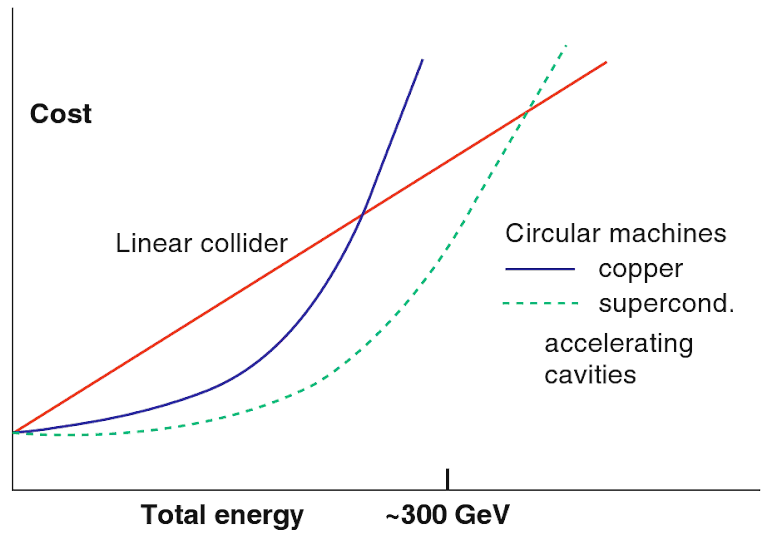
\includegraphics[width=0.55\textwidth]{Figures/Collider_costs.png}
\caption[Construction cost of linear and circular colliders]{Relations between the construction cost and the center-of-mass energy for linear and circular \positron\electron colliders~\cite[p. 13]{Schopper}.}
\label{fig:Costs}
\end{figure}
\chapter{The International Linear Collider}
\label{ILC}
\begin{chapterabstract}
For answering the fundamental questions of mankind, it is necessary to understand the world in great detail.
In order to confirm theories in particle physics, or to disprove them, it is often important to be able to measure the qualities of particles or their interactions to several decimal places.
For measurements in high-energy particle colliders, such precisions can only be reached in linear lepton colliders.
The following sections will present a new design for such a collider on the precision frontier: the International Linear Collider (ILC). 
Its proposed layout, the possible construction sites, the detectors, and the physics motivation for such a capable accelerator will be explained.
\end{chapterabstract}
\newline

The International Linear Collider (ILC) is a proposed linear \positron\electron collider with a center-of-mass energy of \SI{250}{\GeV}, extendable to 350-\SI{500}{\GeV} and possibly even \SI{1}{\TeV}.
Its high luminosity and its state of the art technologies for the detectors and the machine will make the ILC an unprecedented precision machine, complementary to the currently existing high-energy physics accelerators, such as the Large Hadron Collider (LHC) at CERN.
The designs of the collider and the detector concepts are a result of over twenty years of research at over 300 science laboratories and universities all over the world~\cite{TDR1}.
The ILC project is therefore truly an international project.

\section{The ILC layout}
\label{ILC:layout}
The ILC was originally designed to collide electron and positron beams with a center-of-mass energy of \SI{500}{\GeV} in the first stage of operation.
The layout, as well as research results and physics motivations of this \SI{500}{\GeV} machine were summarized in great detail in the Technical Design Report (TDR) in 2013~\cite{TDR}.
Because of political developments and the request in 2017 to reduce the initial construction cost, the first stage collision energy was reduced to \SI{250}{\GeV}.
As it is in the nature of linear accelerators that the beam energy is linearly proportional to the accelerator length, the basic layout of the ILC as stated in the TDR is still the same for the new so-called ILC250.
However, the changes that were made to the layout are given in this section, together with an overview of the generation, preparation and collision of the particle beams in this linear collider concept.
%This is also the reason why the ILC has the possibility to upgrade the machine to higher energies later on.

\subsection{From beam generation to collision}
\label{ILC:layout:details}
\paragraph{Beam sources}
Figure~\ref{fig:ILC_Layout} shows the schematic layout of the ILC.
\begin{figure}
\centering
\includegraphics[width=0.8\textwidth]{Figures/ILC_layout_edited.png}
\caption[Schematic layout of the ILC]{Schematic layout of the ILC~\cite[based on p. 9]{TDR1}}
\label{fig:ILC_Layout}
\end{figure}
The electrons are produced by a GaAs photocathode in a DC electron gun~\cite[p. 13]{TDR32}.
By shining a circularly polarized laser on the electron beam, a beam polarization of at least \SI{80}{\percent} is achived, i.e. more than \SI{80}{\percent} of all electrons have the same handedness\footnote{For a left-handed particle, its spin and its momentum are antiparallel, pointing in opposite directions, and vice versa for a right-handed particle.}~\cite[p. 81]{TDR32}:
\begin{equation}
 P_e = \frac{N_L-N_R}{N_L+N_R} > 0.8
\end{equation}
The electrons from the electron source are captured and continue along the electron beam line.
The beam lines contain several sub-systems that prepare the beams for the main acceleration and the final collision.
One of the first sub-systems of the electron beam line is the initial bunching and pre-acceleration of the beam with normal-conducting RF cavities.
This is done using ``velocity bunching'', as explained in Section~\ref{AccPhysics:Bunching}.
Being pre-accelerated to \SI{76}{\MeV} in this step, the now `bunched' electron beams are accelerated to \SI{5}{\GeV} by a  superconducting booster linac~\cite[p. 81f]{TDR32}.\\
The positron source consists of an undulator and a conversion target~\cite[p. 90f]{TDR32}.
In an undulator, dipole magnets are placed in a line in such a way that their polarity alternates periodically (see Figure~\ref{fig:Undulator}).
For the creation of the positrons, the electron beam is used, which is guided through a \SI{231}{\meter} long helical undulator after being accelerated to the final beam energy of \SI{125}{\GeV}.
Using an undulator with a helical magnetic field causes the electrons to be deflected on a helical trajectory, and to emit synchrotron radiation photons that are circularly polarized\footnote{For circularly polarized light, the field vector of its electromagnetic wave rotates around the direction of propagation.}.
The high-energy photons are then converted in the \SI{7}{\milli\meter} thick titanium-alloy conversion target, where \positron \electron pairs are produced due to pair production.
As the pair production from circularly polarized photons yields longitudinally polarized \positron \electron pairs~\cite{Polarization}, the beam of the captured positrons will have a polarization of at least \SI{30}{\percent}~\cite[p. 14]{TDR32}.
The whole process leads to an effective positron yield of 1.5 positrons per original beam electron passing through the undulator~\cite{Ushakov}.
Due to the fact that the positrons were produced by using an already bunched electron beam, the positron beam is bunched as well. 
\begin{figure}
\centering
\includegraphics[width=0.45\textwidth]{Figures/Undulator_edited.png}
\caption[Schematic layout of an undulator]{Schematic of an electron beam traveling through an undulator with dipole magnets in alternating order~\cite[based on p. 41]{Wille}.}
\label{fig:Undulator}
\end{figure}
\paragraph{Damping rings}
Since the electrons and positrons still have a large emittance from when they originated from their sources, their momentum and beam sizes have to be condensed.
This is done in the damping rings, which have a circumference of \SI{3.2}{\kilo\meter}~\cite[p. 14]{TDR32}.
A layout of the ILC damping rings is shown in Figure~\ref{fig:DR}.
As discussed before, the beams will emit synchrotron radiation when they are deflected in a magnetic field.
This is desired in the damping rings in order to ``cool'' the beams, i.e. to reduce their momenta due to the emission of photons.
The emission of synchrotron radiation happens in the curved sections of the damping rings, but also in the straight sections by the use of wigglers.
Wigglers are similar to undulators, but use fewer magnet pairs and higher magnetic fields.
Charged particles are therefore deflected more in wigglers.
Since the synchrotron radiation photons are emitted tangentially to the beam particle's path, the particle's momentum in the forward direction is reduced.
By accelerating the beams in RF cavities in the straight sections, the beam momentum in the z-direction is increased.
Overall, the momentum in the desired direction rises, whilst the momentum spread shrinks.
\begin{figure}[h]
\centering
\includegraphics[width=0.4\textwidth]{Figures/DR.png}
\caption[Damping ring layout]{Schematic layout of the ILC damping rings.
Next to the injection and extraction system, there are wigglers and RF cavities for the emittance reduction, as well as a chicane for circumference adjustments, and a so-called phase trombone for accommodating changes in the RF phase~\cite[p. 15]{TDR32}.}
\label{fig:DR}
\end{figure}
\\This is, however, not the only effect of damping rings.
As shown in Section~\ref{AccPhysics:Bunching}, the orbit of charged particles in an external magnetic field depends on their momenta.
In the bends, off-momentum particles travel on an orbit with a different radius than particles with the ideal momentum.
Entering the straight sections from suboptimal orbits causes orbit distortions and aberrations in the straight sections, which again causes a rise in the beam emittance.
To counteract this effect, a chicane (see Chapter~\ref{AccPhysics:Bunching}) is needed for adjusting the circumference.
An additional phase trombone system, which consists of sets of alternating quadrupoles, regulates the orbit aberrations due to changes in the RF phase.
Because of the design choice of having a pulse repetition rate of \SI{5}{\hertz}, the beams are stored for \SI{200}{\milli\second} in the damping rings, performing about \num{18000} turns.
After this amount of turns, an equilibrium emittance is reached, and the high quality beam with small beam emittance is extracted and continues along the beam lines.

\paragraph{Bunch compressors}
After passing the damping rings, the electron and positron beams are compressed in bunch length by a two-stage compressor system, using ``magnetic compression''.
Here, the bunch length is reduced from several millimeters to \SI{300}{\micro\meter}.
In both compressor systems, RF cavities are used together with wigglers, which compact the beam momentum by exploiting the momentum spread within the beam bunch.
As discussed in Section~\ref{AccPhysics:Bunching}, the RF frequency and the timing is chosen such that the bunch tail experiences an accelerating phase in the RF cavity, whilst the bunch head experiences a decelerating phase.
The low-momentum particles of the bunch head will therefore be deflected more in the wiggler, whilst the high-momentum particles of the tail are deflected less.
At the end of the compressor system, the particles of the bunch tail and head will have gotten closer, leading to a shortened beam bunch. 
The usage of two separate systems relaxes the requirements a single system would need to fulfill, and allows more flexibility in the operation, e.g. to reduce the beam length below \SI{300}{\micro\meter}~\cite[p. 124]{TDR32}.

\begin{figure}[h!]
\centering
\includegraphics[width=0.4\textwidth]{Figures/Cavity_Gradient.png}
\caption[XFEL cavity gradient]{Maximum and usable gradient distribution of the final European XFEL cavities.
The number of cavities showing a certain gradient is displayed as the bar chart.
The so-called usable gradient is the effective gradient a cavity reaches under strict requirements, such as achieving the operational specification for the quality factor.
The yield, which is shown as the line graphs, is defined as the fraction of cavities which have a gradient higher than the specified value on the x-axis~\cite[p. 18]{XFEL_Cavities}.}
\label{fig:XFEL_cav}
\end{figure}
\paragraph{Main linacs}
Subsequent to bunch compressors, the bunches are injected into the main linear accelerator structures (main linacs).
The two main linacs are designed to accelerate the beams to the final beam energy of \SI{125}{\GeV}, leading to a center-of-mass energy of \SI{250}{\GeV}.
They have a length of \SI{5}{\kilo\meter} each, and use \SI{1.3}{\giga\hertz} superconducting RF cavities with an average accelerating gradient of \SI{31.5}{\mega\volt\per\meter}~\cite{Walker}.
A picture of one of these cavities is shown in Figure~\ref{fig:Tesla_Cavity}. 
Since cavities of the same design are already in use for the European XFEL (X-Ray Free-Electron Laser) at Deutsches Elektronen-Synchrotron (DESY) in Hamburg, their high performance has already been demonstrated~\cite{XFEL}.
The gradient distribution of the cavities used at the European XFEL is shown in Figure~\ref{fig:XFEL_cav}.
The average of the maximum gradient reachable per cavity module is about \SI{35}{\mega\volt\per\meter}, which is higher than the ILC requirements.
This is especially remarkable, as the cavity specifications for the European XFEL are lower than for the ILC.
Another key point is that the production of the cavities is an industrialized process.
The high gradients are therefore not demonstrated in a laboratory environment only, but the gradients are also achieved in a more automated procedure.

\begin{figure}[h!]
\centering
\includegraphics[width=0.6\textwidth]{Figures/BDS.png}
\caption[Layout of the Beam Delivery System]{Schematic layout of the Beam Delivery System (BDS) for the electron beam line.
After the main linac, the BDS for the electron beam line reaches from about Z = -2.2\,km to the Interaction Point (IP) at Z = 0.
The vertical colored lines along the beam line represent the magnets and other devices of the various sub-systems.
Next to diagnostic devices, such as the polarimeter and the energy spectrometer, there are collimation systems to focus and to prepare the beam for the collision at the IP.
The primary dump at Z = 250\,m is the electron beam dump~\cite[p. 135]{TDR32}.}
\label{fig:BDS}
\end{figure}
\paragraph{Beam Delivery System}
The Beam Delivery System (BDS), which has an overall length of about \SI{4.4}{\kilo\meter}, transports the bunches from the linacs to the Interaction Point (IP).
In the BDS, the beams are focused to nanometer size by the Final-Focus (FF) system, which is a crucial part of the ILC program.
Only with nanometer-sized bunches can the ILC can reach luminosities comparable to or beyond the Large Hadron Collider (LHC) at CERN, since the total production cross section for \positron \electron colliders is several orders of magnitude smaller than for proton-proton colliders, such as the LHC, at their respective collision energies (see Figure~\ref{fig:Cross_sections}).
To demonstrate the feasibility of nanometer-scale beams, a test facility was built that is a small scale prototype of the FF system for the ILC: the Accelerator Test Facility (ATF2), which will be presented in more detail in Section~\ref{ATF2}.
The BDS system not only contains the FF system, but also various feedback diagnostics and beam-halo collimators for removing the halo of particles around the beam core in order to reduce the beam background at the IP. 
The sub-system layout for the sophisticated BDS is shown in Figure~\ref{fig:BDS}.
Additionally, shielding systems are installed at various locations along the BDS line, again in order to keep the background level at the IP as low as possible.
Chapter~\ref{BDS_Muons} will talk about muon shielding options that are considered for the ILC.

\paragraph{Beam collision}
After the Final-Focus system, the beams are then finally brought into collision with a crossing angle of \SI{14}{\milli\radian} at the IP.\cite[p. 9-10]{TDR1}
With so-called crab cavities, the bunches are rotated horizontally so that effective head-on collisions are possible.
This is illustrated in Figure~\ref{fig:Crab_crossing}.
The crab cavities are also superconducting RF cavities, but designed for a RF frequency of \SI{3.9}{\giga\hertz} and an accelerating gradient of \SI{5}{\mega\volt\per\meter}~\cite[p. 154]{TDR32}.
The RF phase is modeled in such a way that only the head and the tail of the beam bunch experience acceleration, but in opposite directions.
The voltage needed to rotate a bunch with energy $E_{bunch}$ can be calculated as follows~\cite{Crab_cavities}:
\begin{equation}
 V_{crab}=\frac{cE_{bunch}\theta_C}{2\omega R}
\end{equation}
$\theta_C$ is the crossing angle as before, $\omega$ is the RF frequency of the crab cavity, and $R$ is the ratio of the bunch displacement at the IP to its divergence, i.e. the ratio of the spatial shift at the IP to the increase in the beam size.
With all other quantities fixed, only $R$ can be increased in order to reduce the required voltage.
Therefore, the crab cavities are positioned at locations where this ratio $R$ between the spatial shift and the beam size increase is calculated to be large.
For the ILC, it was calculated that the crab cavities should be located \SI{13.4}{\meter} up- and downstream of the IP~\cite[p. 154]{TDR32}.
\begin{figure}
\centering
\includegraphics[width=0.4\textwidth]{Figures/Crab_crossing.png}
\caption[Schematic of a beam crossing with crab cavities]{Schematic of a beam crossing with crab cavities. In a crossing with crossing angle $\theta_C$, head-on collisions are only possible with crab cavities that rotate the beam in the horizontal plane.}
\label{fig:Crab_crossing}
\end{figure}

\paragraph{Beam parameters}
Table~\ref{tab:ILC_parameters} shows the beam parameters for the baseline design at \SI{250}{\GeV} center-of-mass energy, and for the energy and the luminosity upgrade stages.
%\multicolumn{1}{>{\centering}p{1.5cm}}{\textbf{Baseline 500}} & \multicolumn{1}{>{\centering}p{1.5cm}}{\textbf{Lumi Upgrade}} & \multicolumn{1}{>{\centering}p{1.5cm}}{\textbf{TeV Upgrade}} & {\centering\textbf{LHC 25ns}} \\ 
\begin{table}[h]
\caption{Beam parameters for different phases in the ILC operation scenario (ILC250, ILC500, Luminosity Upgrade, TeV Upgrade)~\cites[p. 11]{TDR1}{CR-0016} in comparison to LHC Run 2 beam parameters~\cites[p. 3ff]{LHC_TDR}{LHC_Parameters}.}
\label{tab:ILC_parameters}
\centering
\begin{tabularx}{0.99\textwidth}{lll|rrrrg}
\hline\hline
& && \multicolumn{1}{>{\centering}p{1.5cm}}{\textbf{ILC250}} & \multicolumn{1}{>{\centering}p{1.5cm}}{\textbf{ILC500}} & \multicolumn{1}{>{\centering}p{1.5cm}}{\textbf{Lumi Up}} & \multicolumn{1}{>{\centering}p{1.5cm}}{\textbf{TeV\\Up}} & \multicolumn{1}{>{\centering}p{1.5cm}}{\textbf{LHC 25ns}}\\
\hline
\cline{1-8}
\hline
E$_{CM}$  &{\small Center-of-mass energy}&{\small(\si{\GeV})}& 250 & 500  & 500  & \num{1000} & \num{14000}\\
n$_b$ &{\small Number of bunches}&& \num{1312} & \num{1312} & \num{2625} & \num{2450} & \num{2808} \\
$f_{rep}$ &{\small Pulse repetition rate}&{\small(\si{\hertz})} & 5 & 5  & 5   & 5 & \num{11245}\\
$\Delta t_b$ &{\small Bunch seperation}&{\small(\si{\nano\second})} & 554 & 554  & 366   & 366 & 25\\
N &{\small Bunch population}&& 2.0$\cdot10^{10}$ & 2.0$\cdot10^{10}$  & 2.0$\cdot10^{10}$  & 1.74$\cdot10^{10}$ & 11.5$\cdot10^{10}$\\
q$_b$ &{\small Bunch charge}&{\small(\si{\nano\coulomb})}  & 3.2 & 3.2  & 3.2  &  2.7 & 18.4  \\
$\sigma_x^*$ &{\small Horiz. beam size at IP}&{\small(\si{\nano\metre})} & 515.5 & 474  & 474  &  481 & \num{16700}\\
$\sigma_y^*$ &{\small Vert. beam size at IP}&{\small(\si{\nano\metre})} & 7.7 & 5.9 &  5.9  &  2.8 & \num{16700}\\
$\sigma_z$ &{\small Longit. beam size}&{\small(\si{\milli\metre})} & 0.3 & 0.3  &  0.3  &  0.25 & 0.755\\
L &{\small Luminosity}&{\small(\si{\per\centi\metre\squared\per\second})} & 1.35$\cdot10^{34}$ & 1.8$\cdot10^{34}$ & 3.6$\cdot10^{34}$ &3.6$\cdot10^{34}$ & 1.0$\cdot10^{34}$\\
\hline\hline
\end{tabularx}
\end{table}
For all ILC running scenarios, the beam sizes are several orders of magnitude smaller than for the LHC Run 2, which is the reason for the comparable luminosities as mentioned above.
Despite the number of bunches per pulse and the bunch population being smaller, the LHC luminosity can be exceeded.
It is striking that the beam sizes in the horizontal and vertical plane are symmetric for the LHC, whereas they are different for the ILC.
This is a design choice, reducing the effect of beamstrahlung whilst enhancing the luminosity.
As shown in Equation~\ref{eq:pair_number}, the number of background particles from beamstrahlung is inversely proportional to the sum of the beam sizes, $\sigma_x+\sigma_y$.
At the same time, the luminosity is inversely proportional to the product of the beam sizes, $\sigma_x\cdot\sigma_y$, as shown in Equation~\ref{eq:luminosity} in Chapter~\ref{AccPhysics:Linear-Circular}.
By choosing the beam sizes to be $\sigma_x\gg\sigma_y$, the product is small leading to large luminosities, while the sum is large leading to a diminished background rate.

\paragraph{Interaction region and beam dumps}
The Interaction Region (IR) houses the two detectors for the ILC: the Silicon Detector (SiD) and the International Large Detector (ILD), which are in a so-called ``push-pull'' system.
The detectors and the push-pull system are explained in more detail in Section~\ref{ILC:detectors}.\\
Finally, after collision the spent beams are guided through the extraction line towards the main beam dumps, where they are dumped.
The current designs for the main beam dumps are based on a water tank, using high-pressure water with velocity flow systems.
Since the water tanks are designed to be sufficient for all energy and luminosity stages, they are supposed to withhold a particle beam with a beam power of \SI{14}{\mega\watt} for the \SI{1}{\TeV} operation~\cite[p. 18]{TDR32}.
This leads to high irradiation of the beam dump surrounding and dangerous conditions for maintenance staff.
In Chapter~\ref{BeamDumps}, which talks about the simulation of the main beam dumps done for this thesis, more details are given for the current beam dump designs.

\subsection{Staging}
\label{ILC:layout:staging}
As mentioned above, the panel of the International Committee for Future Accelerators (ICFA) officially decided in 2017 to reduce the center-of-mass energy of the first ILC stage to \SI{250}{\GeV}, in order to reduce the total costs of the ILC project.
ICFA's official statement declares that the ``[...] International Linear Collider (ILC) operating at 250 GeV center-of-mass energy will provide excellent science from precision studies of the Higgs boson.
Therefore, ICFA considers the ILC a key science project complementary to the LHC and its upgrade.
ICFA welcomes the efforts by the Linear Collider Collaboration on cost reductions for the ILC [...]''~\cite{ICFA_Statement}.\\
The total costs for realizing the ILC includes the manpower, the costs for the construction of the so-called conventional facilities, such as the underground tunnels and the surface buildings, and the costs for the production and assembling of the accelerator and detector components.
When breaking the total costs down into the subsystems, then the conventional facilities together with the production of the RF modules for the main linacs make up almost \SI{75}{\percent} of the total costs~\cite[p. 20f]{TDR1}.
These estimations are based on cost inquiries with several industrial companies, as well as on experiences collected at other accelerator projects, such as the European XFEL which uses the same design for the RF cavities as planned for the ILC.\\
Regarding the ILC layout, several options are under discussion which are shown in Figure~\ref{fig:Staging}.
These options would yield a cost reduction of up to \SI{34}{\percent}~\cite{Cost_reduction}, resulting in about \SI{66}{\percent} of the initial costs for the \SI{500}{\GeV} machine by reducing the length of the tunnel (options A, B, and C), or by additionally reducing the number of RF cavities (options A', B' and C').
In options A', B', and C', the RF cavities are planned to have a larger accelerating gradient so that a smaller number of cavities would still lead to the same beam energy as for options A, B, and C.
Overall, option A' foresees the shortest possible tunnel for \SI{250}{\GeV} and the smallest number of cavities, and therefore results in the highest cost reduction.\\
As explained before, the costs for the tunnel and the accelerating structures represent indeed the largest fraction of the total costs, and will be reduced by the staging options.
However, the other parts of the accelerator and the surface buildings will not change by the staging scenarios but form basic costs because of which the maximum cost reduction cannot exceed \SI{34}{\percent}.
Therefore, it has to be considered whether the cost cutback of option A' outweighs all other options with a tunnel length suitable for an energy upgrade.
An extended tunnel would give a positive sign to the ILC community that an energy upgrade is definitely foreseen for the future.
\\Figure~\ref{fig:ILC_runningtime} shows two possible running scenarios for the staged ILC.
In both cases, the ILC will have energy and luminosity upgrades, so that it will reach the same integrated luminosity over a different amount of time.
On the left hand side, the plot shows an expected operation time of 15 years for the ILC250 with a luminosity upgrade at the midway-point.
As shown in Equation~\ref{eq:luminosity}, the luminosity of a particle collider is directly proportional to the number of bunches colliding in every beam pulse.
Hence, by increasing the number of bunches by a factor of two, the luminosity for the luminosity upgrade stage is doubled.
After an energy upgrade by extending the main linacs, the operation at \SI{500}{\GeV} and a short run at \SI{350}{\GeV} for dedicated measurements of the top quark qualities would be possible.
The overall operation time would stretch out to 26 years.\\
For the second scenario on the right hand side of Figure~\ref{fig:ILC_runningtime}, it was assumed that the beam parameters are changed in such a way that the beam is more strongly focused at the IP and therefore that the instantaneous luminosity is enhanced.
This shortens the operation time of the ILC250 stage to 11 years, and the overall run time to 22 years, whilst still achieving the same integrated luminosity~\cite[p. 7]{PhysicsCase}.
\begin{figure}
\centering
\includegraphics[width=0.9\textwidth]{Figures/Staging.png}
\caption[Different layouts for the ILC250 stage]{Different layouts for the ILC250 stage.
The original layout has foreseen a tunnel fitting linacs for \SI{250}{\GeV} beam acceleration, which would lead to a center-of-mass energy of \SI{500}{\GeV}.
For the new stage, the linacs are reduced in length.
The discussions about the layout involves also the length of the tunnel.
Option B and C would foresee longer tunnels that would facilitate a later energy upgrade to 350 or \SI{500}{\GeV}.\\
Options A', B' and C' correspond to options A, B and C regarding the tunnel length, but they assume RF cavities with a gradient of \SI{35}{\mega\volt\per\meter} instead of \SI{31.5}{\mega\volt\per\meter} in order to reduce the number of cavities needed~\cite[p. 19]{Staging}.}
\label{fig:Staging}
\end{figure}
\begin{figure}[htbp]
\centering
\includegraphics[width=0.98\textwidth]{Figures/ILC_runningtime.png}
\caption[ILC run plan]{Two possible ILC run plans for the staged ILC~\cite[p. 8]{PhysicsCase}.}
\label{fig:ILC_runningtime}
\end{figure}

\section{Possible site}
Out of originally more than ten potential ILC sites in Japan, the Kitakami mountains in the Tohuku Prefecture were chosen as the preferred site for the ILC~\cite{Site}.
This decision was made in August 2013 after a detailed study of all site specific factors, like the geological conditions, the infrastructure, and the impact on the environment and the economy.
Measurements of the Kitakami mountains have shown that it consists mostly of granite rock with the best qualities for the ILC, with respect to vibration and rock stress.
As can be seen in Figure~\ref{fig:ILC_Site}, the closest city (with about 120,000 citizens) would be Ichinoseki.
Morioka and Sendai are the biggest cities close to the candidate site, with Tokyo being about \SI{430}{\kilo\meter} away.
Although being in the north of Japan, the travel time from Tokyo is only about three hours by Shinkansen, Japan's high-speed bullet train, and the proximity to the coast line allows the transportation of construction, machine, and detector parts by ship.
Additionally, there are local airports in both, Morioka and Sendai, presenting further options for traveling and the transportation of construction materials.
\label{ILC:site}
\begin{figure}[h]
\centering
\includegraphics[width=0.6\textwidth]{Figures/ILC-site.png}
\caption[Possible site for the ILC]{The possible site for the ILC is the Kitakami mountains in the Tohuku prefecture.\cite{Kitakami}}
\label{fig:ILC_Site}
\end{figure}

\section{Physics motivation}
\label{ILC:physicsmotivation}
After having shown that the ILC as a linear lepton collider is designed to be a state-of-the-art precision machine, this section will present its physics goals.
With the LHC as a machine at the energy frontier, the ILC will be a complementary collider aiming rather for much needed precision than for searching for new particles at high energies.
The ILC therefore intends to find new particles and new physics through highest precision measurements.
It is often called the future Higgs factory which will measure the qualities of the Higgs boson with much higher precision than has been done so far.
Additionally, the different stages of the ILC will also measure the top quark qualities, and will have access to Beyond Standard Model (BSM) physics.
Since the first ILC stage will run at a center-of-mass energy of \SI{250}{\GeV}, this section will focus more on the measurements of the Higgs boson than of the top quark and the BSM physics.
 
\subsection{How to get there}
To reach the precision the ILC promises, it must achieve four different objectives.
These objectives are all linked so that one is dependent on the others.
In the following section, these four objectives of the ILC are explained in comparison to the LHC.

\paragraph{Minimal background}
Due to leptons in the initial state, there will be one physics process per colliding lepton pair.
Leptons are elementary and not composite particles like the proton, therefore there are no underlying events which arise from other partons of the composite particle.
The energy range of the final state particles is restricted, since the initial energy of the colliding beams can be set precisely and only point-like particles collide.
By adjusting the center-of-mass energy of the collision and running threshold scans at the mass of the particle of interest, the rate of the desired process can be increased.
This is only possible at lepton colliders.
\\Beam polarization contributes to the small background levels as well, since the polarization can be set in such a way that weak interactions are either enhanced or suppressed.
As the weak interaction acts only on left-handed fermions, the polarization (or handedness) of the beam particles has an effect on the processes that can occur.
This effect can be seen directly by looking at the two possible production modes at an \positron\electron collider (see also Chapter~\ref{Production_modes}):
direct \positron\electron annihilation, and \positron\electron scattering.
In the SM annihilation process, the electron and positron have to be of opposite handedness due to the nature of weak interactions.
The annihilation cross-section can therefore be enhanced by polarizing the beams to have opposite polarization.
For the \positron\electron scattering process, the handedness of the final state particles is dependent on the handedness of the incoming particles.
By setting different polarization combinations, the properties of the final state particles, the interactions, and the couplings can be studied. %Check out PhD Thesis of Annika Vauth, p.10-12
Therefore, depending on the physics process of interest, the polarization can enhance the signal whilst suppressing the background. 
\\Figure~\ref{fig:Cleanliness} shows two event displays of a Higgs event at the LHC and the ILC in comparison.
Due to the nature of composite particles, event displays at the LHC are dominated by underlying events and pileup events.
At the ILC, the event displays are clean, and the tracks from the final state particles of the physics event can be distinguished easily.
\begin{figure}
\centering
\includegraphics[width=0.6\textwidth]{Figures/Cleanliness.png}
\caption[Clean environment at the ILC]{Comparison of the event displays of a Higgs event at the  LHC and at the ILC~\cite[based on p. 4]{ILCPhysics_Thomson}.
At the LHC, underlying events and pileup events populate the detector, whilst at the ILC the hits are mainly from the final state particles of the physics interaction of interest.
}
\label{fig:Cleanliness}
\end{figure}

\paragraph{Democratic particle cross sections}
Because the elementary coupling of Z bosons and photons is of the same order for all quarks and leptons, the \positron\electron annihilation produces pairs of all species at similar rates.
In addition, the ILC will record all events without triggers.
This means that no process will be rejected, and the complete readout of all events measured with the detectors will be stored for later analysis.
This is only possible because the total number of detector hits from background events is small.
Small background levels therefore imply small detector occupancies.

\paragraph{Small uncertainties}
The initial state of all events is precisely known, both in terms of the particles undergoing the interactions and also the energies involved in the initial states.
Additionally, there are only events with couplings to electroweak interactions, so that PDF uncertainties and systematic uncertainties due to QCD corrections are omitted.
\\The small uncertainties enhance theoretical and experimental precisions at \positron\electron colliders.

\paragraph{Complete knowledge}
Because of the small background and the possibility to record and store the complete detector readouts, processes can be reconstructed in completeness without theoretical assumptions.
The quark and lepton momenta can therefore be determined by kinematic fits.
Studies of the spin-dependence of the production and decay processes are also possible.\\
Due to the high energy resolution and the fact that the initial particle energies are precisely known, particles with small mass differences are distinguishable, i.e. peaks in mass spectra that are close together are more likely to be separable.
That means that new particles might indeed be found at the ILC.\\
Additionally, c-tagging will be a possible tool for physics analyses, and will improve many physics studies at the ILC.
The life time of a charm quark (c) before it hadronizes is around \SI{80}{\micro\meter}, which is a perfect way to identify that a charm quark was involved in the event.
Since the distance between the primary and the secondary vertex can only be measured by a vertex detector with micrometer resolution, c-tagging is in general very difficult.
However, it will be possible at the ILC, because the detector concepts foresee such a resolution, and the nanometer-sized beam allows the inner vertex detector radius to be very close to the interaction point.
%only approximately \SI{10}{\milli\meter}. 
%charm hadron lifetime: 80microns, bottom hadron lifetime: 400microns

\subsection{ILC as a Higgs factory}
The ILC250 stage will be a so-called Higgs factory, tuned to a center-of-mass energy of \SI{250}{\GeV}, where the cross section $\sigma$ for Higgs production is at its maximum.
Due to the large luminosity and the capability for precision measurements, as has been shown in the section above, the individual Higgs boson qualities can be measured to a percent accuracy in a completely model independent way.
These Higgs boson properties include the Higgs mass, its couplings to Standard Model particles, as well as its total decay width.
In contrast, for the LHC experiments, global fits to all Higgs signals together with theoretical assumptions of its decay width is the only way to gain the Higgs couplings.
\\After a brief overview of the Higgs production modes and the determination of the Higgs properties at the ILC, it will be shown how the unprecedented precisions are achievable at the ILC.

\subsubsection{The Higgs production modes at an \positron\electron collider}
There are three main production modes for Higgs bosons at an \positron\electron collider, such as the ILC.
As can be seen in Figure~\ref{fig:HiggsProduction}, the largest contribution to the overall production cross section is the Higgsstrahlung process, where a Higgs boson is produced in association with a Z boson ($e^+e^-\rightarrow Zh$).
In vector boson fusion (VBF) processes, like the WW fusion and the ZZ fusion, the fusion of two bosons produces a Higgs boson and a pair of leptons.
For the WW fusion, an electron-neutrino and its anti-neutrino are produced ($e^+e^-\rightarrow \nu\bar{\nu} h$), whilst for the ZZ fusion it is an electron and a positron ($e^+e^-\rightarrow e^+e^-h$).
The production cross sections for these processes as a function of the center-of-mass energy behave quite differently:
The dominant process at energies between 200 and \SI{450}{\GeV} is the Higgsstrahlung process, replaced by the WW fusion process above \SI{450}{\GeV}.
The ZZ fusion cross section contributes the least, with less than \SI{10}{fb}.
It is suppressed, since the couplings of the neutral current are smaller than the charged current couplings.\\
As te cross section of the Higgsstrahlung process peaks at \SI{250}{\GeV}, the ILC250 stage will mainly use this production mode for the precision measurements of the Higgs boson qualities.
At \SI{250}{\GeV}, the ILC will provide an even more precise measurement of the Higgsstrahlung cross section and hence of the branching ratios of the various decay modes of the Higgs boson than at a center-of-mass energy of \SI{500}{\GeV}~\cite[p. 14]{PhysicsCase}.
This is true despite the lower luminosity at \SI{250}{\GeV}, due to the larger cross section and the smaller background occupancy of the detectors (see Chapter~\ref{PairBkg:occupancy}).
\begin{figure}
\centering
\includegraphics[width=0.5\textwidth]{Figures/HiggsProductionCrossSection.png}
\caption[Cross section for the Higgs production modes at ILC]{Cross sections for the Higgs production modes at the ILC, with beam polarization of 80\,\% for the electron and 30\,\% the positron beam~\cite[p. 13]{PhysicsCase}.
The three main processes are ZZ fusion, WW fusion, and Higgsstrahlung.}
\label{fig:HiggsProduction}
\end{figure}

\subsubsection{The Higgs measurements}
To know the Higgs couplings to Standard Model (SM) particles as precisely as possible is one of the most important goals for the ILC.
Many theories about particles beyond the SM predict deviations from the SM couplings at the \SI{1}{\percent} level.
Therefore, if these theories prove to be true, only with the highest precisions could a new particle be discovered, and a different model beyond the Standard Model be acknowledged.
\\As shown in the section above, the Higgsstrahlung production mode presents a prominent way to measure the Higgs boson properties.
Due to the accurate knowledge of the initial state particles (the colliding electron and positron) and their energies, the unambiguous reconstruction of the Z boson recoiling against the Higgs boson makes the identification of the Higgs possible without the need to reconstruct its decay particles.
This so-called recoil method to identify the Higgs independently of its decay channels therefore allows a model independent way to determine the Higgs mass, its total decay width, the branching ratios, and the Higgs couplings. 
The high precision of the Higgs measurements will furthermore be a result of the high luminosity of the ILC and of the peak cross section of the Higgsstrahlung mode.

\paragraph{Higgs mass}
To gain the recoil mass of the Higgs boson, the difference in the four-momenta between the Z boson decay particles and the initial state particles has to be calculated~\cite[p. 7]{ILCPhysics}:
\begin{equation}
 m_{recoil}^2=(P_{ini}-(P_{f+}+P_{f-}))^2
\end{equation}
$P_{ini}$ is the sum of the four-momenta of the initial state particles, $P_{f+}$ and $P_{f-}$ are the measured four-momenta of the fermionic decay products of the Z boson.\\
Higgsstrahlung events with the Z boson decaying into two leptons, especially muons, are the cleanest events, reaching the highest precisions of the Higgs measurements due to the high-resolution tracking detectors and the muon-veto system of the detector concepts.
By counting such events, the full Higgsstrahlung cross section $\sigma(e^+e^-\rightarrow Zh)$ can be determined to a \SI{1}{\percent} precision~\cite[p. 12]{PhysicsCase}.


\paragraph{Higgs decay width}
The total decay width $\Gamma_{h,tot}$ can be measured through~\cite[p. 14]{PhysicsCase}:
\begin{equation}
 \Gamma_{h,tot}=\frac{\Gamma(h\rightarrow XX)}{BR(h\rightarrow XX)}
\end{equation}
where $\Gamma(h\rightarrow XX)$ is the partial decay width, specific for the Higgs decay to any SM particle X, and $BR(h\rightarrow XX)$ is the corresponding branching ratio.\\
The branching ratios are calculated by first measuring the rates of the occurring decay channels.
A branching ratio of a certain decay channel is then determined by dividing the measured event rate by the production cross section, since event rates are given as $\sigma\cdot BR$.
Due to the high precision measurement of the Higgsstrahlung cross section, as discussed in the paragraph above, the branching ratios can be calculated equally precisely.
Figure~\ref{fig:HiggsBR} shows the branching ratios of the Higgs boson as a function of the Higgs mass.
\begin{figure}
\centering
\includegraphics[width=0.5\textwidth]{Figures/Higgs_BR.png}
\caption[Higgs decay branching ratios]{Branching ratios of the Standard Model Higgs decay channels, as a function of the Higgs mass~\cite[p. 15]{TDR2}.}
\label{fig:HiggsBR}
\end{figure}
%Since $h\rightarrow WW^*$ has a large branch ratio for the known Higgs mass of \SI{125}{\GeV}, this process can be measured with high precision, and is therefore used for the calculation of the total Higgs decay width.
\\The partial decay width of a given decay is measured as the resonance width in the mass spectrum of the decay particles.
However, the decay width $\Gamma(h\rightarrow ZZ^*)$ can be gained through the relation~\cite[p. 14]{PhysicsCase}:
\begin{equation}
 \Gamma(h\rightarrow ZZ^*)\propto g^2_{hZZ} \propto \sigma(e^+e^-\rightarrow Zh)
\end{equation}
with the Higgsstrahlung production cross section, and the Higgs coupling $g_{hZZ}$ to the Z boson. 
%TODO: How is the partial decay width calculated through this equation exactly?
\\Finally, by combining the branching ratio with the partial decay width, the total Higgs width is determined in a model independent way without theoretical assumptions, since both the branching ratio and the partial width were measured independently of the Higgs decay channels.

\paragraph{Higgs couplings}
The coupling of the Higgs boson to any Standard Model particle X is given with the notation $g_{hXX}$, and expresses the strength of the interaction between the Higgs and particle X.
This coupling constant is involved in both the Higgs production and its decay, and is hence a dependency of the production cross sections as well as of the decay branching ratios.\\
The dependence between the coupling constant and the cross section for the Higgsstrahlung, for instance, is given as~\cite[p. 4]{PhysicsCase_Junping}:
\begin{equation}
 \sigma(e^+e^-\rightarrow Zh)=F_1\cdot g^2_{hZZ}
\end{equation}
where $F_1$ is a parameter that can be calculated unambiguously from the Feynman diagram for this process.
$g_{hZZ}$ can therefore be determined with high precision, comparable to the precision of the Higgsstrahlung cross section determination itself.\\
All other couplings however are gained via the partial decay width $\Gamma$, which is calculated through the total Higgs width and the various branching ratios:
\begin{equation}
 g^2_{hXX}\propto\Gamma(h\rightarrow XX)=\Gamma_{h,tot}\cdot BR(h\rightarrow XX)
\end{equation}
The precision on the couplings is directly dependent on how accurately the full process can be measured and recorded.
As explained above, the reconstruction of complete events at the ILC with its low background occupancies enables a \textit{model independent} determination of the Higgs boson qualities.
The recoil method to gain the full Higgsstrahlung cross section allows the calculation of the Higgs branching ratios and the total decay width without theoretical assumptions.
In contrast to that, due to large background levels and therefore high detector occupancies in hadron colliders, specific processes are not easily distinguishable from background events.
Additionally, the main Higgs production mode at hadron colliders is gluon-gluon fusion, which is open to processes beyond the Standard Model.
These are the reasons why LHC experiments can not measure the full Higgs cross section without \textit{model dependent} assumptions, which is the key to a model independent determination Higgs properties.\\
This leads to differences in the relative Higgs boson coupling precisions of a factor of up to 10 between High-Luminosity LHC (HL-LHC) and ILC results, as can be seen in Figure~\ref{fig:Higgs_couplings}.
The ILC250 will deliver Higgs coupling precisions to a percent level.
As discussed above, the coupling to the Z boson can be measured with such high accuracy that even in the initial ILC250 run a precision of about \SI{0.75}{\percent} can be achieved~\cite[p. 6]{HiggsCouplings_Junping}.
After an upgrade to a center-of-mass energy of \SI{500}{\GeV}, the precisions for all couplings will improve by at least a factor of two.
When comparing the coupling precisions achieved through model dependent fits of the High-Luminosity LHC (HL-LHC) to precisions achieved at the ILC (see Figure~\ref{fig:Higgs_couplings_b}), the differences between the two machines become clear.
Nevertheless, a synergy of the data collected at both machines is beneficial for the Higgs coupling to photons for instance.
The combined knowledge reduces the relative precision from a few percent to below \SI{1}{\percent} precision.
%\begin{figure}[h]
%\centering
%\includegraphics[width=0.6\textwidth]{Figures/Higgs_couplings.png}
%\caption[Higgs coupling precisions]{Comparison of the precision reached at the ILC and at the High-Luminosity LHC (HL-LHC) for couplings g(hXX) of the Higgs boson (h) to SM particles (X)~\cite[p. 17]{PhysicsCase}.\\
%The plot shows the relative precisions for the Higgs couplings calculated from the \textbf{model dependent} fits to simulated data from the HL-LHC, and from these fits combined with \textbf{model independent} fits to simulated data from the ILC.}
%\label{fig:Higgs_couplings}
%\end{figure}
 \begin{figure}[h]
 \centering
  \begin{subfigure}[b]{0.49\textwidth}
   \centering
    \includegraphics[width=\textwidth]{Figures/Higgs_couplings_modelindependent.png}
   \caption{Model independent analysis}
   \label{fig:Higgs_couplings_a}
   \end{subfigure}
   \hfill
    \begin{subfigure}[b]{0.49\textwidth}
   \centering
    \includegraphics[width=\textwidth]{Figures/Higgs_couplings_modeldependent.png}
   \caption{Model dependent analysis}
   \label{fig:Higgs_couplings_b}
   \end{subfigure}
   \caption[Higgs coupling precisions]{Comparison of the precision reached at the ILC and at the High-Luminosity LHC (HL-LHC) for couplings g(hXX) of the Higgs boson (h) to SM particles (X), here named as $\kappa_X$~\cite{HiggsCouplings_Junping}.\\
   Plot (a) shows the relative precisions for the Higgs couplings calculated from \textbf{model independent} fits to simulated data from the ILC with different center-of-mass energies.
   Plot (b) shows the Higgs coupling precisions calculated from \textbf{model dependent} fits to simulated data from the HL-LHC in comparison to simulated data from the ILC.}
   \label{fig:Higgs_couplings}
 \end{figure}
 
\subsection{Physics at later ILC stages}
The ILC physics program has an excellent discovery potential for new physics.
The first stage at \SI{250}{\GeV} has the capability to make a prominent progress in the Higgs sector by measuring the Higgs branching ratios to highest precisions.
The later stages will complete this picture: 
precision measurements of the top quark, further Higgs measurements, and BSM searches will be accessible at \SI{350}{\GeV}, \SI{500}{\GeV}, and possibly \SI{1}{\TeV}.
\\The ILC350 will enable a threshold scan of $t\bar{t}$ production in order to measure the top quark mass and its total decay width to unprecedented accuracy.
The Higgs coupling to the top can be derived from precision cross section measurements of these processes.
Since the top quark is the heaviest known elementary particle, it is expected to have the strongest coupling in the Higgs sector.
Therefore, its mass and its coupling to the Higgs boson are important quantities in many particle physics theories, and will be measured in a model independent manner as described in the section above.
\\At a center-of-mass energy of \SI{500}{\GeV}, further improvements in the precision measurements of the Higgs boson properties can be achieved.
As has been shown in Figure~\ref{fig:Higgs_couplings}, the Higgs coupling precisions will be reduced by a factor of two.
Only with such precisions, can deviations from Standard Model predictions be discovered, which has implications for new physics beyond the Standard Model.
Additionally, measuring the Higgs self-coupling in multi-Higgs production processes is another goal of the ILC500.
\\In all stages, the discovery potential in precision measurements is considerably improved.
This includes searches for dark matter, supersymmetry (SUSY), and further beyond the Standard Model theories.
An overview of the physics motivation for higher ILC stages can be found in~\cite{PhysicsCase}.

\section{The experiments}
\label{ILC:detectors}
Previous sections have shown that the physics goals of the ILC are based on precision measurements that heavily rely on an outstanding detector performance in order to achieve the promised goals.
The performance requirements are accordingly strict, and the detectors are designed to fulfill them for the full energy range of operation.
Some of the requirements are: exceptional energy and spatial resolution, vertex recognition, and reliable flavor tagging.
Additionally, the detector designs have to address the background arising from beam-beam interactions and the accelerator itself, which is explained in Chapter~\ref{Backgrounds}.
Especially the forward detector systems have to be radiation hard to avoid radiation damage.
All these requirements are fulfilled in the design of the two ILC experiments.
\\In order to preserve competitive spirit and the ability to cross-check results, the ILC has two detectors despite the fact that it is a linear and not a circular collider.
The so-called push-pull system makes this possible by allowing the detectors to switch position after a certain amount of data-taking time.
The whole detector together with the last quadrupole magnet of the accelerator Final-Focus system will be pulled out of the beam line, and the other detector takes its place.
The whole process is designed to take from several hours up to 1-2 days, but involves some challenges especially for the magnets, the cryogenics, and the detector and machine alignment~\cite[p. 28-29]{TDR1}.
The two detectors, the Silicon Detector (SiD) and the International Large Detector (ILD), will be explained in detail in the following sections.
The focus will lie on SiD, since all the background studies presented in this thesis were done in the context of the SiD detector.

\subsection{The Silicon Detector}
\label{ILC:SiD}
The SiD is designed to be a robust, compact detector.
Its vertex and tracker system, as well as the electromagnetic calorimeter (ECAL) are purely based on silicon sensors.
The silicon design, in comparison to other designs for the vertex and tracking detectors, is more robust regarding the beam background and timing~\cite[cf. p. 57ff]{TDR4}.
\\Being designed to be compact, the measurements for the full detector are \SI{14}{m} in height and \SI{11}{m} in length.
To compensate the small radius, the magnetic field of the superconducting solenoid magnet is \SI{5}{T}, so that SiD is hermetic and contains the full particle showers.
The detector is optimized for Particle Flow Algorithms (PFA), in order to improve on the jet energy reconstruction capability.
PFA is a reconstruction method that reconstructs each particle of the final state individually and uses the different subdetectors for a specific purpose.
Therefore, charged particles are reconstructed from tracks in the tracker device.
The electromagnetic calorimeter (ECAL) is used for photons, and the electromagnetic (ECAL) and hadronic calorimeter (HCAL) together for other neutral particles~\cite{PFA}.
\\Table~\ref{tab:KeyParametersSiD} lists the key parameters and measurements of the SiD subdetector systems together with the technologies for the individual sub-systems.
Additionally, Figure~\ref{fig:SiD} shows a visualization of the SiD detector and its subdetectors, which will be explained in the following paragraphs.
A more detailed description can be found in~\cite{TDR4}.
\begin{figure}[h]
\centering
\includegraphics[width=0.8\textwidth]{Figures/SiD_new.jpg}
\caption[Visualization of the SiD detector]{The SiD detector consists of the vertex and tracking detectors (red), the electromagnetic calorimeter (ECAL) (green), the hadronic calorimeter (HCAL) (purple) and the muon system (gray).
All subdetectors except the muon system are inside the solenoid magnet.
Outside the muon endcaps is the detector specific background shielding, called ``Pacman'' with an inner (light gray) and an outer (beige) layer~\cite{SiD_Geo}.}
\label{fig:SiD}
\end{figure}

\begin{table}[h!]
\caption[Key parameters of the baseline SiD design]{Key parameters and technologies foreseen for the baseline SiD design. All dimensions are given in cm~\cite{SiD_Geo}.}
\label{tab:KeyParametersSiD}
\centering
\begin{tabularx}{0.81\textwidth}{l|llll}
\hline\hline
SiD Barrel & Technology & Inner radius & Outer radius & z extent\\
\hline
Vertex detector & Silicon pixels & 1.4 & 6.0 & $\pm 6.3$ \\
Tracker & Silicon strips & 21.5 & 121.5 & $\pm 150.3$ \\
ECAL & Silicon pixels-W & 126.5 & 140.3 & $\pm 176.5$ \\
HCAL & SiPM-steel & 140.3 & 256.8 & $\pm 295.0$ \\
Solenoid & 5 T SC & 260.4 & 342.9 & $\pm 295.0$ \\
Muon System & Scintillator-steel & 345.4 & 605.4 & $\pm 416.0$ \\
\hline
SiD Endcap & Technology & Inner z & Outer z & Outer radius\\
\hline
Vertex detector & Silicon pixels & 7.3 & 83.4 & 7.1 \\
Tracker & Silicon strips & 77.0 & 164.3 & 125.5 \\
ECAL & Silicon pixel-W & 165.7 & 180.0 & 126.5 \\
HCAL & SiPM-steel & 180.5 & 300.0 & 140.3 \\
Muon System & Scintillator/steel & 300.0 & 560.0 & 605.4 \\
LumiCal & Silicon-W & 155.7 & 169.55 &  20.0 \\
BeamCal & Semiconductor-W & 326.5 & 344 & 14.0 \\
\hline\hline
\end{tabularx}
\end{table}

\newpage
\paragraph{Vertex detector}
The vertex detector, shown in Figure~\ref{fig:SiD_VXD}, will be the inner most subdetector with the measurements of a soda can.
With its five layers for the barrel and the endcaps, it will be able to do very precise measurements.
The requirements for the vertex detector performance are very demanding:
The spatial resolution with less than \SI{5}{\micro\meter} allows very precise tracking, whilst the impact parameter resolution is aimed for about \SI{3}{\micro\meter} for the verification of the primary vertex, as well as of the secondary vertex of a bottom quark (b-tagging) and even of a charm quark (c-tagging).
The latter is very challenging due to the short flight distance of the charm quark of only a few microns before it hadronizes.
Additionally, a very small material budget of about \SI{0.1}{\xzero} is foreseen for the vertex detector in order to limit particle showers and multiple scattering in this subdetector~\cite{SiD_Update}.
To achieve this minimal material budget, sensor technologies are considered that foresee the implementation of the sensor buffers on the chips directly to minimize the used material. 
For a comparison to the CMS pixel detector, Figure~\ref{fig:CMS} shows the material budget of the original and the upgraded detector.
The material budget is significantly reduced for the upgrade for $\eta$\footnote{$\eta$ is the pseudorapidity, which is commonly used in LHC experiments to express the angle relative to the beam axis: $\eta=-ln[tan(\theta/2)]$} above one.
In the high-$\eta$ ranges, the material budget reaches \SI{0.7}{\xzero}.
The \sid vertex detector is aimed for a material budget, which is seven times lower.
\\The final decision on the \sid sensor technology and the required pixel sizes is not made yet, which allows the detector to have the most recent state-of-the-art technology.
For simulation studies, a pixel size of \SI{20}{\micro\meter}$\times$\SI{20}{\micro\meter} is used.
The currently foreseen technology candidates are various designs based on silicon diode pixels, such as Monolithic Active Pixels (MAPS), Chronopix, Vertically Integrated (``3D'') chips, as well as High Voltage CMOS sensors~\cite{Silicon_Sensors}. 
\begin{figure}[!h]
\centering
 \begin{minipage}[t]{0.49\textwidth}
 \centering
\includegraphics[width=\textwidth]{Figures/SiD_VXD_3D.png}
\caption[Visualization of the SiD vertex detector]{Visualization of the SiD vertex detector~\cite{SiD_Update2}.}
\label{fig:SiD_VXD}
\end{minipage}
\hfill
\begin{minipage}[t]{0.49\textwidth}
\centering
\includegraphics[width=\textwidth]{Figures/CMS_Pixeldetector_materialbudget.png}
\caption[Material budget of the CMS pixel detector]{Material budget of the original and the upgraded CMS pixel detector expressed in radiation lengths as a function of $\eta$~\cite{CMS_pixeldetector}.}
\label{fig:CMS}
\end{minipage}
\end{figure}


\begin{figure}[h!]
\centering
\includegraphics[width=0.5\textwidth]{Figures/SiD_Tracker.png}
\caption[Drawing of the SiD tracking detector]{The SiD tracking detector layout~\cite{SiD_Update2}.
The drawing includes the vertex detector in the center.}
\label{fig:SiD_tracker}
\end{figure}

\paragraph{Tracking detector}
Outside the vertex detector is the Silicon Tracker, which can be seen in Figure~\ref{fig:SiD_tracker}.
For its five barrel layers and four endcap layers, silicon strip sensors are planned that will use so-called KPiX ASIC readout chips.
These KPiX chips have a buffer depth of four in the current design, which means that up to four hits per sensor can be stored on the chip's buffer.
Any further hit can not be recorded and is lost, which is explained again in more detail below.
That makes thorough simulations of the expected backgrounds reaching the detector very important.
The sensors can still be adapted with respect to design and technology used, so that the detector will be optimized as best as possible.

\paragraph{Calorimeters}
The electromagnetic calorimeter (ECAL) will be using KPiX chips as well, as it is also based on silicon sensors.
The ECAL with its 30 layers is designed to be a granular imaging calorimeter with a pixel size of \SI{3.5}{\milli\meter}$\times$\SI{3.5}{\milli\meter}, meaning that electromagnetic particle showers developing in the tungsten layers between the sensitive silicon layers can not only be measured in width and length, but rather their shower particles can be tracked individually.
\\The same will be true for the highly segmented hadronic calorimeter (HCAL) with a pixel size of \SI{1}{\centi\meter}$\times$\SI{1}{\centi\meter}.
With all subdetectors mentioned so far being inside the \SI{5}{\tesla} solenoid field of the SiD solenoid magnet, particle tracking is therefore possible not only in the tracking subdetectors, but even in the calorimeters.
The 40 active layers of the HCAL will contain scintillators and silicon photomultipliers (SiPM) measuring particle showers that are developing in the steel layers in between.
\begin{figure}[h!]
\centering
\includegraphics[width=0.5\textwidth]{Figures/SiD_PFA.png}
\caption[Visualization of the granulat SiD subdetectors]{Simulation of a physics event in the SiD detector~\cite{SiD_Update2}.
The particle showers, which start to develop in the ECAL, are easily distinguishable thanks to the highly granular calorimeters.}
\label{fig:SiD_PFA}
\end{figure}

\paragraph{Muon system}
The muon chamber, which is the only subdetector outside the solenoid magnet, will use long scintillator strips with SiPM readout based on the HCAL sensor technology.
Its purpose is not only to identify muons being produced in the beam collisions, but also to record the tail of hadronic showers that have started in the HCAL.

\paragraph{Forward system}
The forward systems of SiD make the detector hermetic, i.e. the detector is a closed system which can catch particles under almost all solid angles.
The forward region covers a polar angle $\theta > $ \SI{3}{\milli\radian}.
Boosted particles with high momentum along the beam direction that go under an angle $\theta < $ \SI{3}{\milli\radian} will therefore escape the detector.
These losses are unavoidable since detector components cannot be built inside the beam pipe and the detector is not designed for physics that require measurements of these small-angle particles.
The forward system consists of the Luminosity Calorimeter (LumiCal) and the Beam Calorimeter (BeamCal).
Apart from making SiD hermetic, the LumiCal will measure the luminosity integrated over time, whilst the BeamCal will give an indication of the instantaneous luminosity by measuring the \positron \electron pair background from beam-beam interactions, which is explained in Section~\ref{BeamBeam:pairs}.
Since the pair background is directly dependent on the beam qualities, the BeamCal measurements will indicate variations in the beam parameters.
Like the ECAL, both, the LumiCal and the BeamCal, are sampling calorimeters using tungsten layers for the particle shower development and semiconductors for the sensitive layers.
As the forward region is highly affected by high-energy particles that are typically boosted in the forward direction, the sensors have to be specifically designed to withstand radiation damage.
The damage results from large energy depositions from the boosted particles as well as from different backgrounds, such as the pair background as mentioned before.
With this flux of particles hitting the forward system, the BeamCal is expected to have an occupancy of \SI{100}{\percent}, i.e. all of the BeamCal pixels are expected to be hit by particles.
This large occupancy is accounted for in the readout technology~\cite[p. 133ff]{TDR4}.
\begin{figure}[h!]
\centering
\includegraphics[width=0.7\textwidth]{Figures/SiD_Forward.png}
\caption[Drawing of the SiD forward detectors]{Layout drawing of the SiD forward detectors~\cite[p. 134]{TDR4}.
All dimensions are given in mm.}
\label{fig:SiD_Forward}
\end{figure}

\paragraph{Pacman}
Part of the detector, but not part of the sensitive subdetectors, is ``Pacman''.
Pacman is a detector specific shielding against machine background that reaches the detector and would increase the detector occupancy.
All particles that are produced from the beam interacting with accelerator machine parts, and that reach the detectors, are called machine background.
The Pacman shielding is placed on either side of the detector, and has an outer radius of about \SI{2.8}{\meter}, hence it covers the full radius of all subdetectors inside the solenoid magnet.
The inner layer of Pacman is made of iron, the outer layer of boronated concrete which is specially designed to stop neutrons.
The thickness is about \SI{3.4}{\meter}~\cite{SiD_Geo}.
Its use can be seen in the simulation of the machine backgrounds in Chapters~\ref{BDS_Muons:SiD} and \ref{BeamDumps:SiDocc}.

\paragraph{Detector readout architecture}
As mentioned above, the readout architecture for the \sid detector foresees a buffer depth of four in the current design.
The number of available buffers is an important issue for the performance of the detector, and is therefore topic of the \sid simulation studies with respect to the background occupancies.
As explained in Section~\ref{PairBkg:occupancy} in more detail, the detector occupancy is the fraction of hits per detector cell, which is calculated by counting the hits in the individual cells.
If the number of hits per cell exceeds the number of available buffers (the buffer depth), the cell cannot store any further hits.
A refined detector optimization is therefore crucial with respect to the occurring background rates.
\\Table~\ref{tab:ILC_parameters} lists the ILC beam parameters in the different ILC stages.
The ILC will deliver beam trains, which contain 1312 beam bunches in the first stage, at a rate of \SI{5}{\hertz}.
Each of the bunches is separated by \SI{554}{\nano\second}, resulting in a total train duration of \SI{0.72}{\milli\second}.
The time gap of \SI{199}{\milli\second} between successive trains is used for reading out the analog signals of the detector buffers, and for their digital processing.
The motivation of the ILC experiment is to record all measured events without rejecting any of them by the use of triggers, as explained in Section~\ref{ILC:physicsmotivation}.
\\Due to this, the detector background occupancy has to be below a critical acceptance limit.
For the optimization of the detector readout design and its buffer depth, detailed occupancy studies are needed.
In all of the background simulation studies presented in the following chapters, the \sid occupancy has been evaluated with respect to the critical acceptance limit.

\paragraph{SiD detector variants}
Since the publication of the Technical Design Report about the design details of the ILC accelerator, the detectors, and the facilities, there have been official changes to the design.
The changes regarding the overall accelerator and facility design are suggested as Change Requests (CR), and are reviewed and approved by a Technical Change and Management Board~\cite{TCMB}. 
Some of the Change Requests affect the detector designs directly, such as the change of L*, the distance between the interaction point (IP) and the last quadrupole magnet (QD0) of the Final-Focus system.
But there are also changes to the detector concepts, that are made internally by the detector groups.\\
There are major SiD detector design variants that are subject of discussions and simulation studies:
\begin{itemize}
 \item \underline{Change of L*}\\
 As the focal length of the last quadrupole magnet (QD0) of the Final-Focus system, which focuses the beam onto the IP, is smaller than the detector length, both detector concepts have their own QD0 magnets.
 These magnets are part of the detector's push-pull system.
 The official Change Request CR-002~\cite{CR-002} decided on a common L* for both detector concepts.
 Before, the distance (L*) between the IP and QD0 was different for SiD and ILD, as L* is dependent on the size of the detector.
 Since the diverging L* values mean different beam operation conditions, CR-002 dictated a change of the detector designs in such a way that L* is the same for both detectors, in order to facilitate the beam operation.
 For SiD, the dictated change of L* from 3.5 to \SI{4.1}{\meter} implied in practice that the BeamCal had to be repositioned, since it is attached to the QD0 support structure. 
 The BeamCal moved from a former distance to the IP of 2.95 to \SI{3.265}{\meter}~\cite{SiDBkgNote}.
 \item \underline{Design variants of the inner region of the BeamCal}\\
 The BeamCal surrounds the ingoing and outgoing beam pipe.
 For the inner region around the beam pipes, there are three different design variants that include a different amount of instrumentation, as shown in Figure~\ref{fig:BeamCal}.
 By cutting out the area between the beam pipes, the sensitive material is removed from the inner region with the highest density of background flux.
 Doing so will reduce the overall BeamCal radiation damage, but also lessens the potential for measuring physics events in that region.
 \begin{figure}
 \centering
  \begin{subfigure}[b]{0.3\textwidth}
   \centering
    \includegraphics[width=0.6\textwidth]{Figures/beamcal_plug.png}
   \caption{Instrumented inner region}
  \end{subfigure}
  \begin{subfigure}[b]{0.3\textwidth}
   \centering
    \includegraphics[width=0.6\textwidth]{Figures/beamcal_wedge.png}
   \caption{Wedge cutout}
   \end{subfigure}
    \begin{subfigure}[b]{0.3\textwidth}
   \centering
    \includegraphics[width=0.6\textwidth]{Figures/beamcal_circle.png}
   \caption{Circle cutout}
   \end{subfigure}
   \caption[Design variants of the SiD BeamCal]{Three different design variants of the inner region of the SiD BeamCal.
   From (a) to (c), the instrumentation of the inner region decreases with an increasing fraction of material cut out.}
   \label{fig:BeamCal}
 \end{figure}
 \item \underline{Anti-DiD Field}\\
 The BeamCal is expected to have an occupancy of \SI{100}{\percent} due to boosted particles as well as background particles such as the \positron\electron pairs from beam-beam interactions, as explained before.
 In order to suppress hits from these \positron\electron pairs, it was proposed to include an additional magnet in the detector design, the so-called anti-DiD (Detector Integrated Dipole) magnet~\cite{antiDiD}.
 The dipole windings of the anti-DiD are directly mounted around the SiD solenoid magnet.
 Its magnetic field has a value of \SI{600}{\gauss}, and causes locally the deflection of the pair background in the region of the BeamCal~\cite[p. 118]{TDR4}.
 The pairs are swept into the outgoing beam pipe, which reduces the BeamCal occupancy.
\end{itemize}

\subsection{The International Large Detector} 
\begin{figure}[h]
\centering
\includegraphics[width=0.7\textwidth]{Figures/ILD.png}
\caption[Schematic drawing of the ILD detector]{The ILD detector consists of the vertex detector (pink), the time projection chamber (TPC) (yellow), the electromagnetic calorimeter (ECAL) (blue), the hadronic calorimeter (HCAL) (green) and the muon system (gray). All subdetectors except the muon system are inside the solenoid magnet.\cite[p. 34]{TDR1}}
\label{fig:ILD}
\end{figure}
Like the SiD detector, ILD is a multi-purpose particle detector that is optimized for PFA.
Its vertex detector is also based on silicon sensors, whereas the tracker is a combination of both, a silicon strip and pixel detector, and a time projection chamber (TPC).
Also similar to SiD, the calorimeters are within the solenoid magnet, which is surrounded only by the muon system.
The magnetic field of the superconducting solenoid magnet is \SI{3.5}{T}.
Because of having a big gaseous volume, the full detector is bigger than SiD, namely \SI{16}{m} in height and \SI{14}{m} in length.
Figure~\ref{fig:ILD} shows all the subdetectors mentioned above in two schematics of the ILD detector.

%\include{Chapters/BackgroundTools}
\chapter{\positron\electron pair background as the largest background contribution}
\label{PairBkg}

\begin{chapterabstract}
 At the International Linear Collider, the collision of the two lepton beams goes hand in hand with the production of background particles.
 Unlike at hadron colliders, the main background contribution does not arise from QCD processes and underlying events, but rather from the interaction of the colliding beam's electromagnetic fields.
 The created secondary \positron\electron pairs form a significant background, the so-called pair background, for the inner detectors, and therefore need to be studied in great detail.
 This chapter discusses the effect of the ILC beam parameters on the pair background, and the impact of the \positron\electron pairs on the \sid detector.
\end{chapterabstract}

As discussed in Section~\ref{BeamBeam}, the pair background is a high cross section process from beam-beam interactions and the main source of background at the ILC.
The secondary electrons and positrons show a characteristic density distribution, which reach to the inner layers of the \sid vertex and tracking detectors.
The impact on the \sid detector is studied with respect to the timing, the hit distribution, and the arising detector occupancy.
These impacts are, however, affected by the change in the ILC beam parameters for the ILC250 stage, which is another study done for this thesis and is explained throughout the following sections.
The results of these studies contributed towards design choices of the accelerator and the \sid detector.

\section{The background generator GuineaPig}
\label{PairBkg:GuineaPig}
For studying the effects of the pair background, \positron\electron pairs from beam-beam interactions were generated with the Monte Carlo (MC) background event generator \guineapig~\cite{Schulte:1997nga} version 1.4.4. 
When providing the accelerator beam parameters, the pair background events of one bunch crossing are simulated and stored in an ASCII output file named ``pairs.dat''.
The parameters used for generating the pair background for this thesis are given in Appendix~\ref{Appendix:Pairs:GuineaPig}. 
\\Since the ASCII files cannot directly serve as input to a full \geant~\cite{geant_ref,geant_ref2} detector simulation, a conversion tool was written in context of this thesis, and instructions on its usage are available in~\cite{Confluence}. 
The tool converts the ASCII output to one of the following common file formats: stdhep or slcio~\cite{LCIO}.
These file formats are directly applicable with the \geant based simulation tool \slic~\cite{Graf:2006ei}, which simulates interactions of the input particles with matter.
The geometry of the simulated world is described in a lcdd file in a human-readable format.
The flexible geometry description allows the simulation of particle interactions with individual detector geometries.
To this end, the geometry description file ``sidloi3'' of the \sid detector, which was used for the simulation studies in this and in the following chapters, is based on the detector design described in Section~\ref{ILC:SiD} and in~\cite[p. 69 ff]{TDR4}.

\section{Pair background envelopes}
\label{PairBkg:helix}
Analyzing the generated pair background events, it becomes apparent that the \positron\electron pairs have a low transverse momentum.
Figure~\ref{fig:PairBkg:Momentum} shows the distribution of their longitudinal and transverse momentum for the two ILC stages at \SI{250}{\GeV} and \SI{500}{\GeV} center-of-mass energy.
The longitunal momentum of the \positron\electron pairs reaches roughly \SI{80}{\percent} of the beam energy, whilst the transverse momentum extends to only \SI{0.8}{\GeV} for the ILC250, and \SI{1.6}{\GeV} for the ILC500.
 \begin{figure}[h]
 \centering
  \begin{subfigure}[b]{0.49\textwidth}
   \centering
    \includegraphics[width=0.95\textwidth]{Figures/Pairs/250_500_pairs_comparison_Pz.png}
   \caption{Longitudinal momentum}
   \end{subfigure}
   \hfill
    \begin{subfigure}[b]{0.49\textwidth}
   \centering
    \includegraphics[width=0.96\textwidth]{Figures/Pairs/250_500_pairs_comparison_PT.png}
   \caption{Transverse momentum}
   \end{subfigure}
   \caption[Pair background momentum distributions]{Comparison of the pair background momentum distributions for the ILC at \SI{250}{\GeV} and \SI{250}{\GeV} center-of-mass energy, with the longitudinal momentum shown in Figure (a) and the transverse momentum in Figure (b).}
   \label{fig:PairBkg:Momentum}
 \end{figure}
\\Due to their low transverse momentum, the pairs are deflected on helical tracks in the magnetic field of the detector solenoid magnet.
An algorithm was written that calculates the helix tracks of the pair particles using their four-vectors.
The track positions are computed from the radius of the helix, its center position and its pitch. The following assumptions were made for the algorithm:
The magnetic field in the proximity of the IP is homogeneous, with a field strength of \SI{5}{\tesla} for the SiD solenoid.
The particle momenta do not change in the region of interest for this analysis, because of which the helix radius is constant.
Any particle interaction with other particles or with matter is not taken into account.
\\Figure~\ref{fig:helix_circle} shows schematically the projection of a helix onto the xy-plane.
Depending on the particle's charge the orientation of the helix is determined.
\begin{figure}
    \centering
    \includegraphics[width=0.3\textwidth]{Figures/Pairs/Helix_explanation.png}
    \caption[Schematic projection of the helix on the xy-plane]{
    This schematic shows the projection of a helix track onto the xy-plane, with the vector of the transverse momentum (P\textsubscript{T}) and the the x- and y-momenta (p\textsubscript{x} and p\textsubscript{y}).
    Depending on the particle's charge, the direction of the rotation is either clockwise or anticlockwise.
    The center, the radius, and the orientation of the projected circle is dependent on the transverse momentum of the particle.
    }
    \label{fig:helix_circle}
\end{figure}
The pair density is then plotted using the helix track algorithm to calculate the position in x and y for a given position in z.
For the ILC stage at \SI{500}{\GeV}, the pair background was generated with \guineapig, and its density plotted in Figure~\ref{fig:PairBkg:Density} (a).
The density distribution of all the tracks shows a characteristic bell shape, with the highest density along the z axis.
Since the bell shaped envelope is fully symmetrical in positive and negative z-direction as well as in the xz and yz-plane, the chosen view of the pair background envelopes will in the following always be of the xz-plane in positive z-direction.
 \begin{figure}[!h]
 \centering
  \begin{subfigure}[b]{0.49\textwidth}
   \centering
    \includegraphics[width=\textwidth]{Figures/Pairs/Helix_tracks_xz_80bunches_500GeV_5T.png}
   \caption{Pair backgound density for the ILC500}
   \end{subfigure}
   \hfill
    \begin{subfigure}[b]{0.49\textwidth}
   \centering
    \includegraphics[width=\textwidth]{Figures/Pairs/HelixEnvelopes_COMPARISON_xz_500_350_250_comparison_EDITED_2.png}
   \caption{yz-plane}
   \end{subfigure}
   \caption[Pair background density]{The figures display the pair background density in the xz-plane for one ILC bunch crossing.
   Figure (a) shows the complete track density distribution of the pairs at the ILC stage at a center-of-mass energy of \SI[detect-all]{500}{\GeV}.
   The color scale shows the number of tracks per unit area.
   The red solid lines represent the outline of the beam pipe
   \\In Figure (b), the density envelopes of three ILC stages are compared: at 250, 350, and \SI[detect-all]{500}{\GeV}.
   For that purpose, not the complete density distribitution is plotted, but rather the envelope outlines containing either \SI[detect-all]{99.9}{\percent} or \SI[detect-all]{99.99}{\percent} of all tracks.
   }
   \label{fig:PairBkg:Density}
 \end{figure}
\\In order to compare the envelope shapes for different ILC beam parameters, Figure~\ref{fig:PairBkg:Density} (b) only shows the envelope outlines containing a certain fraction of all tracks.
In this way, it becomes apparent that for higher center-of-mass energies the width of the envelope increases due to the higher transversal momenta of the pairs.
At \SI{500}{\GeV}, the envelope containing \SI{99.99}{\percent} of all pair helix tracks crosses the beam pipe, extending towards the innermost layer of the SiD vertex detector, which has a radius of \SI{14}{\milli\meter}.
For lower center-of-mass energies, the envelopes stay within the beam pipe radius.
The pair background simulation files for this comparison plot were generated with \guineapig as well, using the beam parameters of the three different baseline ILC stages~\cite[p. 11]{TDR1}.
 
As explained in Section~\ref{ILC:layout:staging}, the first ILC stage will be at \SI{250}{\GeV} instead of the originally anticipated \SI{500}{\GeV}.
Due to this decision in 2017, efforts have been made to study a possible change in the baseline beam parameters for this stage in order to increase the luminosity from \num{8.2} to \SI{16.2e34}{\per\centi\meter\squared\per\second}~\cite{LCWS17_paper}. 
To this end, three alternative beam parameter sets have been suggested, which vary from the original baseline parameters in the emittance and the beta function values.
The values which differ are listed in Table~\ref{tab:ILC250_sets}.
For all alternative sets, the horizontal emittance $\epsilon_x$ is reduced. 
Additionally, the horizontal and vertical beta functions at the IP, $\beta^*_x$ and $\beta^*_y$, are changed for sets (B) and (C).
Since both, the emittance and the beta function, are dependencies of the beam size, they enter indirectly the Equation~\ref{eq:luminosity} for the beam luminosity.
\\On the other hand however, a reduced horizontal emittance implies also an increase in the beam-beam interactions and in the pair background level.
For the process of deciding the new official beam parameter set, a study of the impact of this increased pair background on the \sid vertex detector performance was therefore a crucial step.
In the following, the simulation studies of the pair background for the four parameter schemes listed in Table~\ref{tab:ILC250_sets} are presented.
\begin{table}[h]
\caption[New ILC250 beam parameters]{Changes between the baseline and alternative beam parameter sets for the ILC stage at \SI[detect-all]{250}{\GeV}~\cite{LCWS17_paper}.
The highlighted parameter set (A) was chosen to be the new official scheme for the ILC250.}
\label{tab:ILC250_sets}
\centering
\begin{tabularx}{0.48\textwidth}{c|ccc}
\hline\hline
\textbf{ILC250 sets} & $\epsilon_x$ (\si{\micro\meter}) & $\beta^*_x$ (\si{\milli\meter}) & $\beta^*_y$ (\si{\milli\meter})\\
\hline
 Baseline & 10.0 & 13.0 & 0.41\\
\rowcolor{Gray} (A) & 5.0 & 13.0 & 0.41\\
 (B) & 5.0 & 9.19 & 0.41\\
 (C) & 5.0 & 9.19 & 0.58\\
\hline\hline
\end{tabularx}
\end{table}
\\Again for the comparison of the pair background density from different ILC running scenarios, a two-dimensional plot of the track densities is not suitable.
Instead, Figure~\ref{fig:PairBkg:Density_Projection} shows a projection of the number of pair particles along the x-axis at the position in z, where the background envelopes are the largest compared to the beam pipe radius.
It therefore holds more information than the previous plots: the envelope width in x at the specified z position, and the number of particles at any given x value, for all beam parameter sets.
\\First of all, it becomes clear that the number of pair particles does indeed increase for the new beam parameter sets due to the enhanced beam-beam interactions.
Compared to the baseline set (the TDR set), the number of particles in set (A) is increased by a factor of 2-3, and by a factor of 6-7 in sets (B) and (C).
Furthermore, the so-called pair edge is clearly visible as the rapid decrease in density at around \SI{9}{\milli\meter} from the center.
Since the pink vertical lines in the picture represent the beam pipe, the pair edge is well contained within the beam pipe.
Nevertheless, there are background levels observed outside the beam pipe, extending beyond the vertex detector layers.
These levels, however, are below 5 particles per x position.
With the track information across the five layers of the vertex detector, the vertices of particles created in the bunch collision can be reconstructed.
By populating the innermost layers with background particles, the reconstruction efficiency inevitably declines.
The occupancy from the pair background therefore has to be studied with respect to its impact on the detector performance.
\begin{figure}
    \centering
    \includegraphics[width=0.7\textwidth]{Figures/Pairs/HelixEnvelope_Projection_Comparison_250GeV_parametersets_LEG.png}
    \caption[Pair background density projection for different ILC250 beam parameter sets]{
    Comparison of the pair background density projection for the four different ILC250 beam parameter sets listed in Table~\ref{tab:ILC250_sets}.
    The plot shows the projected number of pairs along the x-axis for z = \SI[detect-all]{62}{\milli\meter}, which is the z position of the first beam pipe kink.
    The pink vertical lines represent the beam pipe radius at this z position.
    }
    \label{fig:PairBkg:Density_Projection}
\end{figure}

\section{Occupancy studies and buffer depth}
\label{PairBkg:occupancy}
For the vertex detector occupancy studies, the number of hits of every detector cell is counted and translated into an occupancy.
In the following occupancy plots, it can be determined how many detector cells get a certain number of hits.
Knowing that a detector sensor can only store up to a specific number of hits (the so-called buffer depth), the number of dead cells can then be calculated.
A cell is defined to be dead when the buffer of its sensor is already completely filled, and no further hits can be stored.
This is especially important as the detectors for the ILC will read out their buffers only after every bunch train (1312 bunch crossings).
In order to guarantee that cell buffers are not filled only by background hits, a balance has to be found between a sufficient buffer depth and low background levels dependent on the design of the accelerator and the detectors.
In SiD, a rough estimate for an acceptable occupancy for background events is that the sum of all cells with a number of hits greater than or equal to the buffer depth should not exceed \SI{0.01}{\percent} (\num{e-4} of all cells). 
\\Figure~\ref{fig:PairBkg:ILC250_Occupancy} shows the occupancy for all vertex barrel detector layers combined after a full bunch train.
For producing these plots, pair background simulation files for 1312 bunch crossings have been generated with \guineapig, and the number of hits were counted for each cell, summed up over the full bunch train.
A cell size of \SI{20}{\micro\meter}\,x\,\SI{20}{\micro\meter} has been assumed for these calculations.
Plotting the number of cells with a certain amount of hits, and normalizing these numbers by the total number of cells in all vertex detector layers, results in Figure~\ref{fig:PairBkg:ILC250_Occupancy} (a).
It can be directly seen which percentage of all cells get hit a certain number of times.
Comparing the results from the four different ILC250 beam parameter sets, the occupancy of set (A) is raised by a factor of 3 with respect to the baseline set (TDR).
For set (B) and (C), the occupancy is increased by a factor of about 6.
\\Since the readout design for the vertex detector is not yet decided, optimizations based on simulation recommendations can still be made.
In Figure~\ref{fig:PairBkg:ILC250_Occupancy} (b), the number of dead cells are therefore plotted as a function of the assumed buffer depth of the sensors.
The buffer depth states how many hits a sensor can store, before the according cell is blind to any further hits.
The number of these dead cells is calculated from the occupancy plot in Figure ~\ref{fig:PairBkg:ILC250_Occupancy} (a), and depends on the buffer depth.
In the current detector design, the sensors have a buffer depth of four. 
For this value, plot (b) shows that for set (A) \num{8e-6} of all cells in all vertex detector layers are dead, which is an increase with respect to the baseline set of four.
Nevertheless, \num{8e-6} is more than one order of magnitude below the critical limit of \num{e-4} of all cells, which was explained above.
 \begin{figure}
 \centering
  \begin{subfigure}[b]{0.49\textwidth}
   \centering
    \includegraphics[width=\textwidth]{Figures/Pairs/Occupancy_Comparison_All_layers_wrt_cells_ILC250_Comparison_ALL_SETS_5T_w_antiDiD_LEG.png}
   \caption{Normalized occupancy}
   \end{subfigure}
   \hfill
    \begin{subfigure}[b]{0.49\textwidth}
   \centering
    \includegraphics[width=\textwidth]{Figures/Pairs/Occupancy_Comparison_All_layers_deadcells_ILC250_Comparison_ALL_SETS_5T_w_antiDiD_LEG.png}
   \caption{Ratio of dead cells}
   \end{subfigure}
   \caption[Pair background occupancy in the SiD vertex detector for the ILC250]{ILC250 pair background occupancy in the SiD vertex detector for all layers combined, after a full bunch train (1312 bunch crossings).
   Figure (a) shows the occupancy, normalized by the total number of cells of all vertex detector layers.
   Figure (b) shows the ratio of the dead cells with respect to the total number of cells.
   In both figures, the four different beam parameter sets for the ILC250 are compared.
   }
   \label{fig:PairBkg:ILC250_Occupancy}
 \end{figure}
\\Combining the hits of all five vertex barrel detector layers does however not provide a realistic picture of the occupancy in the innermost layer, which is expected to suffer from a larger pair background occupancy than the other layers.
Figure~\ref{fig:PairBkg:ILC250_Occupancy_Layer0} shows then consequently the normalized occupancy and the ratio of dead cells for the innermost vertex detector layer only.
Here in Figure~\ref{fig:PairBkg:ILC250_Occupancy_Layer0} (a), the normalized occupancy in all sets is larger by almost one order of magnitude compared to Figure~\ref{fig:PairBkg:ILC250_Occupancy} (a).
The number of dead cells for a buffer depth of four, shown in Figure~\ref{fig:PairBkg:ILC250_Occupancy_Layer0} (b), is now close to the critical limit of \num{e-4} of all cells.
For set (A), the ratio of dead cells for this buffer depth is about \num{4e-5}.
For sets (B) and (C), the ratio reaches about \num{8e-5} of all cells in this innermost layer.
 \begin{figure}
 \centering
  \begin{subfigure}[b]{0.49\textwidth}
   \centering
    \includegraphics[width=\textwidth]{Figures/Pairs/Occupancy_Comparison_Layer_0_numcells_ILC250_Comparison_ALL_SETS_5T_w_antiDiD_LEG.png}
   \caption{Normalized occupancy}
   \end{subfigure}
   \hfill
    \begin{subfigure}[b]{0.49\textwidth}
   \centering
    \includegraphics[width=\textwidth]{Figures/Pairs/Occupancy_Comparison_Layer_0_deadcells_ILC250_Comparison_ALL_SETS_5T_w_antiDiD_LEG.png}
   \caption{Ratio of dead cells}
   \end{subfigure}
   \caption[Pair background occupancy in the SiD vertex detector layer 0 for the ILC250]{ILC250 pair background occupancy in the innermost SiD vertex detector layer, after a full bunch train (1312 bunch crossings).
   Figure (a) shows the occupancy, normalized by the total number of cells of the innermost vertex detector layer.
   Figure (b) shows the ratio of the dead cells with respect to the total number of cells.
   In both figures, the four different beam parameter sets for the ILC250 are compared.
   }
   \label{fig:PairBkg:ILC250_Occupancy_Layer0}
 \end{figure}
Overall, the increase in the beam-beam interaction does lead to a rise in the SiD vertex detector occupancy.
However, even in the innermost vertex detector layer, the occupancy for all proposed beam parameter sets for the ILC250 stage are below the critical acceptance limit of \num{4e-5} for every feasible buffer depth of the detector sensor design.
The presented results of the SiD occupancy studies for the different beam parameter sets of the ILC250 stage were factored into the ILC Change Request (CR) process for CR-0016.
The Technical Change and Management Board in the end decided on set (A) for the new official ILC beam parameter set for a center-of-mass energy of \SI{250}{\GeV}, and hence approved the CR-0016~\cite{LCWS17_TCMBmeeting,CR-0016}.
\\The results of further studies regarding the ILC250 stage are henceforth produced with this new official beam parameter set (A).
Thus, Figure~\ref{fig:PairBkg:ILC250_Occupancy_SetA} shows the results from two further ILC250 occupancy studies.
In Figure~\ref{fig:PairBkg:ILC250_Occupancy_SetA} (a), the SiD vertex detector occupancy is compared for the pair background arising at a center-of-mass energy of \SI{250}{\GeV} and \SI{500}{\GeV}. \todo{Describe occupancy at 250 vs 500}
\\Figure~\ref{fig:PairBkg:ILC250_Occupancy_SetA} (b) shows the effect of different SiD variants on the vertex detector occupancy at the ILC250.
The four geometry variants, which are compared in this plot, are combinations of the old or new L* value, with and without the SiD anti-DiD field.
For more information about these detector variants, please refer to Section~\ref{ILC:SiD}.
The variations on the SiD geometry do not have a significant impact on the vertex barrel occupancy.
Nevertheless, the SiD design including the old L* value and the anti-DiD field leads to the lowest occupancy.
The occupancy of the current design (with the new L* value and the anti-DiD field) is only marginally higher.
Since the geometry of the vertex detector and all other subdetectors is unaltered in the studied SiD variants, the difference in the pair background occupancy must be caused by impact of the L* and the anti-DiD field themselves.
The change in the L* value implies a change in the position of the BeamCal subdetector.
The anti-DiD field is designed to guide the pair background particles through the outgoing beam pipe, so that the number of pair background hits in the BeamCal is reduced.
This is an indication that the SiD BeamCal affects the vertex detector occupancy from pair background particles.
For the clarification of the impact on the pair background occupancy, the following section looks at the hit distribution in the SiD detector.
 \begin{figure}
 \centering
  \begin{subfigure}[b]{0.49\textwidth}
   \centering
    \includegraphics[width=\textwidth]{Figures/placeholder.jpg}
   \caption{SiD vertex barrel detector occupancy for the ILC250 and the ILC500}
   \end{subfigure}
   \hfill
    \begin{subfigure}[b]{0.49\textwidth}
   \centering
    \includegraphics[width=\textwidth]{Figures/Pairs/Occupancy_Comparison_Layer_0_numcells_ILC250_Comparison_Set_A_All_SiD_designs_LEG.png}
   \caption{SiD vertex barrel detector background occupancy for the ILC250, comparing various SiD geometry variants}
   \end{subfigure}
   \caption[Pair background occupancy in the SiD vertex detector for the ILC250 set (A)]{Pair background occupancy in the innermost SiD vertex detector layer, after a full bunch train (1312 bunch crossings).
   In both figures, the occupancy is normalized by the total number of cells of the innermost vertex detector layer.
   Figure (a) shows a comparison of the occupancies resulting from the new official ILC250 parameter set (A) and from the ILC500 baseline parameters.
   Figure (b) shows the study of occupancy for the ILC250 parameter set (A), comparing different SiD geometry variants.
   }
   \label{fig:PairBkg:ILC250_Occupancy_SetA}
 \end{figure}

\section{Hit maps of the SiD subdetectors}
\label{PairBkg:hitmaps}
\todo{Show with projection of hitmaps that there are more hits on edges of VertexBarrel detector (because of helix envelopes)}
%TODO TH1D* histo=Layer_1->ProjectionX("ProjectionX",1,Layer_1->GetNbinsY(),"e")

 \begin{figure}
 \centering
  \begin{subfigure}[b]{0.49\textwidth}
   \centering
    \includegraphics[width=\textwidth]{Figures/Pairs/hitmaps_particleorigins_hittime_0_10_SiVertexEndcapSiVertexBarrel_SiDNote.png}
   \caption{Hit time: \SI[detect-all]{0}{\nano\second} - \SI[detect-all]{10}{\nano\second}}
   \end{subfigure}
   \hfill
    \begin{subfigure}[b]{0.49\textwidth}
   \centering
    \includegraphics[width=\textwidth]{Figures/Pairs/hitmaps_particleorigins_hittime_30_50_SiVertexEndcapSiVertexBarrel_SiDNote.png}
   \caption{Hit time: \SI[detect-all]{30}{\nano\second} - \SI[detect-all]{50}{\nano\second}}
   \end{subfigure}
   \caption[Pair background vertex maps in the SiD detector]{Map of the pair background particle vertices in the SiD detector, after one bunch crossings.
   Only those vertices are shown, which originate from pair background particles hitting the SiD vertex detector in the given time intervals.
   Figure (a) shows the vertices of those pairs, which hit the vertex detector up to \SI[detect-all]{10}{\nano\second} after the bunch crossing.
   Similarly, Figure (b) shows the vertices of pairs hitting the vertex detector between \SI[detect-all]{30}{\nano\second} and \SI[detect-all]{50}{\nano\second} after the bunch crossing.
   }
   \label{fig:PairBkg:Origins_Map}
 \end{figure}
 
  \begin{figure}
 \centering
  \begin{subfigure}[b]{0.49\textwidth}
   \centering
    \includegraphics[width=\textwidth]{Figures/Pairs/hittime_SiVertexBarrel.png}
   \caption{Vertex detector barrel}
   \end{subfigure}
   \hfill
    \begin{subfigure}[b]{0.49\textwidth}
   \centering
    \includegraphics[width=\textwidth]{Figures/Pairs/hittime_SiVertexEndcap.png}
   \caption{Vertex detector endcaps}
   \end{subfigure}
   \caption[Pair background hit time maps in the SiD vertex detector]{Map of the pair background particle hits in the SiD vertex detector as a function of the hit time, after one bunch crossings.
   Figure (a) shows the radial position of hits in the vertex detector barrel.
   Similarly, Figure (b) shows the radial position of hits in the vertex detector endcaps.
   }
   \label{fig:PairBkg:Hittime}
 \end{figure}

Possible reduction of background through time gates



\chapter{Muon background from the Beam Delivery System}
\label{BDS_Muons}

\begin{chapterabstract}
 Particles produced in beam interactions with the accelerator components present another source of background for particle detectors.
 With thorough simulations, the characteristics of the machine background can be understood, and its effect on the detector performances evaluated.
 \\In the first part of this chapter, the arising detector background from muons that are created in the Beam Delivery System of the International Linear Collider is explained.
 In the second part, different shielding options are discussed with respect to their effectiveness to prevent the muons from reaching the detector experiments.
 The simulation of the muon production was done with \mucarlo (Section~\ref{BDS_Muons:MUCARLO}), before the occupancy in \sid was investigated in a full detector simulation presented in Section~\ref{BDS_Muons:SiD}.
\end{chapterabstract}
\vspace*{0.5cm}\newline
\noindent
After the beam acceleration in the main linacs of the ILC, the Beam Delivery System (BDS) is the part of the accelerator that prepares the beams for collision.
As described in Section~\ref{ILC:layout:details}, it contains numerous subsystems and components for beam collimation and focusing. 
Depending on the aperture of the collimators, some fraction of the beam halo hits the collimator material, which has the desired effect of collimating the beam, but also the undesired effect of producing background particles.
\\For defining the beam halo, which surrounds the beam core, the beam core itself has to be defined first in terms of $\sigma_x$ and $\sigma_y$, which are the RMS beam size values at the beginning of the first collimator location in the BDS: $\sigma_x = $ \SI{146}{\micro\meter} and $\sigma_y = $ \SI{9}{\micro\meter}~\cite{Lewis}.
In this study, the core is defined as an ellipse with a horizontal size of $\pm 5\sigma_x$ and a vertical size of $\pm 36\sigma_y$ at the beginning of the BDS.
The beam halo is the elliptical ring around the beam core, covering 5-13$\sigma_x$ and 36-93$\sigma_y$.
The beam particle intensity in the core follows a $\frac{1}{r}$ distribution, and the beam power of the halo is normalized to \SI{0.1}{\percent} of the nominal beam power~\cite{Glens_muon_talk}.
\\From interactions between the beam halo and the material of the collimators along the beam line, muons are produced predominantly via the Bethe-Heitler process (see Figure~\ref{fig:BDS_Muons:Muon_production} (a)).
Beamstrahlung photons interact with the nuclei of the machine component material, and pair-produce muons.
A production contribution on a few percent level comes additionally from direct annihilation of positrons with atomic electrons~\cite{MuonBkg_1TeV}.
Due to this, there are more muons created in the positron beam line than the electron beam line.
The number of created muons is listed in Table~\ref{tab:BDS_Muons_muon_numbers}.
The Feynman diagram for the annihilation process is shown in Figure~\ref{fig:BDS_Muons:Muon_production} (b).
The muons are boosted in the beam direction, and are traveling towards the interaction region.\\
\begin{wrapfigure}{r}{0.4\textwidth}
    \centering
    \begin{subfigure}[b]{0.4\textwidth}\centering
    \includegraphics[width=0.5\textwidth]{Feynman_diagrams/Jaxo_BetheHeitler.png}
    \caption{Bethe-Heitler}
    \end{subfigure}\\
    \begin{subfigure}[b]{0.4\textwidth}\centering
    \includegraphics[width=0.7\textwidth]{Feynman_diagrams/Jaxo_annihilation.png}
     \caption{Direct annihilation}
     \end{subfigure}
    \caption[Muon production processes]{
    Feynman diagrams of the muon pair production via the Bethe-Heitler process and the direct annihilation with atomic electrons.}
    \label{fig:BDS_Muons:Muon_production}
\end{wrapfigure}
To prevent the muons from reaching the detectors, two different shielding systems are studied with respect to their effectiveness and feasibility to be integrated in the BDS.
Both systems are based on two ideas: to deflect the muons such that they do not reach the interaction region, and also to stop the muons in the shielding material.
The shielding scenarios that are under discussion foresee a combination of the two systems:
\begin{itemize}
 \item ``5 spoilers'':\\
 In the first scenario, five cylindrical spoilers out of magnetized iron are installed at different locations along the BDS: \SI{1358.5}{\metre}, \SI{1234.5}{\metre}, \SI{1145.5}{\metre}, \SI{975.5}{\metre}, and \SI{802.5}{\metre} from the interaction point (IP), where these locations indicate the midpoint of the spoiler.
 \\The spoilers have a radius of \SI{70}{\centi\meter}, and a length of about \SI{5}{\meter}.
 Their magnetic field ranges from about \SI{1.9}{\tesla} in the center of the spoiler to about \SI{1}{\tesla} at the outer edge~\cite{MuonShielding,Lewis}.
 An illustration of one of these spoilers is given in Figure~\ref{fig:BDS_Muons:shielding_options} (a).
 As indicated by the muon tracks through the spoiler, the magnetic field of the cylindrical spoilers is such that either positively or negatively charged muons are deflected away from the beam path into the tunnel walls.
 \item ``5 spoiler + wall'':\\
 In the second scenario, the same five spoilers are located at the same positions as before.
 But an additional magnetized shielding wall is placed about \SI{400}{\meter} from the interaction point.
 \\The wall is about \SI{5}{\meter} wide and long, and fills out the complete tunnel height.
 Its magnetic field strength is about \SI{1.6}{\tesla}~\cite{MuonShielding,Lewis}.
 Figure~\ref{fig:BDS_Muons:shielding_options} (b) shows an illustration of the wall inside the BDS tunnel.
\end{itemize}
The motivation for the study presented in this section is to investigate the effect of the muons on the \sid detector.
The overall goal is to give a recommendation, based on the study of the detector performance, on the necessity of the magnetized wall in order to keep the detector occupancy below the critical limit of \num{e-4} (as discussed in previous chapters).
Arguments against the wall were brought forward regarding costs and safety issues due to its size in the BDS tunnel.
 \begin{figure}
 \centering
  \begin{subfigure}[b]{0.49\textwidth}
   \centering
    \includegraphics[width=0.7\textwidth]{Figures/BDS_muons/spoilers.png}
   \caption{Cylindrical spoiler}
   \label{fig:spoilers}
   \end{subfigure}
   \hfill
    \begin{subfigure}[b]{0.49\textwidth}
   \centering
    \includegraphics[width=\textwidth]{Figures/BDS_muons/muon_wall.png}
   \caption{Magnetized wall}
   \label{fig:muon_wall}
   \end{subfigure}
   \caption[BDS muon shielding options]{Schematic drawings of the magnetized spoiler (a) and the magnetized shielding wall (b)~\cite[cf. p. 2]{MuonShielding}.
   The magnetized wall is illustrated inside the accelerator tunnel.}
   \label{fig:BDS_Muons:shielding_options}
 \end{figure}

\section{\mucarlo}
\label{BDS_Muons:MUCARLO}
The interactions between the ILC beam and the machine components in the BDS were simulated with a Monte Carlo tool called \mucarlo~\cite{MuonBkg_1TeV,Mucarlo,MuonBkg_05TeV}.
Since the presented study is done for two different ILC stages, at \SI{250}{\GeV} and at \SI{500}{\GeV}, the beam parameters of the respective stage were used accordingly.
The geometry lattice of the ILC Beam Delivery System serves as the input geometry to the \mucarlo code, through which the muons are tracked.
Figure~\ref{fig:BDS_Muons:tracks} shows the muon tracks in the electron-line of the BDS.
The muons are created at certain locations along the beam line, are deflected by the magnetic field of beam line components, and lose kinetic energy through scattering in the material of the components the muons hit.
In the end, only those muons that reach the IP (at z = \SI{0}{\meter}) are stored.
Accordingly, Figure~\ref{fig:BDS_Muons:tracks} only shows those muons.
In this plot, there is only one red muon track line, which belongs to a negatively charged muon.
The spoiler polarities are set to defocus muons with the same charge as the beam charge.
Therefore, mainly positively charged muons from the electron beam line will reach the IP.
For the positron beam line, the muons reaching the IP are mainly negatively charged.
\begin{figure}[h]
\centering
\includegraphics[width=0.6\textwidth]{Figures/BDS_muons/BDS_Tunnel_Spoilers+Wall_edited.png}
\caption[Muon tracks in the Beam Delivery Systems]{Visualization of the muon tracks in the ILC Beam Delivery System (BDS) in the electron beam line~\cite{Lewis}.
The picture shows the xz-plane of the BDS tunnel with the beam line components (spoilers and collimators), which serve as muon sources.
In this particular example, the muons origin from the electron beam hitting the primary collimator spoiler SP4.
The locations of the muon shielding components (the magnetized spoilers and wall) are also indicated.
The green/red thin lines represent the tracks of the muons.
\\The general layout of the tunnel model is the same for the electron and the positron beam line, but mirrored at the z = 0 plane.}
\label{fig:BDS_Muons:tracks}
\end{figure}

The main sources of muons were identified in the BDS to be 11 distinct collimators.
The following list names these collimators and their position from the IP~\cite{Lewis}:
\begin{itemize}
 \item Primary collimator spoilers (radiation length: 0.6 X\textsubscript{0}, half-gap\footnote{The term ``half-gap'' is commonly used for collimator systems.
 It describes the gap between one of the collimator jaws and an arbitrarily chosen plane (usually the beam center plane).
 Both of the jaws have the same distance from this plane.}: \SI{930}{\micro\meter} in x, \SI{400}{\micro\meter} in y):\\
  SP2 (\SI{1508}{\meter}), SP4 (\SI{1332}{\meter})
 \item Protection collimators (radiation length: 30 X\textsubscript{0}, inner radius: \SI{0.7}{\centi\meter}):\\
  PC1 (\SI{1452}{\meter}), PC2 (\SI{1387}{\meter}), PC5 (\SI{1276}{\meter}), PC5A (\SI{1242}{\meter}), PC6 (\SI{1208}{\meter}), PC7 (\SI{1047}{\meter})
 \item Absorbers (radiation length: 30 X\textsubscript{0}, half-gap: \SI{0.7}{\centi\meter}):\\
  AB3 (\SI{1420}{\meter}), AB5 (\SI{1237}{\meter}), ABE (\SI{852}{\meter})
\end{itemize}
The protection collimators and absorbers serve the purpose of protecting the magnets of the BDS from particle showers (arising from the beam halo collimation) and from mis-steered primary beams.
The number of muons created is proportional to the fraction of the collimator surface that is hit with respect to the beam size, which was determined with the help of the Monte Carlo ray-tracing computer program \turtle~\cite{Turtle}.
The general design of these collimators can be found in \cite{BDS_coll_design}.
%------------------
%\newcolumntype{L}[1]{>{\raggedright\let\newline\\\arraybackslash\hspace{0pt}}m{#1}}
\newcolumntype{C}[1]{>{\centering\let\newline\\\arraybackslash\hspace{0pt}}m{#1}}
%\newcolumntype{R}[1]{>{\raggedleft\let\newline\\\arraybackslash\hspace{0pt}}m{#1}}
%-----------------
\begin{table}[!h]
\caption[\mucarlo muon rates]{Muon rates per bunch crossing for the two shielding scenarios, gained from \mucarlo simulations~\cite{Lewis}.}
\label{tab:BDS_Muons_muon_numbers}
\centering
\begin{tabularx}{0.8\textwidth}{l|C{1.4cm}C{1.4cm}C{1.4cm}|C{1.4cm}C{1.4cm}C{1.4cm}}
\hline\hline
\textbf{Scenario} & \multicolumn{6}{>{\centering}p{10cm}}{\textbf{Muons per bunch crossing in a detector with 6.5\,m radius}}\\
& \multicolumn{3}{>{\centering}p{5cm}}{ILC500} & \multicolumn{3}{>{\centering}p{5cm}}{ILC250}\\
& positron line & electron line & total & positron line & electron line & total\\
\hline
 No Spoilers & 71.6 & 58.5 & 130.1 & 21,1 & 17,2 & 38.3\\
 5 spoilers& 2.3 & 2 & 4.3 & 0.73 & 0.57 & 1.3\\
 5 spoilers + wall & 0.34 & 0.26 & 0.6 & 0.016 & 0.014 & 0.03\\
\hline\hline
\end{tabularx}
\end{table}

Adding up all muons from the different sources on the electron and the positron beam line side, the total number of muons can be calculated that would reach a detector with a radius of \SI{6.5}{\meter} at the interaction region.
Table~\ref{tab:BDS_Muons_muon_numbers} lists the muon rates per bunch crossing for a center-of-mass energy of 250 and \SI{500}{\GeV}, and for the two different shielding scenarios.
At \SI{500}{\GeV}, about 130 muons per bunch crossing would reach the detector in the case that no shielding was installed.
This number is reduced to about 4 muons with the five cylindrical spoilers, and to below 1 muon per bunch crossing with an additional magnetized wall.
For a lower beam energy of \SI{125}{\GeV} (\SI{250}{\GeV} center-of-mass energy), the number of muons that are produced is lower, because of which only around 38 muons reach the detector without shielding.
With the two different shielding scenarios, the muon rate is again reduced significantly to a minimum of about 0.03 per bunch crossing.
\\The output of \mucarlo is a text file containing the four-vectors of the muons \SI{10}{\meter} from the IP.
These four-vectors can therefore be used as input to a full detector simulation. 
\\An additional study was done using a \geant simulation of the BDS tunnel in order to cross check the \mucarlo results and to thereby verify the \mucarlo simulation.
The outcome of that study was that both simulations are in good agreement~\cite{Glens_muon_talk}.

\section{Effect of muons on the \sid performance}
\label{BDS_Muons:SiD}
Since the \sid detector only reads out the hits after every bunch train (1312 bunch crossings), the detector occupancy for the muons has to be studied for a muon rate per train.
As in the previous chapter, the full detector simulation was done using \slic.
The geometry input file that was used contained the most recent ``sidloi3'' geometry of the \sid detector, including the new L* position, the anti-DiD field, and the Pacman geometry.
For details on these detector characteristics, please refer to Section~\ref{ILC:SiD}.
After a file-format conversion, the \mucarlo output files containing the four-vectors of the muons for the different shielding scenarios and center-of-mass energies served as the particle source input to \slic.

 \begin{figure}[!h]
 \captionsetup[subfigure]{justification=centering}
 \centering
  \begin{subfigure}[b]{0.4\textwidth}
   \centering
   \includegraphics[width=\textwidth]{Figures/BDS_muons/Event_display_ILC250_p_spoilers_wall_inverted.png}
   \caption{3D view, 5 spoilers + wall,\\ILC250}
   \end{subfigure}\\
   \begin{subfigure}[b]{0.4\textwidth}
   \centering
    \includegraphics[width=0.9\textwidth]{Figures/BDS_muons/muons_positron_5spoilers_wall_515_xyview_croped_inverted.png}
   \caption{xy-view, 5 spoilers + wall,\\ILC500}
   \end{subfigure}
   \hfill
    \begin{subfigure}[b]{0.4\textwidth}
   \centering
    \includegraphics[width=\textwidth]{Figures/BDS_muons/muons_positron_5spoilers_2961_xyview_croped_inverted.png}
   \caption{xy-view, 5 spoilers,\\ILC500}
   \end{subfigure}
   \caption[\sid Event displays of muon background from the ILC Beam Delivery System]{Event displays of the muon hits in \sid for different center-of-mass energies and different shielding scenarios.}
   \label{fig:BDS_Muons:wired4}
 \end{figure}
\subsection{Muon hit distribution}
\label{BDS_Muons:hit_time_dis}
For visualizing the hit distribution in the \sid detector, event displays (see Figure~\ref{fig:BDS_Muons:wired4}) were made using WIRED4~\cite{Wired4}.
Apart from the overall number of hits in the different event displays, the spatial distribution of the hits is striking.
Concentrating on Figure~\ref{fig:BDS_Muons:wired4} (a) first, the muons leave clear horizontal tracks throughout the whole detector.
After leaving the BDS tunnel, the muons (which are boosted in the forward direction) enter \sid through the outermost subdetector, and penetrate the full detector.
Since the muons are coming from both the electron and the positron beam line, this happens simultaneously from both sides.
\\The difference in the spatial distribution in the xy-plane between Figure~\ref{fig:BDS_Muons:wired4} (b) and (c) is explained by the geometry of the tunnel, and position of the detector with respect to the tunnel exit.
In Figure (a), the rectangular shape in the hit distribution is the imprint of the tunnel.
The boosted muons exit the tunnel and directly hit the detector.
The asymmetry of the imprint results from the position of the detector.
The beam pipe and therefore the central axis through the detectors are not in the center of the BDS tunnel.
As can be seen in Figure~\ref{fig:BDS_Muons:tracks}, the beam line curves such that it is closer to one of the tunnel side walls than to the other.
The top-bottom asymmetry is due to the fact that the detector cavern is below the ground level of the tunnel.
\\Adding the magnetized wall as an additional muon shielding causes the muons to scatter.
The clear tunnel imprint is no longer visible in Figure~\ref{fig:BDS_Muons:wired4} (b).
Scattering the muons is not the only effect of the magnetized wall.
As can be seen in Figure~\ref{fig:BDS_Muons:energy}, the wall shifts the muon energy to lower values for a respective center-of-mass energy.
The muons are deflected away from the forward directions due to the magnetization of the wall, but also lose their energy in the material of the wall.
Low energy muons are either stopped completely, or deflected such that they cannot reach the detector. %\todo{Check out Bethe-Bloch here}
The peak in the energy distributions at lower energies is therefore reduced for the ``5 spoilers + wall'' scenarios.
Additionally, the number of muons per bunch train can directly be compared for the two ILC stages and the different shielding options.
\begin{figure}[htbp]
\centering
\includegraphics[width=0.7\textwidth]{Figures/BDS_muons/Energy_Comparison_ILC500vsILC250.pdf}
\caption[Muon energy]{Energy distribution of the muons for the different shielding scenarios, and for a center-of-mass energy of 250 and \SI{500}{\GeV}.
The number of muons are normalized to a full bunch train for all cases.}
\label{fig:BDS_Muons:energy}
\end{figure}

\begin{figure}[!h]
\centering
\begin{subfigure}[t]{0.49\textwidth}
\centering
 \includegraphics[width=\textwidth]{Figures/BDS_muons/Hits_in_SiD_subdetectors_MuonSpoilerStudy_ILC250.pdf}
 \caption{ILC250}
\end{subfigure}
\begin{subfigure}[t]{0.49\textwidth}
\centering
 \includegraphics[width=\textwidth]{Figures/BDS_muons/Hits_in_SiD_subdetectors_MuonSpoilerStudy_ILC500.pdf}
  \caption{ILC500}
\end{subfigure}
\caption[Number of muon hits in the \sid subdetectors]{Total number of hits in the various \sid subdetectors for both shielding scenarios in the ILC250 stage (a) and ILC500 stage (b).
The number of hits come from muons from a full bunch train.}
\label{fig:BDS_Muons:hits}
\end{figure}

These muons then leave a particular number of hits in the \sid subdetectors by penetrating the full detector.
For the comparison between the total number of hits in the four different cases, Figure~\ref{fig:BDS_Muons:hits} shows a bar chart of the hits collected in each subdetector.
The largest number of hits is counted for the endcaps of the muon detector system, which is the subdetector with the largest effective detector area under normal incident of the muons.
Also, it is the outermost subdetector, likely to be hit by all of the primary muons.
Accordingly, the vertex detector (as the smallest and innermost detector) is hit the least number of times, and in the same manner also the other subdetectors gain representative numbers of hits.
Deducing from the hit distributions, the \sid detector will overall suffer from less hits in the ILC250 stage with respect to the ILC500, but adding the magnetized wall to the shielding will yield even smaller hit counts for both center-of-mass energies.

After looking at the total number of hits, which reflects the size and position of the subdetectors in \sid, this fact can be even better derived from the hit time distributions shown in Figure~\ref{fig:BDS_Muons:hittime}.
The muons emitted from the BDS tunnel arrive first at the endcaps of the muon system, as mentioned above.
After penetrating all muon endcap layers, the next outermost subdetector is hit and so on, until the muons make their way to the opposite muon endcap.
The time needed for the muons to penetrate the full detector is hence about \SI{40}{\nano\second}, independent of the muon shielding and the center-of-mass energy.
\begin{figure}[htbp!]
\centering
\includegraphics[width=0.7\textwidth]{Figures/BDS_muons/hittime_ILC500_spoilers_superimposed.pdf}
\caption[Muon hit time in the \sid subdetectors]{Hit time distribution of the BDS muons in the various \sid subdetectors for ILC500 stage and for the ``5 spoilers'' scenario only.
The number of hits are normalized to hits from a full bunch train for all cases.}
\label{fig:BDS_Muons:hittime}
\end{figure}

\subsection{\sid occupancy}
\label{BDS_Muons:sidocc}
The next step is to look at the occupancy of the detector arising from these muon hits.
As in Chapter~\ref{PairBkg:occupancy}, the number of hits are counted for every cell in the subdetectors, which can be directly translated into a detector occupancy.
In the following, the muon occupancy in the \sid HCAL barrel and the tracker endcaps is discussed.
As explained in the previous chapter, occupancy plots show how many detector cells are hit a certain number of times. 
By respecting the rule that the sum of all cells with a number of hits greater than or equal to the buffer depth should not exceed \SI{0.01}{\percent} (\num{e-4} of all cells), a statement can be made as to whether given occupancy levels are acceptable.
By optimizing the design of the detectors and the accelerator, a balance can be found between a sufficient buffer depth of the detector sensors and low background levels arising from the accelerator.
\\Figure~\ref{fig:BDS_Muons:HcalBarrel} shows the occupancy and the number of dead cells~\footnote{A cell is defined to be dead when the buffer of its sensor is already completely filled, and no further hits can be stored. Further details can be found in Chapter~\ref{PairBkg:occupancy}.} in the HCAL barrel, normalized to its total number of cells.
In the current detector design, the HCAL cells have a size of \SI{1}{\centi\meter}$\times$\SI{1}{\centi\meter}.
As a result, a maximum of three hits per cell is observed, because of which the x-axis range in Figure~\ref{fig:BDS_Muons:HcalBarrel} (b) also reaches to three only.
Here, the number of dead cells is shown as a function of the assumed buffer depth.
In the theoretical case of a buffer depth of one, about \num{e-4} of all cells would have a full buffer (with one hit) for the ``5 spoilers'' case in the ILC500.
Here, the critical limit for acceptable occupancies of \num{e-4} would just about be reached, all other cases would have acceptable values.
Realistically, the HCAL sensor will have a higher buffer depth, namely a buffer depth of four (in the current design) or higher.
Since none of the cells are hit by more than three muons, the occupancy in the HCAL barrel is very low and far from the critical limit.
 \begin{figure}
 \centering
  \begin{subfigure}[b]{0.49\textwidth}
   \centering
    \includegraphics[width=\textwidth]{Figures/BDS_muons/Occupancy_Comparison_All_layers_wrt_cells_HcalBarrel.png}
   \caption{Normalized occupancy}
   \end{subfigure}
   \hfill
    \begin{subfigure}[b]{0.49\textwidth}
   \centering
    \includegraphics[width=\textwidth]{Figures/BDS_muons/Occupancy_Comparison_All_layers_deadcells_HcalBarrel.png}
   \caption{Normalized number of dead cells}
   \end{subfigure}
   \caption[\sid HCAL barrel occupancy from BDS muons]{Figure (a) shows the muon occupancy in the \sid HCAL barrel after a full bunch train, whilst Figure (b) shows the fraction of dead cells resulting from this occupancy.
   Both histograms are normalized by the total number of cells in the HCAL barrel.
   The first bin of Figure (a) contains the total number of cells, because of which the value of this bin is 1 for all cases.
   \\The dashed lines in Figure (b) indicate the buffer depth of four for the current sensor design, and the guideline of \num{e-4} for a critical acceptance limit.}
   \label{fig:BDS_Muons:HcalBarrel}
 \end{figure}
   \begin{figure}
 \centering
  \begin{subfigure}[b]{0.49\textwidth}
   \centering
    \includegraphics[width=\textwidth]{Figures/BDS_muons/Occupancy_Comparison_All_layers_wrt_cells_SiTrackerEndcap.png}
   \caption{Normalized occupancy}
   \end{subfigure}
   \hfill
    \begin{subfigure}[b]{0.49\textwidth}
   \centering
    \includegraphics[width=\textwidth]{Figures/BDS_muons/Occupancy_Comparison_All_layers_deadcells_SiTrackerEndcap.png}
   \caption{Normalized number of dead cells}
   \end{subfigure}
   \caption[\sid tracker endcap occupancy from BDS muons]{Figure (a) shows the muon occupancy in one of the \sid tracker endcaps after a full bunch train, whilst Figure (b) shows the fraction of dead cells resulting from this occupancy.
   Both histograms are normalized by the total number of cells in the tracker endcap.
   The first bin of Figure (a) contains the total number of cells, because of which the value of this bin is 1 for all cases.
   \\The dashed line in Figure (b) indicate the buffer depth of four for the current sensor design, and the guideline of \num{e-4} for a critical acceptance limit.}
   \label{fig:BDS_Muons:SiTrackerEndcap}
 \end{figure}
\\For the \sid tracker endcaps, however, the number of hits per cell reaches a maximum of 30 (see Figure~\ref{fig:BDS_Muons:SiTrackerEndcap}).
As for the \sid tracker, a readout cell size of \SI{50}{\micro\meter}$\times$\SI{50}{\micro\meter} was assumed, this is at first not to be expected.
The total number of hits in the tracker is smaller than in the HCAL, and yet the number of hits per cell reaches a much larger value.
The reason for this is that low energy (of the order of several hundred MeV) muons spiral in the magnetic field of the detector solenoid magnet, and by doing so hit the active layer of the tracker endcap several times.
An example of a loop performed by such a muon is depicted in Figure~\ref{fig:BDS_Muons:loop}.
Although the number of hits per cell ranges up to 30, the occupancy is consistently below \num{e-6} for all cases.
The number of dead cells, shown in Figure~\ref{fig:BDS_Muons:SiTrackerEndcap} (b), is plotted as a function of an assumed buffer depth of up to 30 accordingly.
Assuming the sensors in the \sid tracker will have a buffer depth of four, about \num{2e-8} of all cells would be dead for the ILC500 with the ``5 spoilers'' shielding only.
Also in this subdetector, the muon occupancy is below the critical limit for \sid for any buffer depth that might be chosen as the sensor design.
\\In the ILC500 stage, the occupancy for all subdetectors is reduced by at least a factor of five when adding a magnetized wall to the muon shielding.
This factor is even higher in the ILC250 stage.
Plots of the occupancy for the remaining \sid subdetectors can be found in Appendix~\ref{Appendix:BDS_Muons}.
 \begin{figure}[htbp!]
\centering
\includegraphics[width=0.5\textwidth]{Figures/BDS_muons/LoopInACell.png}
\caption[BDS muons looping]{Hit position of muon hits in the \sid tracker endcap, in layer number four.
The muon spirals whilst penetrating the active layer, and thereby increases the number of cell hits. }
\label{fig:BDS_Muons:loop}
\end{figure}

\section{Conclusion}
This section presented a study of the effect of the muons from the BDS on the \sid occupancy for two different shielding options.
For the first option, five magnetized spoilers would be installed at different locations along the beam line.
For the second option, a magnetized wall would be placed between these spoiler locations and the interaction region, as an additional shielding device.

In Section~\ref{BDS_Muons:sidocc}, the comparison of the occupancy in these two cases revealed that the magnetized wall reduces the occupancy by a significant amount.
Nevertheless, the occupancy level is in both cases far from the critical limit of \num{e-4}, which is especially important in the tracking systems of the \sid detector.
For these subdetectors, a minimal background occupancy is crucial to guarantee a high performance in the track reconstruction of physics events.
For the first ILC stage, the \sid tracker endcap occupancy for an assumed buffer depth of four is about \num{4e-9} for the minimal shielding option without the wall.
Since in the next ILC stage at a center-of-mass energy of \SI{500}{\GeV}, the number of muons reaching the detector is larger by a factor of three, also the occupancy for the same buffer depth is increased by about a factor of three for the ``5 spoilers'' case.
However, it still does not exceed \num{e-7}.
The total number of muons produced in the BDS in both of the studied ILC stages is listed in Table~\ref{tab:BDS_Muons_muon_numbers}.

Overall, the magnetized wall does not seem to be necessary in order to limit the muon occupancy in \sid, for both studied center-of-mass energies.
However, the wall serves as a tertiary containment device against muons and other machine background particles.
The decision might be to keep the wall anyway for the protection of personnel and maintenance staff, depending on the restrictions imposed by radiation safety regulations.
A solution to lessen the price for the wall would be to change its design such that its thickness is reduced and it is not magnetized.
The wall would then still serve as additional shielding but does not deflect charged particles. The next step for the studies of the muon shielding would be to also adjust the detector specific Pacman design with respect to different materials and the possibility of magnetizing the Pacman volume.

Additionally, the timing of the muons (discussed in Section~\ref{BDS_Muons:hit_time_dis}) gives reason to study possible time gates in the individual subdetectors.
Since the muons hit the muon system first and then penetrate the inner subdetectors, there are distinct hit times.
Specific time gates for each subdetector could be decided on, in order to reduce the background occupancy.
\chapter{Background from the main beam dumps}
\label{BeamDumps}

\begin{chapterabstract}
 After every beam collision, the beams of a linear collider are dumped into the main beam dumps.
 For the International Linear Collider, the main beam dump design is based on a water tank, which is tailored to absorb the beam power over a length of about \textit{\SI[detect-all]{12}{\meter}}.
 The first part of this chapter is focused on the irradiation of the water tank and its surrounding, as well as on the neutrons that are produced due to the interaction of the beam particles with the water molecules.
 The second part of this chapter discusses those neutrons which are directed backwards and reach the interaction region.
 They present an additional background for the experiments.
 In the end, suggestions for alternative beam dump designs are given.
\end{chapterabstract}

The spent \positron\electron beams are directed through the extraction line (EXT) of the ILC towards the main beam dumps. 
As can be seen in Figure~\ref{fig:BeamDumps:IP_to_Dump}, the beam dump halls are about \SI{300}{\meter} away from the interaction point (IP) in a direct line of sight.
The extraction lines have the task to transport the highly disrupted beams to the dumps, because of which their quadrupole magnets have a large acceptance for offsets in the beam orbit as well as in the beam momentum of up to \SI{60}{\percent}~\cite[p. 139]{TDR32}.
The quadrupole magnets are to minimize beam loss so that additional diagnostic devices in the EXT lines can measure the qualities of beam bunches before they are dumped.
\begin{figure}
\centering
\includegraphics[width=0.6\textwidth]{Figures/BeamDump/IP_EXT.png}
\caption[Schematic of the ILC interaction region with extraction line]{Illustration of the interaction region of the ILC with the extraction line (EXT) leading from the IP to the main beam dump halls.
The extraction lines are about \SI[detect-all]{300}{\meter} long.
The illustration is not to scale.}
\label{fig:BeamDumps:IP_to_Dump}
\end{figure}
\\The beam dump designs are based on water tanks, which are surrounded by iron and concrete shielding walls. 
The two different designs, which are studied in this chapter, are described in detail in Section~\ref{BeamDumps:design}.
The choice of a water tank as the beam dump is motivated by the high specific heat capacity of water, which is ideal to dissipate the energy of the beams. 
The water beam dumps for the ILC have to be able to absorb a beam power of up to about \SI{17}{\mega\watt}\footnote{This value includes the average beam power of \SI{13.7}{\mega\watt} at a center-of-mass energy of \SI{1}{\TeV} plus safety margins of \SI{20}{\percent}.} for the ILC stage at a center-of-mass energy of \SI{1}{\TeV}. \todo{Reference to a paper}
Dumping a high energy lepton beam in a water tank means on the other hand the emission of neutrons of high and low energies. 
Not only the effect of these neutrons reaching back to the detectors at the interaction point, but also the doses that the surrounding area would suffer from, are the centre of interest in this chapter. 
The higher occupancy in the detectors is a small effect of the neutrons, whereas the damage of the detector components and the irradiation of the surrounding are the more severe consequences. Neutron background would on the one hand lead to displacement damage in the silicon sensors, which results in charge traps, reduction of charge transfer and the overall degrading of the detector performance. 
On the other hand, the irradiation of the surrounding leads to restricted access of the accelerator tunnel and activates all present components.
\\It is therefore crucial to understand the level of neutron background generated by every beam bump of the ILC beam trains.

\section{\fluka and \flair}
\label{BeamDumps:fluka}
\fluka~\cite{FLUKA,FLUKA2} is known to be a very accurate Monte Carlo simulation tool in respect of simulating low energy neutrons. 
After providing the simulation settings and the geometry in a text file as input source, \fluka uses certain algorithms to simulate and track the particles through the geometry.
%TODO: FLUKA algorithms
The graphical interface developed for \fluka is called \flair~\cite{FLAIR}. 
Its plug-in flair-geoviewer allows interactive geometry viewing and editing, as well as debugging and three dimensional visualization.

\section{Beam dump design}
\label{BeamDumps:design}
The design for the beam dump simulated for this thesis is based on the TDR design as well as on the technical design drawings done by B. Smith~\cite{Smith_drawings}.
Figure~\ref{fig:BeamDumps:geometry} shows the visualization of the beam dumps modelled within \fluka. It is a simplified version derived from the design drawings, only containing a simple water tank in the middle of the shielding in the beam dump tomb. The infrastructure, like cables, water pipes etc., is not included in the simulation geometry.

\begin{figure}
\begin{center}
\resizebox{.9\textwidth}{!}{%
\includegraphics[height=0.35\textheight]{Figures/BeamDump/Front_view_BeamDump_Tomb.png}%
\quad
\includegraphics[height=0.35\textheight]{Figures/BeamDump/Bird_view_BeamDump_Tomb.png}%
}
\caption[Geometry of the simulated beam dumps.]{The beam dumps modelled within \fluka and visualized with \flair. On the left hand side, the front view on the beam dump is shown, i.e. the beam direction is going into the paper plane, whereas the right hand side shows the top view. The actual dump is represented by the water tank in the middle of the different shielding walls. A \fluka specific feature is the need of having a black body void around the geometry. This void is the limit of the tracking region and stops all particles reaching this edge.}
\label{fig:BeamDumps:geometry}
\end{center}
\end{figure}

\section{Simulation studies of the beam dump surrounding}
\label{BeamDumps:sim_surrounding}

\begin{itemize}
 \item Energy deposition for both designs - done
 \item Dose rate for both designs - done 
 \item Particle fluxes for both designs - done 
 \item Number for certain subregions - almost done
 \item Neutron spatial distributions - almost done
\end{itemize}


\section{Simulation studies of extraction line}
\label{BeamDumps:sim_EXT}

\begin{itemize}
 \item Extraction line lattice - explain components
 \item Simulation of neutrons through EXT - not done yet
\end{itemize}

\section{SiD Occupancy study from beam dump neutrons}
\label{BeamDumps:SiDocc}

\begin{itemize}
 \item Occupancy study of neutrons in SiD - not done yet
\end{itemize}
\include{Chapters/ILCscenarios}
\chapter{Prospects, requirements and limits for the International Linear Collider}
\label{Results}
Detailed studies of different background sources for the International Linear Collider have been presented in Chapters~\ref{PairBkg},~\ref{machine_bkg}, and~\ref{BeamDumps}.
They cover the \positron\electron pair background from beam-beam interactions, the machine background from the interaction of the beam with the beam line components, and the neutron background from the ILC main beam dumps.
\\All of these background sources have been examined in extensive Monte Carlo simulation studies using various physics event generators, such as \guineapig, \mucarlo, \bdsim, and \fluka.
The impact on the \sid detector from the background particles has then been simulated in the \geant based simulation tool \slic, using the \sid simulation infrastructure.
Additionally, the functionality of a vertical beam halo collimator has been tested through measurements of the machine backgrounds at the Accelerator Test Facility 2.
\\Overall, a broad range of background sources has been studied, which has brought insights of the impact of the accelerator design on the background.
The full detector simulations have then shown the effect of the background particles on the \sid detector performance.
The following sections will briefly recap and contextualize the results of the previous chapters.

\section{Keeping the detector background below the critical acceptance limit}

\section{Impact of the ILC running scheme on the background level}

As chapter~\ref{EffectDetectors} has shown, the background sources of a linear collider are dependent on the certain factors, like the beam orbit and the machine parameters.
These dependencies result in requirements and limits that can be formulated for the International Linear Collider.

\section{Possible accelerator optimizations to constrain the background levels}
\chapter{Conclusion}
\label{Conclusion}
The International Linear Collider will be a linear \positron\electron collider at the precision frontier, and therefore complementary to the LHC.
The physics goals of the different ILC stages include measurements of the properties and the interactions of the Higgs boson and the top quark, as well as dark matter and BSM searches.
The aim for these measurements is to have unprecedented precisions.
In order to achieve such levels of precision, a balance has to be found between accelerator design and detector design optimizations with respect to minimizing the detector background.

This thesis has motivated the need for detailed background studies for the ILC.
To this end, direct measurements of machine background levels at the Accelerator Test Facility 2 have been taken for different machine conditions, in order to validate the functionality of a beam halo collimator for the ILC.
This has been done successfully, and all details on the measurements and according Monte Carlo simulation studies are presented in Chapter~\ref{machine_bkg}.
\\In extensive simulations, further background sources have been studied as well.
Thus Chapter~\ref{PairBkg} describes the beam induced \positron\electron pair background and its dependencies on ILC running schemes.
Looking at different beam parameter sets and ILC center-of-mass energies, the pair background was found to be a significant background source, which needs to be confined by both ILC and detector optimizations.
\\Proposed shielding options to prevent the muon machine background from the Beam Delivery System from reaching the detectors are discussed in Chapter~\ref{BDS_Muons}.
Although even the minimal shielding option shields the muons successfully from the detectors, the additional shielding wall serves as tertiary containment device, which is required due to radiation safety regulations.
\\Finally, Chapter~\ref{BeamDumps} analyzes the ILC main beam dumps, which are based on water vessels.
Dumping the ILC beam causes a high radiation dose of the surroundings restricting the duration of stay severely for the maintenance personnel.
Additionally, it creates neutrons traveling back to the interaction region, affecting the outer subdetectors of the detector experiments with respect to the detector occupancy and causing radiation damage.
\\As an alternative approach, gaseous beam dumps have been suggested.

In the process of these analyses, the impact on the \sid detector has been investigated.
By applying the \sid guideline for an acceptable background limit, the occupancies in the detector have been studied, and recommendations have been made accordingly with respect to limiting the background levels below the critical acceptance limit.
These recommendations have also been tested and have been found to be successful.
The results of the presented studies and the given recommendations are summarized in Chapter~\ref{Results}.
They have already been a valuable input to ILC accelerator and \sid design decisions.

Although all of the presented studies are done for the \sid detector only, the generated simulation data have been made available to the ILC community.
With a detailed understanding of the various background sources, the detector background levels can be reduced even further due to refined optimizations of the accelerator and the detectors.
This will enable the ILC and its experiments to achieve their goals of unprecedented precision measurements.

\cleardoublepage
\include{Misc/nomenclature}
\appendix
\chapter{Pair background}
\label{Appendix:Pairs}

This appendix gives additional details on the simulation study of the pair background induced by beam-beam interactions, described in Chapter~\ref{PairBkg}.

\section{GuineaPig event generation}
\label{Appendix:Pairs:GuineaPig}
The parameters used as input for \guineapig are given in this section.
For detailed explanations of the \guineapig parameters, refer to the \guineapig manual~\cite{GuineaPigMan}.
\\The parameters are provided in a file called ``acc.dat''.
Its content must have a certain format, for which an example showing the nominal parameters used for the ILC500 stage is following:\vspace*{0.1cm}\\
\texttt{\$ACCELERATOR:: ILC-500GeV\\
\{energy=250.0; particles=2.0; beta\_x=11.0; beta\_y=0.48;\\
emitt\_x=10.0; emitt\_y=0.035; sigma\_z=300.0; f\_rep=5.0; n\_b=1312;\\
charge\_sign=-1; scale\_step=1.0; waist\_y=250;\\
espread.1=0.00124; espread.2=0.0007; which\_espread=3;\}\\
\$PARAMETERS:: par\_pairs\\
\{n\_z=12; n\_t=6; n\_m=80000; cut\_z=3.5*sigma\_z.1; n\_x=256; n\_y=256;\\
cut\_x=4*sigma\_x.1; cut\_y=4*sigma\_y.1; pair\_ecut=1e-3; pair\_q2=2;\\
beam\_size=1; grids=7; store\_beam=1; do\_pairs=1; track\_pairs=1;\\
store\_pairs=1; do\_photons=1; store\_photons=1; do\_hadrons=1;\\
do\_jets=1; do\_coherent=1; electron\_ratio=1; photon\_ratio=1;\\
do\_eloss=1; do\_espread=1; rndm\_seed=1; rndm\_load=0; rndm\_save=0;\}
}
\vspace*{0.2cm}\\For the ILC250 stage, the parameters are exchanged with according the beam parameter values taken from Table~\ref{tab:ILC_parameters}.
\newpage
\section{\sid occupancy for the ILC250 parameter sets}
\label{Appendix:Pairs:ILC250_occupancy}

\subsection{Pair background occupancy in the \sid vertex detector}
Figures~\ref{fig:PairBkg:ILC250_Occupancy_Layers_VXDBarrel} and~\ref{fig:PairBkg:ILC250_Occupancy_Layers_VXDEndcap} show the pair background occupancy in the individual layers of the \sid vertex detector barrel and endcaps respectively.
The full study is explained in Section~\ref{PairBkg:parameters}.
\begin{figure}[htbp]
 \centering
   \begin{subfigure}[b]{0.49\textwidth}
   \centering
    \includegraphics[width=\textwidth]{Figures/Pairs/Appendix/occupancy_numcells_SiVertexBarrel_ILC250_TDR_corrected_Barrel_size.pdf}
   \caption{Set (TDR), normalized occupancy}
   \end{subfigure}
   \hfill
    \begin{subfigure}[b]{0.49\textwidth}
   \centering
    \includegraphics[width=\textwidth]{Figures/Pairs/Appendix/occupancy_deadcells_SiVertexBarrel_ILC250_TDR_corrected_Barrel_size.pdf}
   \caption{Set (TDR), fraction of dead cells}
   \end{subfigure}\\
  \begin{subfigure}[b]{0.49\textwidth}
   \centering
    \includegraphics[width=\textwidth]{Figures/Pairs/Appendix/occupancy_numcells_SiVertexBarrel_ILC250_SetA_corrected_Barrel_size.pdf}
   \caption{Set (A), normalized occupancy}
   \end{subfigure}
   \hfill
    \begin{subfigure}[b]{0.49\textwidth}
   \centering
    \includegraphics[width=\textwidth]{Figures/Pairs/Appendix/occupancy_deadcells_SiVertexBarrel_ILC250_SetA_corrected_Barrel_size.pdf}
   \caption{Set (A), fraction of dead cells}
   \end{subfigure}
      \caption[Pair background occupancy in all SiD vertex detector barrel layers for the ILC250]{ILC250 pair background occupancy in all SiD vertex detector barrel layers, after a full bunch train (1312 bunch crossings).
   The left hand figures show the occupancy in the individual vertex detector layer, normalized by the total number of cells of the corresponding layer.
   The right hand figures show the fraction of the dead cells in the individual vertex detector layer, with respect to the total number of cells.
   \\The dashed lines indicate the the buffer depth of four for the current sensor design, and the guideline of \num{e-4} for a critical acceptance limit.
   }
   \label{fig:PairBkg:ILC250_Occupancy_Layers_VXDBarrel}
     \end{figure}
  \begin{figure}[htb]\ContinuedFloat
     \begin{subfigure}[b]{0.49\textwidth}
   \centering
    \includegraphics[width=\textwidth]{Figures/Pairs/Appendix/occupancy_numcells_SiVertexBarrel_ILC250_SetB_corrected_Barrel_size.pdf}
   \caption{Set (B), normalized occupancy}
   \end{subfigure}
   \hfill
    \begin{subfigure}[b]{0.49\textwidth}
   \centering
    \includegraphics[width=\textwidth]{Figures/Pairs/Appendix/occupancy_deadcells_SiVertexBarrel_ILC250_SetB_corrected_Barrel_size.pdf}
    \caption{Set (B), fraction of dead cells}
   \end{subfigure}\\
     \begin{subfigure}[b]{0.49\textwidth}
   \centering
    \includegraphics[width=\textwidth]{Figures/Pairs/Appendix/occupancy_numcells_SiVertexBarrel_ILC250_SetC_corrected_Barrel_size.pdf}
   \caption{Set (C), normalized occupancy}
   \end{subfigure}
   \hfill
    \begin{subfigure}[b]{0.49\textwidth}
   \centering
   \includegraphics[width=\textwidth]{Figures/Pairs/Appendix/occupancy_deadcells_SiVertexBarrel_ILC250_SetC_corrected_Barrel_size.pdf}
   \caption{Set (C), fraction of dead cells}
   \end{subfigure}
   \caption[Pair background occupancy in all SiD vertex detector barrel layers for the ILC250]{ILC250 pair background occupancy in all SiD vertex detector barrel layers, after a full bunch train (1312 bunch crossings).
   The left hand figures show the occupancy in the individual vertex detector layer, normalized by the total number of cells of the corresponding layer.
   The right hand figures show the fraction of the dead cells in the individual vertex detector layer, with respect to the total number of cells.
   \\The dashed lines indicate the the buffer depth of four for the current sensor design, and the guideline of \num{e-4} for a critical acceptance limit.
   }
   %\label{fig:PairBkg:ILC250_Occupancy_Layers_VXDBarrel}
 \end{figure}

   \begin{figure}[!htbp]
 \centering
   \begin{subfigure}[b]{0.49\textwidth}
   \centering
    \includegraphics[width=\textwidth]{Figures/Pairs/Appendix/occupancy_numcells_SiVertexEndcap_ILC250_TDR.pdf}
   \caption{Set (TDR), normalized occupancy}
   \end{subfigure}
   \hfill
    \begin{subfigure}[b]{0.49\textwidth}
   \centering
    \includegraphics[width=\textwidth]{Figures/Pairs/Appendix/occupancy_deadcells_SiVertexEndcap_ILC250_TDR.pdf}
   \caption{Set (TDR), fraction of dead cells}
   \end{subfigure}\\
  \begin{subfigure}[b]{0.49\textwidth}
   \centering
    \includegraphics[width=\textwidth]{Figures/Pairs/Appendix/occupancy_numcells_SiVertexEndcap_ILC250_SetA.pdf}
   \caption{Set (A), normalized occupancy}
   \end{subfigure}
   \hfill
    \begin{subfigure}[b]{0.49\textwidth}
   \centering
    \includegraphics[width=\textwidth]{Figures/Pairs/Appendix/occupancy_deadcells_SiVertexEndcap_ILC250_SetA.pdf}
   \caption{Set (A), fraction of dead cells}
   \end{subfigure}
      \caption[Pair background occupancy in all SiD vertex detector endcap layers for the ILC250]{ILC250 pair background occupancy in all SiD vertex detector endcap layers, after a full bunch train (1312 bunch crossings).
   The left hand figures show the occupancy in the individual vertex detector layer, normalized by the total number of cells of the corresponding layer.
   The right hand figures show the fraction of the dead cells in the individual vertex detector layer, with respect to the total number of cells.
   \\The dashed lines indicate the the buffer depth of four for the current sensor design, and the guideline of \num{e-4} for a critical acceptance limit.
   }
   \label{fig:PairBkg:ILC250_Occupancy_Layers_VXDEndcap}
  \end{figure}
  \begin{figure}[htb]\ContinuedFloat
     \begin{subfigure}[b]{0.49\textwidth}
   \centering
    \includegraphics[width=\textwidth]{Figures/Pairs/Appendix/occupancy_numcells_SiVertexEndcap_ILC250_SetB.pdf}
   \caption{Set (B), normalized occupancy}
   \end{subfigure}
   \hfill
    \begin{subfigure}[b]{0.49\textwidth}
   \centering
    \includegraphics[width=\textwidth]{Figures/Pairs/Appendix/occupancy_deadcells_SiVertexEndcap_ILC250_SetB.pdf}
   \caption{Set (B), fraction of dead cells}
   \end{subfigure}\\
     \begin{subfigure}[b]{0.49\textwidth}
   \centering
    \includegraphics[width=\textwidth]{Figures/Pairs/Appendix/occupancy_numcells_SiVertexEndcap_ILC250_SetC.pdf}
   \caption{Set (C), normalized occupancy}
   \end{subfigure}
   \hfill
    \begin{subfigure}[b]{0.49\textwidth}
   \centering
    \includegraphics[width=\textwidth]{Figures/Pairs/Appendix/occupancy_deadcells_SiVertexEndcap_ILC250_SetC.pdf}
   \caption{Set (C), fraction of dead cells}
   \end{subfigure}
   \caption[Pair background occupancy in all SiD vertex detector endcap layers for the ILC250]{ILC250 pair background occupancy in all SiD vertex detector endcap layers, after a full bunch train (1312 bunch crossings).
   The left hand figures show the occupancy in the individual vertex detector layer, normalized by the total number of cells of the corresponding layer.
   The right hand figures show the fraction of the dead cells in the individual vertex detector layer, with respect to the total number of cells.
   \\The dashed lines indicate the the buffer depth of four for the current sensor design, and the guideline of \num{e-4} for a critical acceptance limit.
   }
   %\label{fig:PairBkg:ILC250_Occupancy_Layers_VXDEndcap}
 \end{figure}
 
 \clearpage
 \subsection{Pair background occupancy in further \sid subdetectors}

\begin{figure}[!htbp]
 \centering
  \begin{subfigure}[b]{0.49\textwidth}
   \centering
    \includegraphics[width=\textwidth]{Figures/Pairs/Appendix/Occupancy_Comparison_All_layers_deadcells_ILC250_ALL_SETS_ECALBarrel.pdf}
   \caption{\sid ECAL barrel}
   \end{subfigure}
   \hfill
     \begin{subfigure}[b]{0.49\textwidth}
   \centering
    \includegraphics[width=\textwidth]
    {Figures/Pairs/Appendix/Occupancy_Comparison_All_layers_deadcells_ILC250_ALL_SETS_HcalBarrel.pdf}
   \caption{\sid HCAL barrel}
   \end{subfigure}
   \caption[Pair background occupancy in the \sid calorimater barrels for the ILC250]{ILC250 pair background occupancy in the \sid calorimeter barrels after a full bunch train (1312 bunch crossings).
   The figures show the fraction of the dead cells in the individual subdetectors for all layers combined, with respect to the total number of cells in this subdetector.
   \\The dashed lines indicate the the buffer depth of four for the current sensor design, and the guideline of \num{e-4} for a critical acceptance limit.
   }
   \label{fig:PairBkg:ILC250_Occupancy_Further_detectors}
\end{figure}

\chapter{Muon background from the Beam Delivery System}
\label{Appendix:BDS_Muons}
Figure~\ref{fig:BDS_Muons:occupancies} shows occupancy plots belonging to the study of the muons from the Beam Delivery System (BDS) presented in Chapter~\ref{BDS_Muons}.
  \begin{figure}[htbp]
 \centering
  \begin{subfigure}[b]{0.49\textwidth}
   \centering
    \includegraphics[width=\textwidth]{Figures/BDS_muons/Occupancy_Comparison_All_layers_deadcells_SiTrackerBarrel.png}
   \caption{\sid Tracker barrel}
   \end{subfigure}
   \hfill
    \begin{subfigure}[b]{0.49\textwidth}
   \centering
    \includegraphics[width=\textwidth]{Figures/BDS_muons/Occupancy_Comparison_All_layers_deadcells_EcalBarrel.png}
   \caption{\sid ECAL barrel}
   \end{subfigure}
         \caption[Occupancy from BDS muons of various SiD subdetectors]{
   BDS muon background occupancy in the \sid subdetectors after a full bunch train (1312 bunch crossings).   
   The plots show the fraction of dead cells with respect to the total number of cells in the respective SiD subdetector.
   \\The dashed lines indicate the the buffer depth of four for the current sensor design, and the guideline of \num{e-4} for a critical acceptance limit.}
   \label{fig:BDS_Muons:occupancies}
     \end{figure}
  \begin{figure}[htb]\ContinuedFloat
   \begin{subfigure}[b]{0.49\textwidth}
   \centering
    \includegraphics[width=\textwidth]{Figures/BDS_muons/Occupancy_Comparison_All_layers_deadcells_EcalEndcap.png}
   \caption{\sid ECAL endcap}
   \end{subfigure}
   \hfill
    \begin{subfigure}[b]{0.49\textwidth}
   \centering
    \includegraphics[width=\textwidth]{Figures/BDS_muons/Occupancy_Comparison_All_layers_deadcells_HcalEndcap.png}
   \caption{\sid HCAL endcap}
   \end{subfigure}\\
   \begin{subfigure}[b]{0.49\textwidth}
   \centering
    \includegraphics[width=\textwidth]{Figures/BDS_muons/Occupancy_Comparison_All_layers_deadcells_MuonBarrel.png}
   \caption{\sid Muon system barrel}
   \end{subfigure}
   \hfill
    \begin{subfigure}[b]{0.49\textwidth}
   \centering
    \includegraphics[width=\textwidth]{Figures/BDS_muons/Occupancy_Comparison_All_layers_deadcells_MuonEndcap.png}
   \caption{\sid Muon system endcap}
   \end{subfigure}\\
     \begin{subfigure}[b]{0.49\textwidth}
   \centering
    \includegraphics[width=\textwidth]{Figures/BDS_muons/Occupancy_Comparison_All_layers_deadcells_BeamCal.png}
   \caption{\sid BeamCal}
   \end{subfigure}
   \hfill
    \begin{subfigure}[b]{0.49\textwidth}
   \centering
    \includegraphics[width=\textwidth]{Figures/BDS_muons/Occupancy_Comparison_All_layers_deadcells_LumiCal.png}
   \caption{\sid LumiCal}
   \end{subfigure}
   \caption[Occupancy from BDS muons of various SiD subdetectors]{
   BDS muon background occupancy in the \sid subdetectors after a full bunch train (1312 bunch crossings).   
   The plots show the fraction of dead cells with respect to the total number of cells in the respective SiD subdetector.
   \\The dashed lines indicate the the buffer depth of four for the current sensor design, and the guideline of \num{e-4} for a critical acceptance limit.}
  % \label{fig:BDS_Muons:occupancies}
 \end{figure}
 
\chapter{Background from the main beam dumps}
\label{Appendix:BeamDump}
Figures~\ref{fig:BeamDumps:DoseRate_Design1} and~\ref{fig:BeamDumps:DoseRate_Design2} show the dose rate for the ILC main beam dump designs after certain cooling times.
The full study is explained in Chapter~\ref{BeamDumps}.

\begin{figure}[!h]
 \centering
  \begin{subfigure}[b]{0.49\textwidth}
   \centering
    \includegraphics[width=\textwidth]{Figures/BeamDump/Design1_1.png}
   \caption{\designone, 1 minute}
   \end{subfigure}
   \hfill
    \begin{subfigure}[b]{0.49\textwidth}
   \centering
    \includegraphics[width=\textwidth]{Figures/BeamDump/Design1_2.png}
   \caption{\designone, 1 hour}
   \end{subfigure}
       \caption[Dose rate in the ILC main beam dump \designone after cooling times]{\fluka result of the dose rate in the ILC beam dump \designone and their surrounding after one month of beam operation and certain cooling times.
   The cooling times are given in the captions of the individual subfigures.
   The view is in the xz-plane of the beam dump surrounding including the shielding walls.
   The color scale shows the dose rate in \si{\milli\sievert\per\second}.}
   \label{fig:BeamDumps:DoseRate_Design1}
   \end{figure}
   \begin{figure}[htb]\ContinuedFloat
     \begin{subfigure}[b]{0.49\textwidth}
   \centering
    \includegraphics[width=\textwidth]{Figures/BeamDump/Design1_3.png}
   \caption{\designone, 1 day}
   \end{subfigure}
   \hfill
    \begin{subfigure}[b]{0.49\textwidth}
   \centering
    \includegraphics[width=\textwidth]{Figures/BeamDump/Design1_4.png}
   \caption{\designone, 1 month}
   \end{subfigure}\\
    \begin{subfigure}[b]{0.49\textwidth}
   \centering
    \includegraphics[width=\textwidth]{Figures/BeamDump/Design1_5.png}
   \caption{\designone, 1 year}
   \end{subfigure} 
   \hfill
      \begin{minipage}{0.49\textwidth}
   \hfill
    \end{minipage}
    \caption[Dose rate in the ILC main beam dump \designone after cooling times]{\fluka result of the dose rate in the ILC beam dump \designone and their surrounding after one month of beam operation and certain cooling times.
   The cooling times are given in the captions of the individual subfigures.
   The view is in the xz-plane of the beam dump surrounding including the shielding walls.
   The color scale shows the dose rate in \si{\milli\sievert\per\second}.}
   %\label{fig:BeamDumps:DoseRate_Design1}
\end{figure}


\begin{figure}
     \begin{subfigure}[b]{0.49\textwidth}
   \centering
    \includegraphics[width=\textwidth]{Figures/BeamDump/Design2_1.png}
   \caption{\designtwo, 1 minute}
   \end{subfigure}
   \hfill
    \begin{subfigure}[b]{0.49\textwidth}
   \centering
    \includegraphics[width=\textwidth]{Figures/BeamDump/Design2_2.png}
   \caption{\designtwo, 1 hour}
   \end{subfigure}\\
     \begin{subfigure}[b]{0.49\textwidth}
   \centering
    \includegraphics[width=\textwidth]{Figures/BeamDump/Design2_3.png}
   \caption{\designtwo, 1 day}
   \end{subfigure}
      \hfill
   \begin{minipage}{0.49\textwidth}
   \hfill
    \end{minipage}
   \caption[Dose rate in the ILC main beam dump \designtwo after cooling times]{\fluka result of the dose rate in the ILC beam dump \designtwo and their surrounding after one month of beam operation and certain cooling times.
   The cooling times are given in the captions of the individual subfigures.
   The view is in the xz-plane of the beam dump surrounding including the shielding walls.
   The color scale shows the dose rate in \si{\milli\sievert\per\second}.}
   \label{fig:BeamDumps:DoseRate_Design2}
      \end{figure}
   \begin{figure}[htb]\ContinuedFloat
    \begin{subfigure}[b]{0.49\textwidth}
   \centering
    \includegraphics[width=\textwidth]{Figures/BeamDump/Design2_4.png}
   \caption{\designtwo, 1 month}
   \end{subfigure}
   \hfill
    \begin{subfigure}[b]{0.49\textwidth}
   \centering
    \includegraphics[width=\textwidth]{Figures/BeamDump/Design2_5.png}
   \caption{\designtwo, 1 year}
   \end{subfigure}
   \caption[Dose rate in the ILC main beam dump \designtwo after cooling times]{\fluka result of the dose rate in the ILC beam dump \designtwo and their surrounding after one month of beam operation and certain cooling times.
   The cooling times are given in the captions of the individual subfigures.
   The view is in the xz-plane of the beam dump surrounding including the shielding walls.
   The color scale shows the dose rate in \si{\milli\sievert\per\second}.}
   %\label{fig:BeamDumps:DoseRate_Design2}
\end{figure}

\FloatBarrier


\cleardoublepage
%\include{Misc/notation}            %%% list of all Your used notation
\include{Misc/bibliography}        %%% list of all Your used sources
%%% the acknowledgements
%%% put them on a page on their own, but show them without number in the toc
\chapter*{Acknowledgements}
\markboth{Acknowledgements}{Acknowledgements}
\addcontentsline{toc}{chapter}{Acknowledgments} 

First of all, I would like to express my gratitude to my supervisors G\"unter Quast, Eckhard Elsen, and Marcel Stanitzki for giving me the opportunity to develop my scientific skills, my knowledge, and my own personality.
Thanks to the E-JADE funding, I traveled to conferences and workshops all over the world, and spent several months in Japan.
The experiences I gained will be beneficial for my whole life.
\vspace*{0.2cm}\\
\noindent My mentor Thomas Sch\"orner-Sadenius was a great help during the whole time, both work-related and personally.
\vspace*{0.2cm}\\
\noindent I enjoyed the enthusiastic collaboration with the \sid Optimization group.
During the meetings, the knowledge transfer and guidance of the students was extremely fruitful and exemplary.
At this point, I would like to thank especially Jan Strube for his continuous support.
\vspace*{0.2cm}\\
\noindent For their help with proof reading and giving advice on various topics, I am very grateful to Nicholas Walker, Paul Sch\"utze, and Jan Dreyling-Eschweiler.
\vspace*{0.2cm}\\
\noindent For giving me advice and support for my research projects, I would like to thank several people who assisted me on different steps along the way.
First, many thanks to Lewis Keller and Glen White, with whom I collaborated on the muon background study.
Lewis provided me with the generated MUCARLO events, and answered every question I had.
Thank you very much for that!
\vspace*{0.2cm}\\
\noindent From Alfredo Ferrari, Francesco Cerutti, and Vasilis Vlachoudis I got expert advice on FLUKA, and how to get the results I needed for my ILC beam dump study.
Thank you for your help and your patience.
\\Thanks also to Benno List, who gave me valuable input on the different aspects of the beam dump issues.
\vspace*{0.2cm}\\
\noindent I will never forget the time in Japan, at ATF2 and the University of Tokyo.
Not only the work experience I gained, but also the friends I met are a great gift.
I am very grateful to the ATF collaboration for giving me the chance to work at this accelerator facility, and to learn a great many things about the operation of particle accelerators.
I thank Nuria Fuster-Martinez for our fruitful and harmonic collaboration during and after the data-taking shifts at ATF2.
\\My deepest gratitude also goes to Sachio Komamiya who welcomed me into his working group at the University of Tokyo, and invited me to the beautiful Hanami party.
\vspace*{0.2cm}\\
\noindent I would like to show my appreciation to Stewart Boogert and Laurie Nevay for their support and collaboration on my BDSIM simulation of ATF2.
\vspace*{0.2cm}\\
\noindent But this is not all I took with me from Japan: 
Thanks to all the Terunuma's Turtles!
\\I will cherish the memories of our adventures in and outside of Japan.
I hope the friends we gained will stick together even beyond the world of research.
\\At this point, I would like to thank again Glen White not only for his support during my time as a Ph.D student but also for being a true friend.
\vspace*{0.2cm}\\
\noindent Finally, my biggest thanks goes to Phillip Hamnett.
I am sure the last years would not have been the same without him.
Thank you deeply for all the support and motivation you gave me every day.
\vspace*{0.2cm}\\
\noindent Meinen herzlichsten Dank geht an meine Eltern und meine Familie, die mich immer unterst\"utzen, bei allen Taten und Entscheidungen.
Am Ende dieses Lebensabschnittes m\"ochte ich ihnen danken f\"ur alles, was sie mir erm\"oglicht haben.
Ohne sie w\"urde ich nun sicherlich nicht diese Doktorarbeit in den H\"anden halten k\"onnen.
Danke euch!


\backmatter                                    %%% put here whatever You choose

\end{document}

%%%%%%%%%%%%%%%%%%%%%%%%%%%%%%%%%%%%%%%%%%%%%%%%%%%%%%%%%%%
